
\documentclass[12pt,twoside,onecolumn,openany]{book}

\usepackage{lmodern}
\usepackage[T1]{fontenc}
\usepackage[spanish,activeacute]{babel}
\usepackage[utf8]{inputenc}
\usepackage{mathtools}
\usepackage{graphicx}
\usepackage{fancyhdr}
\usepackage{hyperref}
\usepackage{colortbl}
\usepackage[dvipsnames]{xcolor} 
\usepackage{enumerate} 
\usepackage{multirow}
\usepackage{amssymb}%Libreria que incluye todos los símbolos como \bullet
%\usepackage{cite}%Libreria  para las citas
%\usepackage[numbers]{natbib}
\usepackage{natbib}
\bibliographystyle{apalike}
\usepackage{url}
\usepackage{tcolorbox}
\usepackage{float}
\usepackage{bbding}%incluir simbolos de X y chekmark ()

\usepackage{tikzsymbols} %Permite agregar emoticones
\usepackage{cleveref}%Crear cajas de ejemplos
\usepackage{subcaption}% permite juntar 2 imagenes en una misma linea
\usepackage{titlesec} %Permite agregar mas profundidad en las subsection


\usepackage{geometry} % permite editar los margenes del documento
\usepackage{wrapfig}% Permite flotar imagenes
%-----------Eliminamos la identación de los párrafos-------%
\setlength{\parindent}{0pt}


%-------- Se define las lineas del pie y encabezado de de página
\fancypagestyle{plain}{


   % \fancyfoot[L]{\begin{picture}(0,0) \put(0,-75){ 
\includegraphics[scale=0.7]{Imagenes/Foot-blue.png}}\end{picture}}

  %-------------Imagen de pie de página impares---------%
    \fancyfoot[L]{\begin{picture}(0,0) \put(-145,-65){ 
\includegraphics[scale=0.7]{Imagenes/Foot-blue.png}}\end{picture}}
	
  \renewcommand{\headrulewidth}{0.5pt}
  \renewcommand{\footrulewidth}{0.5pt}	
}

\pagestyle{plain}% aplicamos el estilo para todas las páginas


%------------------Definimos los colores a usar----------------%
\definecolor{myBlue}{HTML}{166995}
\definecolor{myDarkBlue}{HTML}{0D547B}
\definecolor{myGinda}{HTML}{921010}
\definecolor{myBlueRef}{HTML}{0277bd}
\definecolor{myBlueChapter}{HTML}{004784}
\definecolor{myWhite}{rgb}{250,250,250}


%---------Definimos el color de cada vínculo en el documento como links, urls, citas, etc.
\hypersetup{
    colorlinks=true,
    linkcolor=myBlueRef,
    filecolor=magenta,      
    urlcolor=myBlue,
    citecolor=myBlueRef,
    pdftitle={Sharelatex Example}
}



%-----------------------Comandos para los Casos de uso----------------------%
\newcommand{\actor}[0]{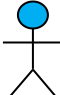
\includegraphics[scale=.3]{imagenes/actor.png}  }%iucluye la imagen del actor
\newcommand{\sistema}[0]{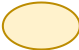
\includegraphics[scale=.3 ]{imagenes/system.png}  }%incluye la imagen del sistema
\newcommand{\finCU}[0]{\textit{- - - - Fin del caso de uso.}\\}
\newcommand{\finTA}[0]{\textit{- - - - Fin de la trayectoria.}\\}
\newcommand{\Tsubsection}[1]{\textcolor{myDarkBlue}{\subsection{#1}}}

%---------------------Titulo para los requisitos funcionales----------------%
\newcommand{\Dline}[2]{{\setlength{\parindent}{0pt}\textbf{\textcolor{myBlue}{\large{#1} \large{#2}}}} \\\rule[3mm]{110mm}{0.3mm}
\includegraphics[scale=.5]{imagenes/Documento.png}}%Linea de separadora 

%----------------------------Titulo para las reglas del negocio-------------------%
\newcommand{\DGline}[2]{\hypertarget{#1}{ }{\setlength{\parindent}{0pt}\textbf{\textcolor{myBlue}{\large{#1} \large{#2}}}} \\\rule[3mm]{110mm}{0.3mm}
\includegraphics[scale=.5]{imagenes/DocumentoG.png}}%Linea de separadora 
%----------------------------Titulo para los requisitos no funcionales-------------------%
\newcommand{\DVline}[2]{{\setlength{\parindent}{0pt}\textbf{\textcolor{myBlue}{\large{#1} \large{#2}}}} \\\rule[3mm]{110mm}{0.3mm}
\includegraphics[scale=.5]{imagenes/DocumentoV.png}}%Linea de separadora 

%----------------------------Titulo para los mensajes -------------------
\newcommand{\Mline}[2]{\hypertarget{#1}{ }{\setlength{\parindent}{0pt}\textbf{\textcolor{myBlue}{\large{#1} \large{#2}}}} \\\rule[3mm]{110mm}{0.3mm}
\includegraphics[scale=.5]{imagenes/Mensaje.png}}%Linea de 

%----------------link para hacer referencia a una regla de negocio---------------------%
\newcommand{\RNref}[2]{\hyperlink{#1}{#1 #2} }

%----------------Etiqueta para marcar en cual quier parte del documentop---------------------%
\newcommand{\Tlabel}[1]{\hypertarget{#1}{ }}

%----------------referencia para ir a las etiquetas previamente marcadas-------------------%
\newcommand{\Tref}[2]{\hyperlink{#1}{#2}}

%---------------------------Errores-----------------%
\newcommand{\TError}[2]{\hypertarget{TE#1:#2}{ }\textbf{#2:}}
\newcommand{\TEref}[2]{\hyperlink{TE#1:#2}{[Error #2]}}

%---------------------------Trayectoria alternativa-----------------%
\newcommand{\Talterna}[2]{\hypertarget{TA#1:#2}{ }\textbf{Trayectoria alternativa #2:}}
\newcommand{\TAref}[2]{\hyperlink{TA#1:#2}{[Trayectoria #2]}}
%-----------------------Titulo de los capítulos-----------------
\newcommand{\TChapter}[2]{\begin{tcolorbox}[adjusted title=flush center,halign title=flush center,titlerule=3mm,title=\ ] \chapter{#1} \centering \includegraphics[scale=1]{imagenes/alfabetoG/#2.png}  \end{tcolorbox}
\chaptermark{#1}% Nombre en el header
}



%---------------------Titulo para sección principal de Marco T----------------%
\newcommand{\MTtitle}[2]{\ \rule{135mm}{0.3mm}\ \\

{\setlength{\parindent}{0pt}\textbf{\textit{\textcolor{myDarkBlue}{\begin{huge}#1\end{huge} }}}}\ \\
\ \rule{135mm}{0.3mm}\\
\ \rule[3.5mm]{135mm}{0.1mm}\\ }%Linea de

%-----------------------------Caja de texto para ejemplos---------------------------------------%
\newtcolorbox[auto counter,number within=section,
crefname={bluebox}{blueboxes}]%
{mygraybox}[2][]{colbacktitle=white!30!black,colframe=white!30!black,fonttitle=\bfseries,
title=Cuadro \thetcbcounter: #2,#1}


%--------------Definimos un estilo con formato corto------------------------------------%

\newcommand{\HSection}[1]{
	
\fancypagestyle{plain#1}{
%\fancyhead[LE,RO]{\textsl{TRABAJOS I}}
\fancyhead[LE,RO]{\thesection.\textsl{ #1}}
%\renewcommand{\sectionmark}[1]{}
}
%\thispagestyle{plain#1}
\pagestyle{plain#1}

}

\newcommand{\HNSection}{

\fancypagestyle{plain}{
 \fancyhead[LE,RO]{\textsl{\rightmark}}
}
%\thispagestyle{plain#1}
\pagestyle{plain}

}



\renewcommand{\chaptermark}[1]{%
 \markboth{\MakeUppercase{%
 \chaptername\ \thechapter.%
 \ #1}}{}}

%----------------Incluimos la sección de bibliografía a la tabla de contenidos--------%

\let\OLDthebibliography=\thebibliography
\def\thebibliography#1{\OLDthebibliography{#1}%
\addcontentsline{toc}{chapter}{\bibname}}



\begin{document}

\renewcommand{\tablename}{Tabla} %Nombre de las tablas

    \begin{titlepage}

  \thispagestyle{empty}


  \begin{minipage}{.2\textwidth}
    \flushleft
%----------------------Logo IPN ---------------------------%
    \center{
\includegraphics[scale=.19]{imagenes/ipn.pdf}}


%----------------imagenLineasGuia---------------------------%    
    \vspace{20pt}

    \center{
      \rule{.5pt}{.6\textheight}
      \hspace{7pt}
      \rule{2pt}{.6\textheight}
      \hspace{7pt}
      \rule{.5pt}{.6\textheight}
    }
%----------------------Logo ESCOM ----------------------------%
    \center{
\includegraphics[scale=.07]{imagenes/logoescom.png}} 

  \end{minipage}
  \begin{minipage}{.8\textwidth}
  %---------------InfoTesis-------------------------%
    \flushright

    \center{

      \center{
        \LARGE{I}\large{NSTITUTO} \LARGE{P}\large{OLITÉCNICO} 
        \LARGE{N}\large{ACIONAL}
      } \\

      \rule{\textwidth}{1pt}\\
      \hrulefill\\[1cm]



      \LARGE{E}\large{SCUELA} \LARGE{S}\large{UPERIOR} \large{DE} \LARGE{C}\large{ÓMPUTO}\\[1cm]

      \large{ TRABAJO TERMINAL} \\[1cm]

      \textbf{ \LARGE{R}\LARGE{ecolector} \LARGE{y} \LARGE{clasificador} \LARGE{de}  
      \LARGE{noticias}}\\[1cm]
      \large{\textbf{2018-B013}}\\[1cm]


      \large{\textbf{PRESENTAN:}}\\[1cm]
      \large{CARLOS ANDRES HERNANDEZ GOMEZ}\\
      \large{LUIS DANIEL MEZA MARTÍNEZ}\\[1cm]


      \large{\textbf{DIRECTORES:  }}\\[.5cm]
      \large{\textbf{Dr.} JOEL OMAR JUÁREZ GAMBINO }\\
      \large{\textbf{Dra.} CONSUELO VARINIA GARCÍA MENDOZA }\\[0.5cm]

     \ \\
     Ciudad de México,\today

    }


  \end{minipage}
  \end{titlepage}

  
  
    \tableofcontents% indice de capítulos y secciones
    \listoffigures % indice de figuras
    \listoftables % indice de tablas

  \mainmatter %Iniciamos la número ración del indice

  %-------------------------------Capitulos----------%

    




\TChapter{Introducción}{alfa}




\ \\\\
\begin{Large}$\mathbf{E}$\end{Large}l artículo periodístico o noticia, es la información de un hecho de interés 
  ocurrido en un periodo de tiempo determinado. Constituye el elemento primordial en la información de la prensa y 
  del género básico del periodismo \citep{CU1}. Conocer los acontecimientos del mundo independientemente del tema, día o 
  lugar en el cual se han suscitado, tiene una gran importancia en la sociedad, se comparten por distintos medios de comunicación, 
  tales como la televisión, redes sociales, diarios, blogs y la radio. Nos permiten conocer la situación económica del país, logros 
  de la ciencia, desastres naturales, la situación en cuestión de inseguridad entre otros hechos. En el ámbito de las inversiones, 
  crean expectativas y eso a su vez puede modificar los planes de inversión en cualquier sector, siendo así de suma importancia 
  compartirlas de una forma eficaz \citep{CU2}.\\

El uso de páginas web como medio de comunicación está en incremento, permitiendo consultar noticias de distintos sitios como 
los periódicos electrónicos; su información al igual que un diario tradicional se encuentra dividida en secciones para facilitar 
la consulta, sin embargo, la clasificación suele variar en cada portal, incluso teniendo el mismo contenido. Un problema mayor se 
encuentra en los sitios independientes, los cuales no cuentan con una segmentación particular, haciendo difícil realizar una búsqueda eficaz.\\


\section{Problemática}


Los métodos tradicionales para la recopilación de información de los recolectores web (\textit{Crawler}), están basados en las etiquetas o 
marcadores que los sitos añaden a su código fuente, por ejemplo, algunos artículos periodísticos son etiquetados a la sección que pertenecen 
(política, deporte, cultura, etc). Sin embargo, existen muchas fuentes de información que no etiquetan sus publicaciones, incluso si la tarea 
es realizada, dicha segmentación no indica claramente el tipo de contenido; al consultar algunos de los portales mas visitados en México (en el giro del periodismo) 
se encuentra definida la sección deportes con varios sinónimos como \textbf{Universal deportes} (diario \text{El Universal}), \textbf{La afición} 
(\text{Milenio}), \textbf{Adrenalina} (\text{Excélsior}), etc. Como este ejemplo se encuentran más. Las noticias son segmentadas de forma tan diversa que 
ha complicado su búsqueda en la Internet.\\


Para definir las etiquetas o marcadores con los cuales se clasifica la información de los sitios web, se requiere un proceso manual de análisis de 
la información. Este proceso implica tiempo y esfuerzo por parte de las personas que realizan el trabajo. Por lo anterior se plantea la necesidad de crear 
métodos para automatizar esta tarea. 

\section{Justificación}


Hoy en día existen distintas maneras de informarse acerca de los acontecimientos más recientes, por ejemplo, la televisión, blogs, redes sociales, foros,
diarios, etc. Esto ha provocado que la información se encuentre dispersa y
se deba acceder a múltiples recursos para ser recopilada, implicando
una inversión de tiempo y esfuerzo. Para facilitar esta tarea, existen herramientas
que hacen la búsqueda de noticias de interés para el usuario en forma automática. Sin embargo, dichas herramientas requieren que los sitios a consultar 
tengan etiquetas definidas y homogéneas.\\

Según el díario El Economista \citep{CU3} el sitio web Animal Político\footnote{www.animalpolitico.com}
ocupa el lugar número cuatro en el ranking de medios nativos digitales, clasifica sus noticias de una manera poco habitual para los lectores como la sección
\textbf{El sabueso}, \textbf{El plumaje}, \textbf{Hablemos de . . . }, entre otras, lo que hace complicado obtener los artículos con los métodos tradicionales 
de recopilación que, se basan sólo en las etiquetas que identifican cada sección y no el contenido de las noticias.

%\lhead{ (www.animalpolitico.com)}
%\thispagestyle{ESTILO}

\section{Solución propuesta}

Se propone crear una aplicación web que recolecte y clasifique noticias de acuerdo a su contenido y periodo de publicación. Finalmente, las noticias
que satisfagan ambos filtros (Tipo de contenido y fecha de publicación) serán mostradas al usuario.

%---------------------------------------------------------------------------------------

\Tlabel{cp1:objetivoG}
\section{Objetivo general}

  Crear un recolector de noticias, el cual permita recopilar información de diferentes fuentes como diarios, sitios de noticias, foros y mediante el 
  análisis automático de su contenido muestre aquellas noticias que satisfagan los filtros establecidos por el usuario.
  

\section{Objetivos específicos}
\begin{itemize}
  \item Desarrollar un recolector de noticias, el cual permita obtener información de diferentes fuentes como diarios, sitios de noticias, blogs y foros
  \item Analizar de forma automática el contenido de las noticias para satisfacer los filtros establecidos por el usuario
  \item Mostrar las noticias que cumplieron con los filtros establecidos, así como su enlace (URL) para redirigirlos a la página de la noticia
  \item Afinar el clasificador de noticias realizado en el trabajo terminal 2017-A042 para utilizarlo en el contexto de esta propuesta (filtro de sección) 
\end{itemize}
  \newpage
  \Tlabel{cp2:estadodelarte}
\TChapter{Estado del arte}{beta}
\ \\\\
%-----------------------------------Introducción---------------------------------------------%
\section{Introducción}


El uso de la información digital ha superado la producción de libros y publicaciones impresas, este fenómeno ha influenciado la producción de bibliotecas digitales, publicaciones electrónicas; Se ha incrementado el uso de las redes sociales, correos electrónicos, creando un gran repositorio de información útil, el cual puede ser analizado\citep{CD1}.\\

Debido a la necesidad de procesar grandes volúmenes de datos recolectados de Internet, se han desarrollado diversas investigaciones entorno a esta tarea. A continuación se muestran distintos artículos nacionales e internacionales relacionados al campo de investigación (clasificación de noticias), de igual forma se muestran herramientas web que desempeñan un trabajo similar al propuesto (sitio web de noticias). Cabe destacar que el área de interés cuenta con un amplio desarrollo, no obstante solo se mencionan los trabajos más relevantes para este documento.

%-------------------------------Trabajos nacionales-----------------------------------------%

\section{Trabajos nacionales}


%----------------------------------TN1-------------------------------%
\begin{large}
	 \subsection[Clasificación de noticias de diarios]{Clasificación de noticias de diarios de circulación nacional mediante aprendizaje automático }
\end{large}


En este trabajo terminal de la Escuela Superior de Cómputo \citep{CD2} los autores clasifican mediante técnicas de aprendizaje automático, noticias de diarios de circulación nacional en las diferentes secciones en que en estos se dividen. Se recolectaron 4,027 artículos de tres diarios de circulación nacional: \textbf{El universal}, \textbf{La jornada} y \textbf{Excélsior}. 3,624 noticias fueron utilizadas para la etapa de entrenamiento y 407 para hacer las pruebas.\\

El trabajo utiliza  pre-procesamiento de información con la técnica tokenización y lematización (ver \Tref{CP1}{Capítulo 3}). El mejor resultado en las pruebas se dio en la combinación del algoritmo \textbf{TF-IDF} para extraer las características y \textbf{Máquinas de soporte vectorial} para la clasificación de artículos, se obtuvo un 79.81\% de exactitud, \textit{i.e} 8 de cada 10 noticias son clasificadas correctamente.\\


%----------------------------------TN2-------------------------------%

\begin{large}
	 \subsection[Desastres naturales en México]{Clasificación automática de textos de desastres naturales en México}
\end{large}

En este trabajo se propone clasificar noticias en el ámbito \textbf{desastres naturales} \citep{CD9}, utilizando estrategias de reducción de dimensionalidad conocidas como, umbral en la frecuencia y ganancia en la información, los métodos de clasificación utilizados fueron el clasificador simple de Bayes y vecinos más cercanos.\\

Se utilizaron 375 noticias del periódico Reforma como conjunto de entrenamiento, se clasificaron en artículos relevantes e irrelevantes, de los cuales 11.5\% de noticias eran relevantes y el 88.5\% restante eran irrelevantes. Una vez obtenido el conjunto de noticias se procedió con un pre-procesamiento, el cual reduce el tamaño de los documentos, eliminando la parte de los textos que no brindan información útil, posteriormente se realizó un indexado: Los documentos son representados por vectores de palabras en un espacio de dimensión n, para realizar una reducción de dimencionalidad. Finalmente se utilizaron técnicas de clasificación (Algoritmo simple de Bayes) con el cual se obtuvo un resultado de 97\% de efectividad en la clasificación de noticias.\\


%----------------------------------TN3-------------------------------%

\begin{large}
	 \subsection[Extraer información de noticias de DN]{Usando aprendizaje automático para extraer información de noticias de desastres naturales}
\end{large}


Este trabajo describe un sistema basado en métodos de Aprendizaje automático que mejora la adquisición de datos de desastres naturales\citep{CD11}. Este sistema automáticamente llena una base de datos de desastres naturales con la información extraída de noticias de periódicos en línea. En particular, se extrae información acerca de cinco tipos de desastres naturales: huracanes, temblores, incendios forestales, inundaciones y sequías. Los algoritmos implementados para la extracción de información son los siguientes: 

\begin{itemize}
	\item Naive bayes
	\item Maquinas de soporte vectorial
	\item C4.5
\end{itemize} 

Los resultados experimentales en una colección de noticias en Español muestran la eficacia del sistema propuesto tanto para detectar documentos relevantes sobre desastres naturales (alcanzando una medida-F de 98\%), así como para extraer hechos relevantes para ser insertados en una base de datos dada (alcanzando una medida-F de 76\%).

%------------------------------Trabajos internacionales--------------------------------------%

\section[Trabajos I]{Trabajos internacionales}

%----------------------------------TI1-------------------------------%
\begin{large}
	 \subsection{Clasificador de noticias usando autoencoders}
\end{large}

En este trabajo se propone la clasificación de noticias utilizando \textit{Deep Learning} \citep{CD3}, las noticias se clasificaron en las siguientes categorías:

\begin{itemize}
	\item Deportes
	\item Política
	\item Espectáculos
	\item Economía
	\item Policía
\end{itemize}
El alcance que tiene es:
\begin{itemize}
	\item Local (Valparaíso)
	\item Nacional (Chile)
	\item Internacional (resto del mundo)
\end{itemize}

El clasificador se construyó utilizando una base de datos con 542 noticias etiquetadas con los criterios anteriores, las características se obtuvieron utilizando Autoencoders (AE) para entrenar una Red Neuronal Artificial (ANN).
Los resultados obtenidos con 156 noticias fue una tasa de éxito del 92.3\% para la clasificación de la categoría y un 87.2\% para el clasificador de alcance.
La tasa general de éxito, categoría y alcance fue de 83.75\%.\\

%----------------------------------TI2-------------------------------%
\begin{large}
	 \subsection{Document classification for newspaper articles}
\end{large}

El trabajo clasifica artículos de la universidad \textit{Massachusetts Institute of Technology} \citep{CD4} en las categorías: \textit{Arts}, \textit{Features}, \textit{News}, \textit{Opinion}, \textit{Sports}, \textit{World}. Para la etapa de entrenamiento se ocupó un total de 480 artículos por sección, y para realizar las pruebas 120 noticias. El mejor resultado se obtiene utilizando \textit{Multi-Variate Bernoulli Featureset} como algoritmo de extracción de características y \textit{Naive Bayes Classification} como algoritmo clasificador ya que, obtiene  un 77\% de exactitud.\\

%----------------------------------TI3-------------------------------%

%----------------------------------TI4-------------------------------%

\begin{large}
	 \subsection[Category classification and topic discovery]{Category classification and topic discovery of japanese and english news articles}
\end{large}


Este trabajo desarrolla un algoritmo de aprendizaje supervisado (ver \Tref{CP1}{Capítulo 3}) para la clasificación de noticias en categorías (como política, deportes, tecnología) y temas (sección de deportes: tenis, fútbol, golf) en diferentes lenguajes, además se especializa en descubrir y clasificar temas emergentes en Internet \citep{CD6}. Se ocupa un método pare extraer palabras claves en cualquier idioma propuesto por Bracewell \citep{CD5}, el cual obtiene palabras de muy alta calidad de un solo documento. Se definieron 8 secciones posibles a las que puede ser clasificado el artículo proporcionado, los cuales son:

\begin{itemize}

	\item \textit{Business} 
	\item \textit{Politics} 
	\item \textit{Crime and Misfortune} 
	\item \textit{Health} 
	\item \textit{Sports} 
	\item \textit{Entertainment} 
	\item \textit{Technology} y 
	\item \textit{Science and Nature}

\end{itemize}



Con ejemplos positivos el método entrena un clasificador para cada categoría.
El proceso de clasificación consta de 4 pasos:

\begin{enumerate}
	\item Las palabras claves son extraídas del documento dado.
	\item la probabilidad de pertenencia a cada categoría es calculado.
	\item Se crea un umbral de pertenecía dinámico.
	\item Finalmente se asigna el artículo a una categoría.
\end{enumerate}

Para desarrollo del método se implementó en lengua ingles y japones, se ocuparon 1,000 artículos descargados de sitios como Yahoo, de cada idioma. 800 se ocuparon en el entrenamiento y 200 para realizar pruebas. \\

Para contar con un punto de comparación se clasifico con algoritmos  ya probados: \text{Naive bayes}, \text{Árboles de decisión}, \text{Máxima entropia} y el propuesto por el artículo. El mejor resultado fue dado por  el método propuesto obteniendo 63.4\% en exhaustividad, 68.6\% en precisión y 65.9\% en la media-F.\\ 


%----------------------------------TI5-------------------------------%

\begin{large}
	 \subsection[Automatic news articles classification in indonesian]{Automatic news articles classification in indonesian language by using naive bayes classifier method}
\end{large}

El artículo clasifica noticias ocupando el algoritmo clásico \textit{Naive Bayes} \citep{CD7}. El método propuesto consiste en 3 tareas importantes: Pre-procesamiento el cual consiste en la siguiente serie de pasos: 
 
\begin{enumerate}

	\item \textit{Case folding}: Proceso para convertir todas letras en minúsculas.
	\item \textit{Parsing}: Es el proceso de convertir oraciones en palabras.
	\item \textit{Stopwords elimination}: Es el proceso de eliminar palabras que se repiten con mucha frecuencia y no es información útil (Una definición mas amplia se da en el capítulo 3).
	\item \textit{Stemming}: Es un proceso de corte o eliminación de afijos en una palabra. Las variantes de los afijos son prefijos, sufijos, in-fijos y con-fijos (la combinación de prefijos y sufijos).

\end{enumerate}	

La segunda tarea es la etapa de entrenamiento del algoritmo y por último la clasificación de artículos. Cabe destacar que el método \textbf{Frecuencia de término} (Frecuencia de aparición de una palabra en un documento dado) es utilizado en la etapa de aprendizaje. Las secciones definidas en el trabajo son: 

\begin{itemize}

	\item \textit{Economy}
	\item \textit{Sport}
	\item \textit{Tecnology}
	\item \textit{Healt} 
	\item \textit{Metropolitan}

\end{itemize}

Para el proceso de aprendizaje se ocuparon 50 noticias por tópico, las cuales fueron recolectadas de los sitios web \textit{Kompas}\footnote{Sitio web Indu de noticias: https://www.kompas.com}, \textit{Republika}\footnote{Sitio ya no disponible: http://www.republika.com} y \textit{Suara pembaruan}\footnote{Sitio web Indu: https://sp.beritasatu.com}.Las pruebas fueron realizadas con 12 noticias por sección. Además para tener una métrica en la eficiencia del método se calculó la precisión, exhaustividad y la media-F. Los resultados muestran que el método de \text{Naive bayes} es un clasificador con una media-F de 92.26\%.\\ 

%----------------------------------TI6-------------------------------%

\begin{large}
	 \subsection{News article text classification in indonesian language}
\end{large}

Este documento busca el mejor algoritmo de clasificación en lenguaje Indu, comparando la eficiencia de algoritmos de selección de características (Palabras clave) y de clasificación de noticias \citep{CD8}. Las secciones definidas por el artículo son las siguientes, \textit{Economy}, \textit{Health}, \textit{Sports}, \textit{Politic} y \textit{Tecnology}; El trabajo realiza pre-procesamiento de datos con  los métodos \textit{lemmatization} y \textit{Stopwords} para reducir el ruido en la información. Para la obtención de noticias se hace uso de la técnica \textit{crawling}(ver \Tref{CP1}{Capítulo 3}) en el sito \textit{ccnnindonesia}\footnote{Sitio web de noticias: wwww.ccnnindonesia.com}. Se obtuvieron 1,000 artículos para cada sección. 800 se usaron para la etapa de entrenamiento y 200 para realizar pruebas. Se muestra la lista de los algoritmos implementados:

\begin{itemize}
	\item Selección de características:
	\begin{itemize}
		\item \textit{Singular Value Decomposition}
		\item \textit{Term frequency-inverse document frequency}
	\end{itemize}

	\item Clasificación:
	\begin{itemize}
		\item \textit{Support vector machine}
		\item \textit{Naive bayes classifier}
		\item \textit{Gaussean naive bayes}
		\item \textit{Multinominal naive bayes}
		\item \textit{Multivariate naive bayes}
		\item \textit{Bernulli naive bayes}
	\end{itemize}
\end{itemize}

 El mejor resultado es en combinación de \textit{Term frequency-inverse document frequency} y  \textit{Multinominal naive bayes} con la precisión y exhaustividad mas alta el cual está alrededor de 98.4\% con un tiempo de 0.702 segundos, seguido de \textit{Term frequency-inverse document frequency} y \textit{Bernulli naive bayes}(BNB)  con 98.2\% en precisión y exhaustividad con un tiempo de .701 segundos.


%------------------------------Herramientas Disponibles-------------------------------------%

\section[Herramientas D]{Herramientas disponibles}


Entre las herramientas de trabajo que son de utilidad para el procesamiento de lenguaje natural y aprendizaje automático se encuentran:\\

%------------------------------loud Natural Language-------------------------------------%

\begin{large}
	 \subsection{Cloud natural language}
\end{large} 

\textit{Google Cloud Natural Language} \citep{CD12}   revela la estructura y el significado del texto con modelos potentes de aprendizaje automático previamente entrenados en una API de REST fácil de usar y con modelos personalizados se puede utilizar para extraer información sobre personas, lugares, eventos y muchos otros datos, que se mencionan en documentos de texto, artículos periodísticos o entradas de blog. También se puede utilizar para comprender las opiniones sobre los productos expresadas en los medios sociales o analizar la intención en las conversaciones de los clientes que se den en un centro de atención telefónica o una aplicación de mensajería.\\

%----------------------------------------Googlebot-------------------------------------%

\begin{large}
	 \subsection{Googlebot}
\end{large}

Es el crawler diseñado por Google para indexar el contenido nuevo o actualizado de Internet.
Googlebot \citep{CD13} no sólo tiene la capacidad de rastrear e indexar los sitios web de Internet, sino que además puede extraer información de ficheros como pueden ser PDF, XLS, DOC, etc.
Una vez el contenido está indexado, el servidor lo clasifica y establece un orden de relevancia para las distintas búsquedas que pueda efectuar un usuario, es decir, lo posiciona.\\


%----------------------Watson natural language classifier----------------------------------%

\begin{large}
	 \subsection{Watson natural language classifier}
\end{large}

Watson NLC \citep{CD14} aplica técnicas de computación cognitiva para analizar un texto y proporcionar la clase que mejor encaja entre un conjunto de clases predefinidas a partir de un texto corto.
Al ser un clasificador, esta compuesto de ciertos pasos, en primera instancia se necesitan de clases las cuales son etiquetas que identificarán el texto analizado y será la salida proporcionada por el clasificador; posteriormente se debe tomar en cuenta que se necesita de una colección de textos, los cuales proporcionarán apoyo para que el clasificador logre identificar las clases ingresadas posteriormente teniendo todos estos datos se logra entrenar al clasificador, el cual proporcionará una salida dependiendo a los datos que fueron utilizados.



  \newpage
  
\Tlabel{CP1}\TChapter{Marco teórico}{gama}
\ \\
%---------------------------------Introducción--------------------------------%
En este capítulo se expondrán de manera detallada y ordenada el conjunto de conocimientos que permitirán comprender y analizar el tema propuesto. \\

La Figura \ref{fig:MarcoT} muestra los campos abarcados por la investigación.
A continuación cada área sera desarrollada con los conceptos de interés para la solución propuesta.\\

\begin{figure}[H]
	\centering
	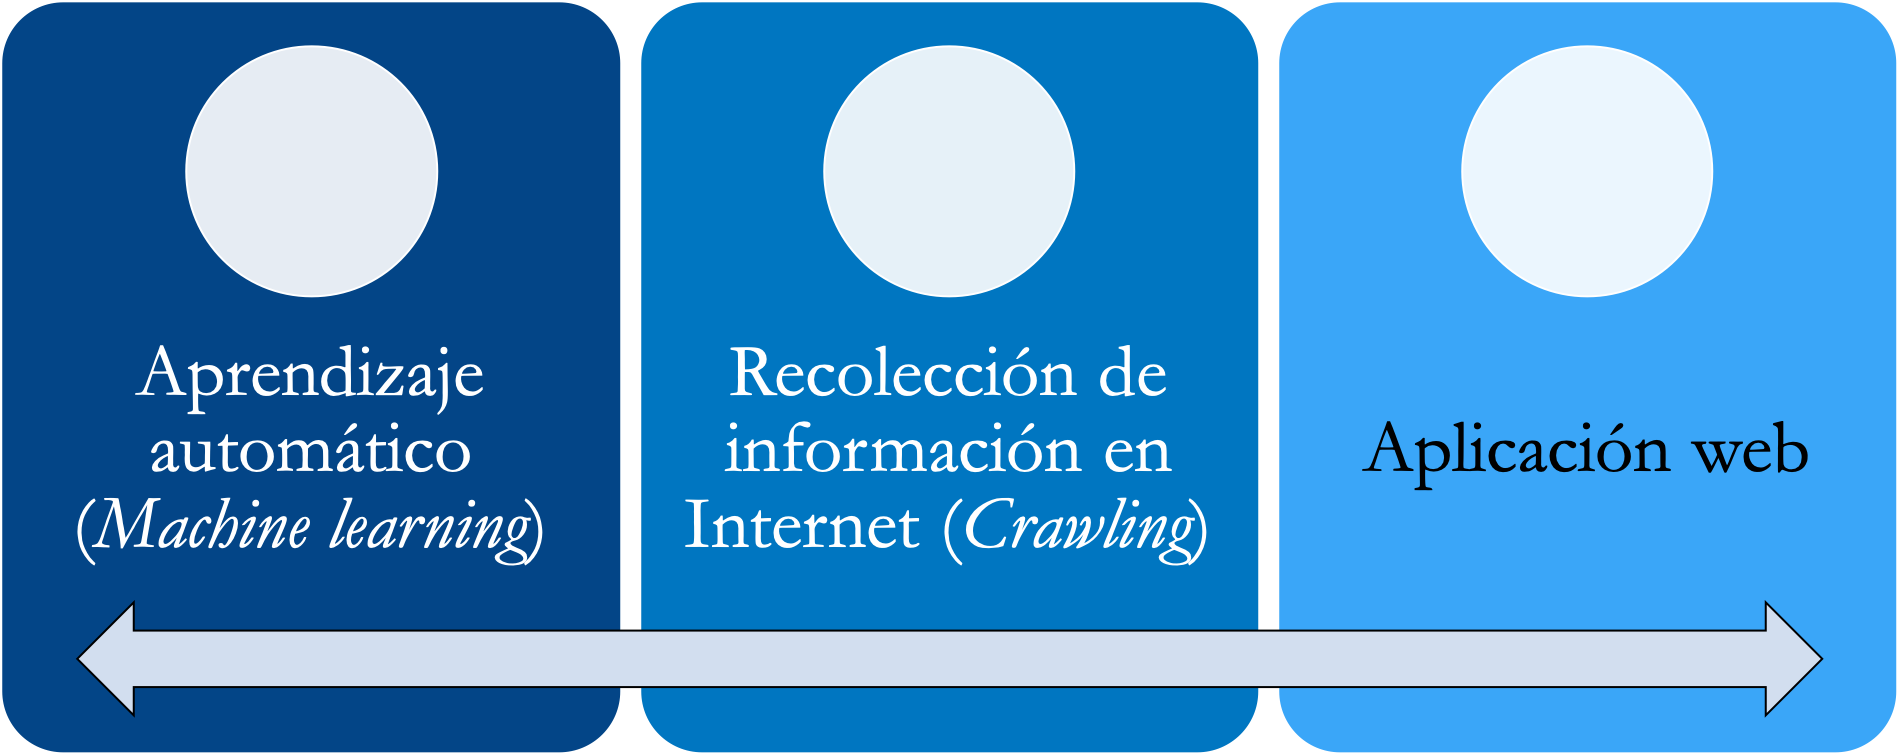
\includegraphics[scale=.45]{imagenes/Capitulo3/Marco.png}
	\caption{Campo de estudio}
	\label{fig:MarcoT}
\end{figure}
%---------------------------------Conceptos-------------------------------------%
\ 

%----------------------------------------Aprendizaje automático-------------------------------%
%---------------------------------------------------------------------------------------------%

\MTtitle{Aprendizaje automático}


%------------------------------------Inteligencia Artificial-------------------------------%
\section{Inteligencia Artificial}

Son muchas las definiciones que se encuentran de la inteligencia artificial o IA, en sus inicios se propone como las  actividades asociadas al pensamiento humano, tareas como, toma de decisiones, resolución de problemas y aprendizaje \citep{CT19}. Con el paso de los años se ha acuñado una definición mas completa: ``la Inteligencia Artificial es una ciencia orientada al diseño y construcción de máquinas que implementen tareas propias de humanos dotados de inteligencia'' \citep{CT1}.\\


Esta ciencia contribuye en el desarrollo de diversos campos de investigación como, Redes neuronales, Computación evolutiva, Algoritmos genéticos, Programación Genética, Teoría del caos. Además tiene un campo amplio de aplicaciones en la sociedad \citep{CT20}, a continuación se muestran algunos ejemplos:

\begin{itemize}

	\item \textbf{Vehículos robóticos}: Un auto robótico sin conductor llamado STANLEY aceleró a través del terreno de Mojave a 22 mph (\textit{miles per hour}, por sus siglas en ingles), terminando el curso de 132 millas primero para ganar el Gran Desafío DARPA 2005

	\item \textbf{Reconocimiento de voz}: Un viajero que llama a \textit{United Airlines} para reservar un vuelo puede tener la conversación completa guiada por un sistema automático de reconocimiento de voz y gestión de diálogos

	\item \textbf{Planificación y programación autónoma}: A cien millones de millas de la Tierra, el programa \textit{Remote Agent} de la NASA se convirtió en el primer programa autónomo de planificación a bordo para controlar la programación de operaciones de una nave espacial

	\item \textbf{Robótica}: \textit{iRobot Corporation} ha vendido más de dos millones de aspiradoras robóticas \textit{Roomba} para uso doméstico

	\item \textbf{Máquina traductora}: Un programa de computadora  traduce automáticamente del árabe al inglés

\end{itemize} 
 

%----------------------Procesamiento de lenguaje natural-------------------------------------%

\section{Procesamiento de lenguaje natural}
\HSection{PROCESAMIENTO DE LN}

El procesamiento de lenguaje natural es una disciplina de la Inteligencia Artificial que se ocupa de la formulación e 
investigación de mecanismos computacionales para la comunicación entre personas y maquinas mediante el uso de Lenguajes 
Naturales.\\

Este campo incluye diferentes técnicas para interpretar el lenguaje humano, que van desde los métodos 
estadísticos y del aprendizaje basado en máquina hasta los enfoques basados en reglas y algorítmicos. Se necesita una amplia variedad 
de métodos porque los datos basados en texto y en voz varían ampliamente, al igual que las aplicaciones prácticas.\\

Dentro de la amplia gama de técnicas para el procesamiento de lenguaje natural, en este trabajo se harán uso de dos de estas técnicas llamadas \textbf{Tokenización} y \textbf{Lematización}. A continuación se describen cada una de ellas junto con un proceso previo llamado pre-procesamiento.\\


%------------------------------------Pre-procesamiento------------------------%

\subsection[Pre-procesamiento]{Pre-procesamiento}


Cuando se recupera  información de la web, se debe limpiar el texto ya que contiene etiquetas definidas por el hipertexto (ver \Tref{cp3:html}{HTML}). Se deben buscar los bloques que brinden información útil para el ámbito de estudio, algunas secciones contienen publicidad o información no relacionada a los datos de interés. Para esto se tiene que realizar un análisis para discriminar la información útil \citep{CD1}. A continuación se muestra un ejemplo de un texto que que requiere ser pre-procesado\\

\begin{mygraybox}[label={box:cp3:texto}]{Texto de ejemplo} 
$<h1>$¡Estudiantes politécnicos apoyan académicamente a alumnos de primaria!$</h1>$\\

$\infty$
$<p>$El Secretario de Educación Pública \Tribar[1][blue][blue!50][blue!20], Esteban Moctezuma Barragán, ha subrayado la importancia \#\#\# de que en la Nueva Escuela Mexicana el Instituto Politécnico Nacional (IPN)\dSmiley, contribuya a fortalecer la educación básica.$</p>$\\
$<!--\ -->$
\end{mygraybox}
\ \\
Como se puede apreciar en el Cuadro \ref{box:cp3:texto} algunas etiquetas requieren ser descartadas para poder obtener únicamente el contenido de la noticias, por ejemplo se debe eliminar el \textit{hipertexto} ( $<h1>$,$</p>$ ) los emojis ( \dSmiley,\Tribar[1][blue][blue!50][blue!20] ) y los símbolos ( $\infty$,\# ). El cuadro \ref{box:cp3:textolimpio} muestra el resultado de limpiar el contenido.\\

\begin{mygraybox}[label={box:cp3:textolimpio}]{Texto limpio} 
¡Estudiantes politécnicos apoyan académicamente a alumnos de primaria!\\

El Secretario de Educación Pública, Esteban Moctezuma Barragán, ha subrayado la importancia  de que en la Nueva Escuela Mexicana el Instituto Politécnico Nacional (IPN), contribuya a fortalecer la educación básica.
\end{mygraybox}
	%\item \textbf{Remover stop-words}: Son pronombres y preposiciones que deben ser removidas para mejorar la compresión del texto.

	%\item  \textbf{Stemming, case-folding, punctuation}: Las palabras que derivan de la misma raíz como hundimiento, se hundió, se reducen a hundir. Una palabra puede tener diferentes significados dependiendo el contexto como la palabra \'Rosa\' puede hacer referencia a una flor o el nombre de una persona, por lo tanto se requiero la heurística del lenguaje específico para poder tomar una decisión en como debe ser interpretada. Los signos de puntuación como el guión medio deben ser tratados con mucho cuidado para realizar una buena tokenización.

%-----------------------------------------Tokenización-------------------------------------%

\subsubsection{Tokenización}

Es el proceso que descompone los textos de una colección en sus unidades mínimas, las palabras
o términos propiamente dichos. A tales elementos se les denomina tokens que conforman una lista de
items que se utilizan para su análisis estadístico, ling{\"u}ístico, de almacenamiento y posteriormente de
recuperación de información. Los tokens a su vez pueden ser identificados mediante una codificación
ASCII o en su defecto UNICODE. De hecho, este proceso permite la identificación de cadenas de caracteres de
forma unívoca, de cara a posteriores tratamientos de depuración, eliminación de signos de puntuación
o la reducción morfológica \citep{CT12}.\\

Continuando con el ejemplo del Cuadro \ref{box:cp3:textolimpio}, se procede a realizar la tokenización del contenido. El Cuadro \ref{box:cp3:tokenizado} muestra el texto dividido en tokens.\\

\begin{mygraybox}[label={box:cp3:tokenizado}]{Texto tokenizado} 
\begin{large}\textbf{¡}\end{large} Estudiantes politécnicos apoyan académicamente a alumnos de primaria \begin{large}\textbf{!}\end{large}\\

El Secretario de Educación Pública \begin{Large}\textbf{,}\end{Large} Esteban Moctezuma Barragán \begin{Large}\textbf{,}\end{Large} ha subrayado la importancia  de que en la Nueva Escuela Mexicana el Instituto Politécnico Nacional \begin{Large}\textbf{(}\end{Large} IPN \begin{Large}\textbf{)}\end{Large} \begin{Large}\textbf{,}\end{Large} contribuya a fortalecer la educación básica \begin{Large}\textbf{.}\end{Large}
\end{mygraybox}
\ \\
Como se puede observar se ha separado por un espacio las palabras, donde cada una representa un token. Ademas los signos de admiración (\begin{large}\textbf{! ¡}\end{large}), los signos de puntuación (\begin{large}\textbf{. ,}\end{large}) y los paréntesis (\begin{large}\textbf{( )}\end{large}), se han divido como tokens independientes.

%-----------------------------------------Lematización-------------------------------------%

\Tlabel{cp3:lematizacion}
\subsubsection{Lematización}

Es el proceso lingüstico que, dada una palabra flexionada se encuentra su
lema. Una palabra flexionada es cuando está en plural, en femenino conjugada,
diminutivo o en superlativo. El lema es la palabra que está en singular para
sustantivo, singular masculino para adjetivo e infinitivo para un verbo \citep{CT13}. Ejemplo:

	\begin{itemize}
		\item amigos, amiga, amiguitos-> Amigo
		\item soy, son, es->Ser
	\end{itemize}

Cabe mencionar que existen diversos grados de lematización:

	\begin{itemize}
		\item Mórfólogica: Es la anteriormente explicada
		\item Sintáctica: Toma en cuenta el contexto donde se encuentra la palabra

	\end{itemize}

En este trabajo se utilizado el grado morfológico. Continuando con el ejemplo tokenizado ( Cuadro \ref{box:cp3:tokenizado} ), El Cuadro \ref{box:cp3:lematizado} muestra el contenido del texto lematizado.\\

\begin{mygraybox}[label={box:cp3:lematizado}]{Texto Lematizado} 
\begin{large}\textbf{¡}\end{large} estudiante politécnicos apoyar academia a alumno de primaria \begin{large}\textbf{!}\end{large}\\

el secretario de educar pública \begin{Large}\textbf{,}\end{Large} esteban moctezuma barragán \begin{Large}\textbf{,}\end{Large} haber subrayar el importar  de que en el nuevo escuela mexicano el instituto politécnico nacional \begin{Large}\textbf{(}\end{Large} ipn \begin{Large}\textbf{)}\end{Large} \begin{Large}\textbf{,}\end{Large} contribuir a fortaleza el educar básico \begin{Large}\textbf{.}\end{Large}
\end{mygraybox}
\ \\



%------------------------------------Apredizje automático-------------------------------%
\section{Aprendizaje Automático}

El Aprendizaje Automático es una rama de la Inteligencia Artificial; permite desarrollar algoritmos que tienen la capacidad de extrapolar (\textit{i.e} predecir) los cambios que se acontecen en una tarea específica \citep{CT2}.\\

El campo utiliza una variedad de algoritmos que aprenden iterativamente de un conjunto de
datos para describir y predecir resultados. A medida en la cual los algoritmos de 
entrenamiento obtienen datos es posible obtener modelos más precisos. Existen cuatro clasificaciones en los métodos \citep{CT21}:

\begin{itemize}

	\item \textbf{Aprendizaje supervisado}: Se proporciona un conjunto de datos de entrenamiento con las respuestas correctas y, con base a este conjunto de 
	entrenamiento, el algoritmo genera un modelo para responder correctamente a todas 
	las entradas posibles

	\item \textbf{Aprendizaje no supervisado}: No se proporcionan datos de entrenamiento, el algoritmo intenta identificar similitudes entre las entradas para clasificar en conjuntos. El enfoque estadístico del aprendizaje no 
	supervisado se conoce como estimación de densidad

	\item \textbf{Aprendizaje reforzado}: Está en algún lugar entre el aprendizaje supervisado y no supervisado. Se indica al algoritmo cuando la respuesta es incorrecta, sin embargo no se informa
	cómo corregirlo. Tiene que explorar y probar diferentes posibilidades hasta que resuelva 
	cómo obtener la respuesta correcta

	\item \textbf{Aprendizaje evolutivo}: La evolución biológica puede verse como un proceso de aprendizaje: los organismos biológicos se adaptan para mejorar sus tasas de supervivencia 
	y la posibilidad de tener descendientes en su entorno. Este comportamiento es modelado, 
	usando un modelo física, el cual corresponde a una puntuación en la 
	solución actual

\end{itemize}

Cabe mencionar que el método implementado en este trabajo es el aprendizaje supervisado, en la sección 3.5 (ver \Tref{cp3:asupervisado}{Aprendizaje supervisado} ) se detalla este enfoque.\\

El aprendizaje automático se puede aplicar a una amplia gama de problemas comerciales, desde la detección de fraudes hasta la orientación al cliente y la recomendación de productos, al monitoreo industrial en tiempo real, el análisis de sentimientos y el diagnóstico médico. Puede asumir problemas que no pueden administrarse manualmente debido a la gran cantidad de datos que deben procesarse \citep{CT22}. Cuando se aplica a grandes conjuntos de datos, a veces puede encontrar relaciones tan sutiles que ninguna cantidad de escrutinio manual las descubriría nunca. Y cuando muchas de estas relaciones ``débiles'' se combinan, se convierten en predictores fuertes.





%------------------------------------Apredizje automático para texto------------------------%

\section{Aprendizaje automático para texto}
\HSection{AA PARA TEXTO}

La extracción de información útil con varios tipos de algoritmos estadísticos es denominado \textbf{Extracción de datos} (\textit{text mining}), \textbf{Analítica de texto} (\textit{text analytics}) o \textbf{Aprendizaje automático para texto} (\textit{Machine learning for text}) \citep{CD1}. En los últimos años este campo ha incrementado por el desarrollo de la web, redes sociales, correos electrónicos, bibliotecas virtuales. Algunas de las aplicaciones son las siguientes:

\begin{itemize}

	\item Etiquetar la web, permite al usuario encontrar paginas de interés

	\item Los proveedores de correos, utilizan la información almacenada para mostrar publicidad de interés al usuario

	\item Algunas páginas ordenan su contenido de acuerdo a su importancia

	\item El análisis de las opiniones es un campo de importancia así como el análisis de sentimientos		

\end{itemize}

El orden de las palabras en un texto brindan un significado semántico el cual no puede ser inferido  solo con la frecuencia de las palabras. Sin embargo, se pueden hacer varias predicciones sin contemplar la semántica. Existen dos tipos de representaciones que son populares:

\begin{itemize}
	\Tlabel{cp3:bolsap}
	\item \textbf{Texto como una bolsa de palabras}: Es la representación mas común. No se contempla el orden de las palabras en el proceso. El conjunto de palabras en el documento se convierten en una representación multidimencional dispersa, el cual corresponde a la dimensión en esta representación. Se utiliza para la clasificación, sistemas de recomendación

	\item \textbf{Texto como un conjunto de secuencias}: En esta representación se extraen sentencias, el orden de las palabras si importa. La unidad son sentencia o párrafos. Es utilizado en aplicaciones que necesitan un fuerte uso de la semántica, esta área se acerca mucho al modelado de lenguaje
\end{itemize}


%----------------------------------Representación del texto--------------------------%
\Tlabel{cp3:representaciont}
\subsection{Representación del texto}

Los métodos de Aprendizaje Automático requieren que la información de la cual aprenderán esté representada en un
formato que facilite su procesamiento. Generalmente esta representación es mediante vectores de valores numéricos. 
Cuando se requiere utilizar estos métodos con información en forma de texto, dicha
información debe ser transformada para generar una representación más adecuada, los métodos mas comunes son: frecuencia, binaria y TF-IDF.\\ 


En este trabajo se utilizarán las dos primeras representaciones basandose en los resultados que han obtenido en el estado del arte. Por lo que sólo se describirán estas dos técnicas junto un ejemplo de su uso.\\


La extracción de características cuenta con dos tareas importantes: formar el vocabulario y crear un vector de características. Para ejemplificar esta tarea observe el Cuadro \ref{box:cp3:corpus} el cual es un corpus de 4 oraciones. Una vez realizado el proceso de extracción de características se obtiene el vocabulario el cual el mostrado en el Cuadro \ref{box:cp3:caracteristicas}.\\\\

\begin{mygraybox}[label={box:cp3:corpus}]{Corpus} 
\begin{equation*}
\begin{bmatrix}
Este&es&el&primer&texto&!!\\
Este&texto&es&el&segundo&texto&???\\
Y&este&es&el&tercero\\
Es&este&el&primer&texto&????\\
\end{bmatrix}
\end{equation*}
\end{mygraybox}
\ \\
\begin{mygraybox}[label={box:cp3:caracteristicas}]{Vocabulario} 
\begin{equation*}
\begin{bmatrix}
es  & este & el & texto & primer & segundo & tercero & y & ? & !
\end{bmatrix}
\end{equation*}
\end{mygraybox}

Las características son extraídas de 2 formas, binario(donde 1 representa la presencia de la característica y 0 la ausencia) y por frecuencia (donde se cuenta el número de veces que cada característica aparece). Continuando con el ejemplo del Cuadro \ref{box:cp3:corpus} se extraen las características por frecuencia y el resultado se muestra en el Cuadro \ref{box:cp3:frecuencia}, mientras que el Cuadro \ref{box:cp3:binario} muestra las características extraídas de forma binaria.\\


\begin{mygraybox}[label={box:cp3:frecuencia}]{Representación por frecuencia} 
\begin{equation*}
\begin{bmatrix}
1 & 1 & 1 & 1 & 1 & 0 & 0 & 0 & 2\\
1 & 1 & 1 & 2 & 0 & 1 & 0 & 3 & 0\\
1 & 1 & 1 & 0 & 0 & 0 & 1 & 0 & 0\\
1 & 1 & 1 & 1 & 1 & 0 & 0 & 4 & 0\\
\end{bmatrix}
\end{equation*}
\end{mygraybox}

\ \\

\begin{mygraybox}[label={box:cp3:binario}]{Representación binaría} 
\begin{equation*}
\begin{bmatrix}
1 & 1 & 1 & 1 & 1 & 0 & 0 & 0 & 1\\
1 & 1 & 1 & 1 & 0 & 1 & 0 & 1 & 0\\
1 & 1 & 1 & 0 & 0 & 0 & 1 & 0 & 0\\
1 & 1 & 1 & 1 & 1 & 0 & 0 & 1 & 0\\
\end{bmatrix}
\end{equation*}
\end{mygraybox}




%------------------------------------Aprendizaje Supervisado----------------------------------%

\Tlabel{cp3:asupervisado}
\section{Aprendizaje supervisado}
\HSection{A SUPERVISADO}

Los algoritmos de aprendizaje supervisado dependen de datos previamente etiquetado, es decir se necesita un corpus de datos, para llevar acabo el entrenamiento, así 
el algoritmo pueda comprender los datos y con ello determinar que etiqueta debe asignarse a los nuevos datos 
en función del patrón y asociando los patrones a los nuevos datos sin etiquetar. Después de ello, la maquina recibe 
un nuevo conjunto de datos para que el algoritmo de aprendizaje supervisado analice los datos y produzca un resultado 
correcto de los datos etiquetados \citep{CT4}.\\

%------------------------------------Aprendizaje Supervisado----------------------------------%

\Tlabel{cp3:multinomial}
\section{Clasificación multiclase}
\HSection{CLASIFICACIÓN}

Existen dos tipos de clasificaciones: la clasificación binaria, donde se decide si un objetivo pertenece a una clase o no; y la clasificación multiclase en el cual, se tiene un conjunto de datos etiquetados y estos pertenecen a una de $N$ clases diferentes. El objetivo en esta última es construir un algoritmo donde dado otro dato, este pueda predecir de forma correcta la clase a la cual pertenece el nuevo punto. A continuación se describen algunos de los métodos más utilizados de Aprendizaje Automático aplicados a tareas de texto.

%------------------------------------Regresión logistica----------------------------------%

\Tlabel{cp3:regresion}
\subsection{Regresión logística}

La regresión logística es una técnica estadística multivariante que nos permite estimar la relación existente entre una variable dependiente 
no métrica (donde la variable es binaria o también conocida como dicotómica, es decir, solo va a dar como resultado dos alternativas posibles) 
y un conjunto de variables independientes métricas o no métricas \citep{CT6}. Es útil para modelar la probabilidad de un evento ocurriendo como 
función de otros factores. El análisis de regresión logística se enmarca en el conjunto de Modelos Lineales Generalizados que usa como función de 
enlace la función logit. Las probabilidades que describen el posible resultado de un único ensayo se modelan, como una función de variables explicativas, 
utilizando una función logística.\\
% Referencia https://scikit-learn.org/stable/modules/linear_model.html#logistic-regression

Este algoritmo está basado en una regresión lineal, en el cual trata de optimizar la función $l_1$

\begin{equation}
\underset{w,c}{min}{\left|w\right|}_1+C\sum_{i=1}^{n}log(exp(-y_i(X_{i}^{T} w+c ))+1)
\end{equation}

Otra forma de este clasificador es usando la función $l_2$ quien minimiza el costo de la función:

\begin{equation}
\underset{w,c}{min}{\left|w\right|}_1+C\sum_{i=1}^{n}log(exp(-y_i(X_{i}^{T} w+c ))+1)
\end{equation}

La regresión logística es usada extensamente en las ciencias médicas y sociales. Otros nombres para regresión logística usados en varias áreas de 
aplicación incluyen modelo logístico, modelo logit, y clasificador de máxima entropía.

%------------------------------------Naive bayes----------------------------------------%

\Tlabel{cp3:naive}
\subsection{Naive bayes}


\textbf{Naive Bayes} es un conjunto de algoritmos basados en el \textbf{teorema de Bayes} y el uso de la condición \textbf{Naive}. Generalmente utilizan aprendizaje supervisado sobre el conjunto de entrenamiento  $T$ para poder estimar los parámetros 
del modelo generativo, en tanto el conjunto de datos de entrada nuevos se realiza el teorema de Bayes, seleccionando la probable categoría 
que se ha generado \citep{CT7}.\\


Usando la condición \textbf{Naive} todas las características extraídas que utilizan este clasificador se asumen independientes entre sí. La ventaja de usar este clasificador es que 
funciona bien tanto con datos numéricos como con datos textuales y, además, es más fácil de implementar. La desventaja de este clasificador es 
que su rendimiento empeora cuando las características extraídas se correlacionan entre sí.\\

Una derivación de este algoritmo es llamada \textit{Naive Bayes multinomial}, quien permite calcular la probabilidad de pertenencia de un texto $d$ a una clase $c$, como se muestra en la siguiente ecuación:\\

%REF: https://nlp.stanford.edu/IR-book/html/htmledition/naive-bayes-text-classification-1.html
%REF2:https://scikit-learn.org/stable/modules/naive_bayes.html#multinomial-naive-bayes
\begin{equation}
P(c|d) \alpha P(c)\prod_{k=1}^{n}P(t_k|c)
\end{equation}

donde:

\begin{itemize}
	\item $P(c)$ Es la probabilidad de ocurrencia de una clase
	\item $P(t_k|c)$ Es la probabilidad condicional de aparición de una palabra en el conjunto de textos de $c$
	\item $n$ Es el número de palabras en $d$
\end{itemize}


%La forma de estimar $P(c)$ y $P(t_k|c)$ es usando \textit{maximum likelihood estimate}:

\begin{equation}
P(c)=\frac{N_c}{N}
\end{equation}

donde:
\begin{itemize}
	\item $N_c$ Representa la cantidad de características (palabras) de $c$
	\item $N$ Representa la cantidad total de características (es decir la unión de las palabras de cada clase)
\end{itemize}

\begin{equation}
P(t_k|c)=\frac{N_{ck}+\alpha}{N_c+\alpha n}
\label{eq:cp3:naiveBayes}
\end{equation}

donde:
\begin{itemize}
	\item $N_{ck}$=$\sum\nolimits_{k\in T}t_k$ Es el número de veces que la característica $k$ aparece en la clase $c$ del corpus de entrenamiento $T$
	\item $N_c=\sum\nolimits_{k=1}^{n}N_{ck}$ Es el número total de características que contiene la clase $c$
	\item $n$ Es el número de características totales (es decir el vocabulario de la clase $c_1$,$c_2$,$c_3$)
\end{itemize}


Cabe destacar que la complejidad de este algoritmo es $\Theta(mc)$, donde $m$ es el número de características por cada clase $c$.
%----------------------------Maquina de soporte vectorial-------------------------------------%

\Tlabel{cp3:msv}
\subsection{Máquina de soporte vectorial}

Las máquinas de soporte vectorial son sistemas de aprendizaje los
cuales se basan en el uso de un espacio de funciones lineales en un espacio de mayor dimensión inducido
por un kernel, en el que las hipótesis son entrenadas por un algoritmo\citep{CT8}.
Han sido implementadas en clasificación de imágenes, reconocimiento de caracteres, detección de
proteínas, clasificación de patrones, identificación de funciones, etc.
Pertenecen a la categoría de los clasificadores lineales, debido a que inducen separadores lineales
(también conocidos como hiperplanos), ya sea en el espacio original de los ejemplos de entrada, si éstos son separables o cuasi-separables (ruido), o en un espacio transformado (espacio de características),
si los ejemplos no son separables linealmente en el espacio original. La búsqueda del hiperplano
de separación en estos espacios transformados, normalmente de muy alta dimensión, se hará de forma
implícita utilizando las denominadas funciones kernel.\\ 

Mientras la mayoría de los métodos de aprendizaje
se centran en minimizar los errores cometidos por el modelo generado a partir de los ejemplos
de entrenamiento (error empírico), el sesgo inductivo asociado a la SVM radica en la minimización
del denominado riesgo estructural.
La idea es seleccionar un hiperplano de separación que equidista de los ejemplos más cercanos de
cada clase para, de esta forma, conseguir lo que se denomina un margen máximo a cada lado del hiperplano.
Además, a la hora de definir el hiperplano, sólo se consideran los ejemplos de entrenamiento
de cada clase que caen justo en la frontera de dichos márgenes. 

\Tlabel{cp3:random}
\subsection{Random forest}

Random forest es una combinación de árboles de decisión, de modo que cada árbol depende de los valores de un vector 
aleatorio muestreado independientemente y con la misma distribución para cada uno de estos. Es una modificación sustancial de bagging que construye una 
larga colección de árboles no correlacionados y posteriormente los promedia \citep{CT9}.\\


Bootstrap aggregating (bagging) consiste en obtener muestras aleatorias con reemplazamiento de igual tamaño que el conjunto original\citep{CT24}. Partiendo del conjunto de entrenamiento X= (X1, X2, ...., Xn), mediante la extracción aleatoria con reemplazamiento con el mismo número de elementos que el conjunto original de n elementos, se obtienen B muestras bootstrap Xb= (X1b, X2b, ...., Xnb)
11
donde b=1, 2,.., B. En algunas de estas muestras se habrá eliminado o al menos reducido la presencia de observaciones ruidosas, por lo que el clasificador construido en ese conjunto presentará un mejor comportamiento que el clasificador construido en el conjunto original. Así pues Bagging puede ser útil para construir un mejor clasificador cuando el conjunto de entrenamiento presente observaciones ruidosas.\\

La clasificación es realizada mediante votos, donde un voto se define como, la clasificación regresada por un árbol, la sección con el mayor número de votos es la clasificación asignada a los datos de entrada.



%------------------------------------

\Tlabel{cp3:metricase}
\section{Métricas de evaluación de un modelo de aprendizaje automático}
\HSection{MÉTRICAS}


Una vez generando un modelo de clasificación, es importante medir el desempeño del mismo, con
la intención de mejorar su eficiencia. Una de estas técnicas es la llamada matriz de confusión.\\

\textbf{Matriz de confusión}\\

Una matriz de confusión es una representación de la información de los resultados obtenidos por un
clasificador, dicha matriz suele ser de tamaño n x n, donde n es es el número de clases diferentes con
las que se están trabajando \citep{CT23}.

\begin{figure}[H]
	\centering
	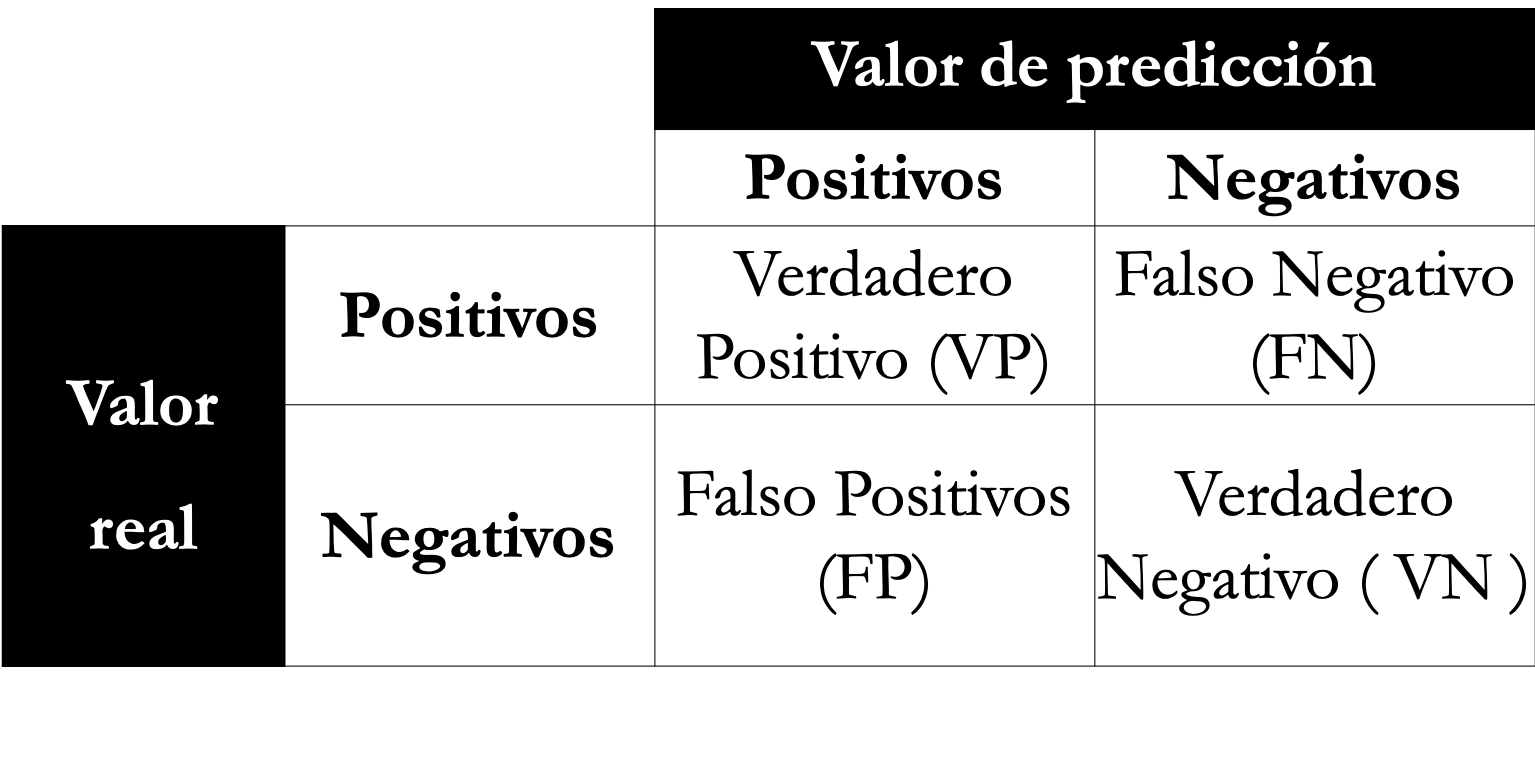
\includegraphics[scale=.45]{imagenes/Capitulo3/MatrizC.png}
	\caption{Matriz de confusión}
	\label{Fig:mconfu}
\end{figure}

La Figura \ref{Fig:mconfu} muestra un ejemplo de matriz de confusión con dos clases, la cual ejemplifica de
manera adecuada las diferentes entradas de la misma, entra las que se encuentran:


\begin{itemize}

	\item \textbf{VP}: Es la cantidad de datos positivos que fueron clasificados correctamente como positivos 
	\item \textbf{FN}: Es la cantidad de datos positivos que fueron clasificados incorrectamente como negativos
	\item \textbf{VN}: Es la cantidad de datos negativos que fueron clasificados correctamente como negativos
	\item \textbf{FP}: Es la cantidad de datos negativos que fueron clasificados incorrectamente como positivos
	
\end{itemize}

La diagonal principal en cualquier matriz de confusión n x n representa el número de predicciones
correctas para cada una de las n secciones.\\

Gracias a la matriz de confusión, es posible obtener ciertas métricas que nos ayudan a evaluar el modelo
de aprendizaje. Entre las que se encuentran:\\


\textbf{Exactitud}: es la proporción del número total de predicciones que son correctas respecto al total.
Se determina utilizando la ecuación:

\begin{equation}\label{eq:1}
	Exactitud = \frac{VP+VN}{VP+VN+FN+FP}
\end{equation}

\textbf{Recall}: Es la proporción de predicciones positivas que fueron correctamente clasificadas. Se determina
utilizando la ecuación:


\begin{equation}\label{eq:2}
	Recall = \frac{VP}{VP+FP}
\end{equation}


\textbf{Precisión}: Es la proporción de predicciones positivas que se clasificaron correctamente. Se determina
con la siguiente ecuación:


\begin{equation}\label{eq:3}
	Precision = \frac{VP}{VP+FN}
\end{equation}


\textbf{F-Measure (F1)}: Se interpreta como la media armónica entre Precisión y Recall. Se determina
con la siguiente ecuación:

\begin{equation}\label{eq:3}
	 F-Measure = 2 \cdot \frac{precision \cdot recall}{precision+recall}
\end{equation}

%------------------------------------

\Tlabel{cp3:validacionc}
\section{Validación cruzada}
\HSection{VALIDACÓN CRUZADA}

El proceso de validación cruzada es uno de los métodos mas usados para generalizar la capacidad de predecir de un modelo clasificador y para prevenir el sobre\-entrenamiento, ademas es usado en la etapa de entrenamiento de un algoritmo de aprendizaje supervisado \citep{CTValidacionC}. Este método consiste en dividir el corpus en $n$ pliegues como se muestra en la Figura \ref{cp3:diagramacv}, cada pliegue está conformado por \textbf{Dobleces} los cuales definen un conjunto de entrenamiento (doblez de color azul cielo) y otro de prueba (doblez de color azul rey). En cada pliegue se entrena el modelo y se prueba, para calcular la exactitud de este conjunto, al terminar el proceso se obtiene el promedio.\\

El objetivo de la validación cruzada es estimar la exactitud del modelo en nuevos datos. Cabe destacar que esta prueba permite encontrar un resultado más robusto y confiable en cuanto a la eficiencia del algoritmo, ya que asegura que los datos no sean manipulados para entrenar y probar con un conjunto de datos a conveniencia (es decir la combinación de información con la exactitud más alta).

%Daniel Berrar, in Encyclopedia of Bioinformatics and Computational Biology, 2019

\begin{figure}[h]
\centering
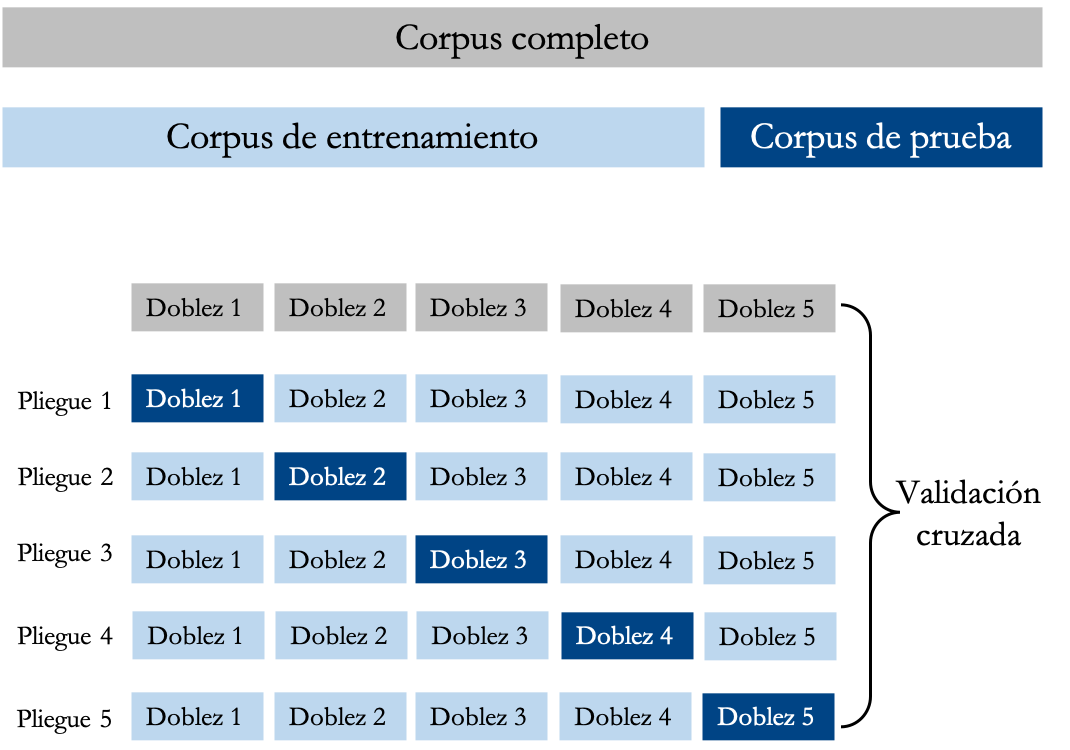
\includegraphics[scale=.75]{imagenes/Capitulo3/validacionc.png}
\caption{Validación cruzada}
\label{cp3:diagramacv}
\end{figure}


\newpage
%-------------------Recolección de información de Internet------------------------------------%
%---------------------------------------------------------------------------------------------%
\newpage
%\HNSection%--- Se normaliza el header---%

\MTtitle{Recolección de información de Internet} 

%-------------------------------Web Scraping----------------------------------------------%

\section{Web Scraping}

La recopilación de datos de Internet es una técnica que se realiza de manera manual, sin embargo 
el \textit{Web Scraping} es el conjunto de técnicas utilizadas para obtener de manera automática información de 
un sitio web \citep{CTWebScraping}. 
%El objetivo del Web Scraping es buscar cierto tipo de información definida y agregarla a nuevas páginas web. 
\\
El \textit{Web scraping} accede a las páginas web, encuentra los elementos de datos especificados en la 
página, los extrae y transforma en diferentes formatos si es necesario, finalmente, guarda 
la información como un conjunto de datos estructurado\footnote{Un conjunto de datos estructurado permite recolectar 
varios valores simultáneamente.}. Los investigadores limpian y organizan el contenido para analizar la información.

%------------------------Técnicas de Web Scraping----------------------------------------------%

\subsection{Técnicas de web scraping}

Algunas de las técnicas que nos proporciona el \textit{Web scraping} son\citep{CTTechniques}:

\begin{itemize}

    \item \textbf{Copiar y pegar}: Realiza el método recolección copiar y pegar la información, 
    sin embargo es una técnica propensa a errores

    \item \textbf{Uso de expresiones regulares}: Es una técnica que se puede utilizar para obtener la información 
    de las páginas web son las expresiones regulares, aunque comúnmente no se recomienda utilizarlas para parsear el formato HTML

    \item \textbf{Reconocimiento de anotaciones semánticas}: Las páginas que contienen metadatos, 
    marcas semánticas o explicaciones adicionales que se pueden usar para encontrar fragmentos de datos específicos

    \item \textbf{Parsers de HTML}: Algunos lenguajes, como XQuery y HTQL pueden ser utilizados para parsear documentos, recuperar 
    y transformar el contenido de documentos HTML

\end{itemize}

En el presente trabajo se hará uso de la técnica de \textbf{expresiones regulares}.\\
La Figura \textbf{\ref{fig:procesos}} muestra los procesos.

\begin{figure}[H]
    \centering
    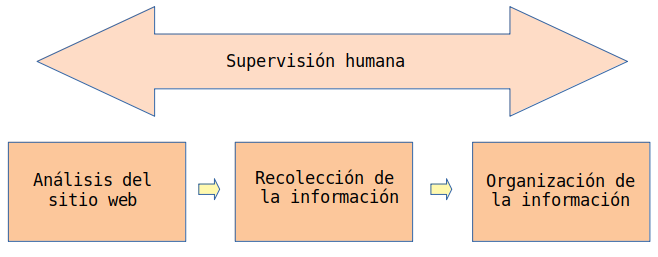
\includegraphics[scale=.35]{imagenes/Capitulo3/procesos}
    \caption{Etapas del proceso de \textit{Web scraping}.}
    \label{fig:procesos}
  \end{figure}
  
%--------------------------------Crawler---------------------------------------------%

\section{Crawler}
\Tlabel{c3:crawler}
Un \textit{Crawler}  es una herramienta la cual analiza sitios web, permitiendo recolectar 
las páginas web para así posteriormente extraer la información que contengan \citep{CTCrawler}. Un crawler también 
conocido como como robot o spider, es un sistema para la descarga masiva de páginas web. Son uno de 
los componentes principales de los motores de búsqueda web, los sistemas que reúnen un conjunto de 
páginas web, las indexan y permiten a los usuarios realizar consultas contra el índice y encontrar las 
sitios que coincidan con las consultas.

%--------------------------------Python---------------------------------------------%

\section{Python}
\textit{Python}\footnote{http://www.python.org/} un lenguaje de programación creado en 1991, se ha convertido en uno de los más 
importantes lenguajes de programación para la ciencia de datos, el aprendizaje automático y el desarrollo general de software en 
el mundo académico y la industria. 
En los últimos años, el soporte mejorado de Python para bibliotecas (como pandas y scikit-learn) lo ha convertido en una opción popular 
para las tareas de análisis de datos. Combinado con la solidez general de Python para la ingeniería de software de propósito general, 
es una excelente opción como idioma principal para crear aplicaciones de datos \citep{CTPython}.

%--------------------------------Scrapy---------------------------------------------%

\subsection{Scrapy}
\textit{Scrapy} es un \textit{framework} para rastrear sitios web y extraer datos estructurados que pueden utilizarse para una amplia 
gama de aplicaciones útiles, como la extracción de datos, el procesamiento de información o el archivo histórico.
A pesar de que Scrapy fue diseñado originalmente para el \textit{Web scraping}, también se puede usar para extraer datos mediante 
API (como los Servicios web de Amazon Associates) \citep{CTScrapy}.\\

La arquitectura del proyecto Scrapy se basa en arañas, que son rastreadores independientes que reciben un conjunto de instrucciones,
hace que sea más fácil construir y escalar grandes proyectos de \textit{Crawler} al permitir que los desarrolladores reutilicen su 
código. Scrapy también proporciona un una terminal de rastreo web, que los desarrolladores pueden usar para probar sus suposiciones 
sobre el comportamiento de un sitio.

%------------------------------------Aplicación web-------------------------------------------%
%---------------------------------------------------------------------------------------------%
\newpage
\MTtitle{Aplicación web}

%--------------------------------------Internet--------------------------------------------%

\section{Internet}

Son muchas las definiciones que se encuentran de la Internet, sin embargo su definición es simple, 
``la Internet es una colección de redes de comunicación interconectadas mediante el protocolos 
lo cual lo cual garantiza que las redes físicas que la componen, formen una red lógica única de 
alcance mundial'' \citep{CTInternet}.
\\

Uno de los principales objetivos cuando se desarrolló fue permitir la comunicación entre distintos usuarios,
hoy en día es utilizado para muchos ámbitos, desde obtener información relevante, hasta comprar artículos 
provenientes de otros países.
\\

El Instituto Nacional de Estadística y Geografía (INEGI) realizó una encuesta\footnote{https://www.inegi.org.mx/programas/dutih/2018/}  
en donde se muestra que al año 2018 hay 18.3 millones de hogares que disponen de Internet, es decir más del 
50\% de la población en México.
El acceso a Internet ha crecido de manera exponencial, permitiendo a los usuarios tener infresar a distintos recursos.

%se puede enviar y reciibir información al mismo tiempo y a través de las mismas rutas de comunicación.

%------------------------------------World Wide Web--------------------------------------------%

\subsection{World Wide Web}

La WWW \textit{World Wide Web} es un sistema de distribución de documentos HTML \textit{HyperText Markup Language} 
que permite a los usuarios de computadora ejecutar aplicaciones basadas en Web, además de localizar y ver documentos 
basados en multimedia sobre casi cualquier tema a través de Internet.
La \textit{World Wide Web} es una colección gigante de documentos o páginas, almacenados en computadoras de todo el mundo. 
Comúnmente llamada la Web, esta colección de páginas representa una gran cantidad de texto, imágenes, audio y video disponibles 
para cualquier persona con una computadora y una conexión a Internet.

%--------------------------------------HTML-------------------------------------------%
\Tlabel{cp3:html}
\section[HTML]{Hypertext markup language}
HyperText Markup Language (\textit{HTML}, por sus siglas en ingles), 
es un lenguaje que permite presentar contenido en la Web y fue propuesto por primera vez por 
Tim Berners-Lee (1989). El estándar ha evolucinado continuamente desde su introducción inicial, 
la versión más reciente es HTML5 que está siendo desarrollada por el \textit{World Wide Web Consurtium} (W3C).
\\
Un archivo HTML es un texto sin formato, el cual se puede abrir y editar con cualquier editor de 
texto. Lo que hace al HTML tan poderoso es su estructura marcada, el cual permite definir las partes 
de un documento que deben mostrarse como titulares, las partes que contienen enlaces, las partes que deben 
organizarse como tablas y muchas otras formas. Las definiciones de marcado se basan en secuencias de caracteres 
predefinidas, las etiquetas, que encierran partes del texto \citep{CTHTML}. 

%--------------------------------------Sitios web------------------------------------------%

\section{Sitios web}
Un sitio web es un conjunto de páginas web relacionadas entre sí. Se entiende por página web tanto el fichero 
que contiene el código HTML como todos los recursos que se emplean en la página, como pueden ser
imágenes sonidos, videos \citep{CTsW}.
Un sitio web son de acceso público que comparten un solo nombre de dominio, pueden ser creados y 
mantenidos por un individuo, grupo, empresa u organización para cumplir una variedad de propósitos. 
Todos estos sitios constituyen la World Wide Web. 

%---------------------------------------Página web------------------------------------------%

\subsection{Página web}

Una página web es un documento electrónico el cual forma parte de la WWW (\textit{World Wide Web}) generalmente 
construido en el lenguaje HTML (\textit{Hyper Text Markup Language}). Este documento puede contener enlaces que nos 
direcciona a otra página web. Para visualizar una página web es necesario de un browser o un navegador. 
Dentro de las páginas web se encuentra un sinfin de sitios los cuales pueden ser de interés. 
Las páginas web pueden ser estáticas o dinámicas. Las páginas estáticas muestran el mismo contenido cada vez que se 
visualizan. Las páginas dinámicas tienen contenido que puede cambiar cada vez que se accede a ellas \citep{CTpW}. 

%-------------------------------------------Blog------------------------------------------%

\subsection{Blog}

Un blog es una página web en la cual el usuario no necesita conocimientos específicos del medio electrónico ni del 
formato digital para poder aportar contenidos de forma inmediata, ágil y constante desde cualquier punto de conexión 
a Internet \citep{CT17}. \\
Un blog es un sitio web que generalmente contiene información realizada por un autor. Esta información pueden ser de varios 
tipos, como comentarios, descripciones de eventos, fotos, videos, comentarios personales, tutoriales, estudios de casos, artículos 
de opinión extensos, ideas políticas o cualquier otra cosa que pueda imaginar. Por lo general, se muestran en orden cronológico 
inverso, con las adiciones más recientes en la parte superior. Esas entradas de información se pueden organizar de varias maneras, por fecha, tema. 
Una de las características principales de un blog es que se debe actualizar periódicamente. A diferencia de un sitio web donde el 
contenido es estático, un blog se comporta más como un diario en línea, donde el blogger publica actualizaciones periódicas. Por lo 
tanto, los blogs son dinámicos con contenido siempre cambiante. Un blog se puede actualizar con contenido nuevo y el contenido anterior se 
puede cambiar o eliminar en cualquier momento (aunque eliminar el contenido no es una práctica común) \citep{CTBlog}.

%----------------------------------------------Foro-----------------------------------------%

\subsection{Foro}

Un foro es una herramienta de comunicación asíncrona. Los foros permiten la comunicación de los participantes desde 
cualquier lugar en el que  esté  disponible  una  conexión  a Internet  sin  que  éstos  tengan  que  estar dentro del 
sistema al mismo tiempo, de ahí su naturaleza asíncrona. Brindando una mayor interacción entre distintos 
participantes y permitiendo conocer la opinión sobre un tema de distintas personas.
Los foros son probablemente el único recurso de resolución de problemas y recursos basados en información en la Internet, 
le brindan un entorno interactivo en el que puede aprender y apliar sus conocimientos \citep{CTForum}.


  \newpage
  \TChapter{Análisis y diseño}{delta}
\ \\\\
En este capítulo se describe el análisis y el diseño del sistema web para el trabajo terminal propuesto, mostrando los módulos con los cual cuenta. Hasta este punto se presentan los requisitos que deberá cumplir el sistema así como los casos de uso y diagramas de secuencia.

\section{Actores y roles}
Usuario: Cualquier persona que ingrese al sistema y esté interesada en consultar noticias.


%------------------------Requisitos Funcionales ------------------%
\section[Requisitos f.]{Requisitos funcionales}

%----------------------------RF1------------------------------%
   \Dline{RF1}{Recolectar noticias}
    \begin{itemize}
      \item \textbf{Descripción:} El sistema debe recolectar noticias de forma automática de los sitios web definidos.\\
    \end{itemize}
%----------------------------RF2------------------------------%
   \Dline{RF2}{Clasificar noticias}
    \begin{itemize}
      \item \textbf{Descripción:} El sistema debe clasificar las noticias recolectadas de acuerdo a su contenido, en las secciones previamente definidas.\\
    \end{itemize}
%----------------------------RF3------------------------------%
    \Dline{RF3}{Filtrar noticias}
    \begin{itemize}
      \item \textbf{Descripción:} El sistema debe filtrar las noticias recolectadas de acuerdo a la fecha de publicación; el periodo permitido para el filtrado 
      de noticias es: de la fecha actual de ingreso al sistema hasta tres días antes. Cabe destacar que de encontrar noticias anteriores a este periodo, estas podrán ser visualizadas.\\
    \end{itemize}
%----------------------------RF4------------------------------%
   \Dline{RF4}{Mostrar resultados}
    \begin{itemize}
      \item \textbf{Descripción:} El sistema debe mostrar las noticias que cumplan con los filtros de búsqueda establecidos por el usuario 
      (Sección y fecha de publicación).\\
    \end{itemize}


%------------------------Requisitos No Funcionales ---------------%
\section[Requisitos no f.]{Requisitos no funcionales}



%----------------------------RNF1------------------------------%
   \DVline{RNF1}{Tiempo de recolección y clasificación}
    \begin{itemize}
      \item \textbf{Descripción:} El tiempo de recolección y clasificación de las noticias no debe tomar mas de 1 minuto.\\
    \end{itemize}

%----------------------------RNF2------------------------------%
   \DVline{RNF2}{Número de palabras}
    \begin{itemize}
     \item \textbf{Descripción:} Las noticias recolectadas deben tener un mínimo de 180 palabras en ellas.\\
    \end{itemize}
 %Argumenar   

%----------------------------RNF3------------------------------%  
   \DVline{RNF3}{Número de noticias mostradas}
    \begin{itemize}
      \item \textbf{Descripción:} El sistema debe mostrar al menos 5 noticias clasificadas, por página.\\
    \end{itemize}
%Justificar con un promedio de las noticias que muestran los sitios web en cada sección



%----------------------------Reglas de negocio---------------------%  
\section{Reglas de negocio}


En esta sección se describen las reglas de negocio implementadas en el trabajo propuesto.\\\\


%------------------RN1-----------------------%
\DGline{RN1}{Número de palabras}
\begin{itemize}
  \item \textbf{Descripción:}  La noticia debe tener al menos 180 palabras.
%  \item \textbf{Ejemplo:}
  \item \textbf{Referenciado por}: \Tref{CU1}{CU1 Recolectar noticias}
\end{itemize}

%------------------RN2-----------------------%
\DGline{RN2}{Lenguaje de noticias}

\begin{itemize}
  \item \textbf{Descripción:} Las noticias deben estar redactadas en lenguaje español.
%  \item \textbf{Ejemplo:}
  \item \textbf{Referenciado por: CU2 Clasificar noticias}  \\
\end{itemize}
%------------------RN3-----------------------%
\DGline{RN3}{Listado de fuentes noticiosas}

\begin{itemize}
  \item \textbf{Descripción:} Solo se puede recolectar información de los siguientes sitios.\\

  \begin{itemize}

    \item \textbf{El Universal}: https://www.eluniversal.com.mx/
    \item \textbf{Azteca Noticias}: https://www.aztecanoticias.com.mx/
    \item \textbf{Aristegui Noticias}: https://aristeguinoticias.com/
    \item \textbf{La Jornada}: https://www.jornada.com.mx/ultimas
    \item \textbf{Sopitas}: https://www.sopitas.com/
    \item \textbf{El Economista}: https://www.eleconomista.com.mx/
    \item \textbf{Proceso}: https://www.proceso.com.mx/

  \end{itemize} 
%  \item \textbf{Ejemplo:}
  \item \textbf{Referenciado por}: \Tref{CU1}{CU1 Recolectar noticias} \\
\end{itemize}
%------------------RN4-----------------------%
%\DGline{RN4}{Umbral de grado de pertenencia}
%
%\begin{itemize}
%  \item \textbf{Descripción:} Solo se puede mostrar una noticia si su grado de pertenencia a una %sección es mayor o igual al umbral establecido.%
%%  \item \textbf{Ejemplo:}%
%  \item \textbf{Referenciado por: CU2 Clasificar noticias}  \\
%\end{itemize}

%------------------RN4-----------------------%
\DGline{RN4}{Número de noticias recolectadas}

\begin{itemize}
  \item \textbf{Descripción:} El número máximo de noticias recolectadas por sitio web debe ser 30.

%  \item \textbf{Ejemplo:}%
  \item \textbf{Referenciado por}:\Tref{CU1}{CU1 Recolectar noticias}  \\
\end{itemize}

%------------------RN5-----------------------%
\DGline{RN5}{Orden de publicación}

\begin{itemize}
  \item \textbf{Descripción:} Las noticias se muestran con base a la fecha de publicación.
%  \item \textbf{Ejemplo:} 
  \item \textbf{Referenciado por}: \Tref{CU1}{CU1 Recolectar noticias},\Tref{CU4}{CU4 Mostrar resultados} \\
\end{itemize}

%------------------RN6----------------------%
\DGline{RN6}{Periodo de recolección}

\begin{itemize}
  \item \textbf{Descripción:} De cada sitio establecido se recolectan las noticias que se encuentren en un periodo de al menos 3 días anterior a la fecha actual.
  \item \textbf{Referenciado por}: \Tref{CU1}{CU1 Recolectar noticias} \\
\end{itemize}

%------------------RN7----------------------%
\DGline{RN7}{Campos recolectados de noticia}

\begin{itemize}
  \item \textbf{Descripción:} De cada noticia se extrae \textbf{Título}, \textbf{URL al artículo}, \textbf{Fecha de publicación} y de contar con ello el \textbf{Resumen}.

  \item \textbf{Referenciado por}: \Tref{CU1}{CU1 Recolectar noticias}\\
\end{itemize}


%------------------RN8----------------------%
\DGline{RN8}{Periodo de actualización}

\begin{itemize}
  \item \textbf{Descripción:} El proceso de recolección de noticias se hará en periodos de 4 horas 

  \item \textbf{Referenciado por}: \Tref{CU1}{CU1 Recolectar noticias}\\
\end{itemize}


%--------------------------Casos de uso -------------------------%

\newpage
\section{Casos de uso}

%--------------------------Diagrama CU -------------------------%
\Tsubsection{Diagrama de casos de uso}



La Figura \textbf{\ref{fig:DCU}} muestra el diagrama de casos de uso de la aplicación. Los casos de uso marcados en color gris son descritos en el documento, mientras que los mostrados en color rojo serán desarrollados en trabajo terminal II.

\begin{figure}[h]
  \centering
  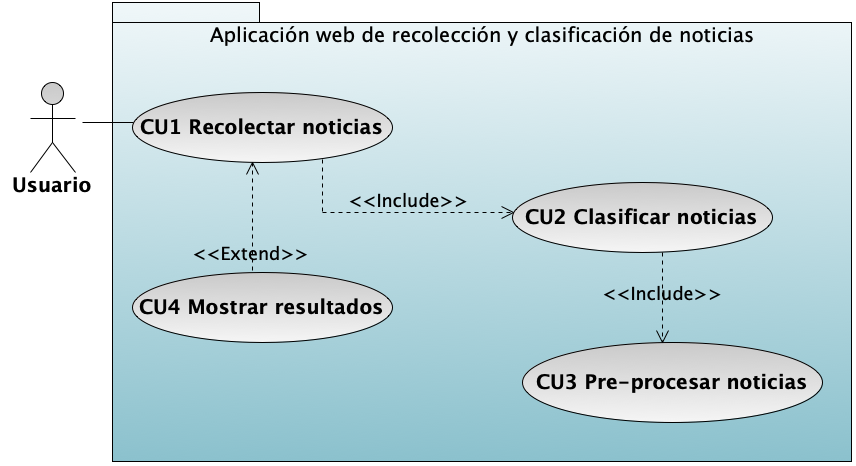
\includegraphics[scale=.4]{imagenes/Diagramas/CasosDeuso/CasosDeuso}
  \caption{Diagrama de casos de uso}
  \label{fig:DCU}
\end{figure}

\newpage


  \newpage
  \Tlabel{CU1}\Tsubsection{CU1 Recolectar noticias}

%================================Intriodcucción==================================%
%----------------------Resumen-----------------------------------%
\begin{large}
	\textbf{Resumen}\\
\end{large}

Brinda al usuario un punto de acceso para elegir una sección; las clasificaciones son, \textbf{Ciencia y tecnología}, \textbf{Política}, \textbf{Deportes}, \textbf{Economía} y  \textbf{Cultura}, posteriormente se recolectan noticias de la web, tomando como punto de partida los sitios establecidos previamente. De cada sitio se recolectan las noticias publicadas; de cada artículo se obtiene \textbf{Fecha de publicación}, \textbf{Título}, \textbf{Contenido}, \textbf{URL de la noticia}, y de contar con ello el \textbf{Resumen}.\\

\begin{large}
	\textbf{Descripción}\\
\end{large} 

%=====================================Tabla 1====================================%


\begin{tabular}{|l|l|}
%-----------------------Ecanbezado-----------------------------------%
	\hline
	\multicolumn{1}{| >{\columncolor{black}}l|}{ \textcolor{myWhite}{\textbf{Caso de uso: }} }&
	\multicolumn{1}{| >{\columncolor{black}}l|}{ \textcolor{myWhite}{CU1 Recolectar noticias} }\\
	\hline
%-----------------------Actor----------------------------------------%
	\textbf{Actor:} & 	Usuario\\
	\hline

%-----------------------Propósito------------------------------------%

	\textbf{Propósito:} & Brindar una herramienta de recolección de noticias\\
	& de Internet(Crawler) \\
	\hline

%----------------------Entradas--------------------------------------%

	\textbf{Entradas:} & URL de las paginas por consultar\\
	\hline

%-----------------------Salidas--------------------------------------%

	\textbf{Salidas:} & \Tref{MSG1}{MSG1 Tiempo de recolección excedido}\\
	\hline

%-----------------------Precondiciones-------------------------------%

	\textbf{Precondición:} & Tener un punto de conexión a Internet\\
	\hline
%-----------------------Postcondiciones------------------------------%

	\textbf{Postcondiciones:} &$\bullet$  El usuario tendrá la facultad\\
	&\ \  de visualizar las noticias clasificadas\\
	&$\bullet$ El usuario podrá cambiar el periodo de búsqueda\\
	\hline

	%-----------------------Reglas de negocio----------------------------%

	\textbf{Reglas de negocio:} &$\bullet$ \RNref{RN1}{Número de palabras}\\
	&$\bullet$ \RNref{RN3}{Listado de fuentes noticiosas}\\
	&$\bullet$ \RNref{RN5}{Orden de publicación}\\
	&$\bullet$ \RNref{RN6}{Periodo de recolección}\\
	&$\bullet$ \RNref{RN7}{Campos recolectados de noticia}\\
	&$\bullet$ \RNref{RN8}{Periodo de actualización}\\
	\hline

%---------------------------Errores----------------------------------%

%------Error 1----------%
	\textbf{Errores:} & $\bullet$ \TError{CU1}{Uno} Cuando el tiempo de \\
	&\ \ recolección se ha excedido se muestra el mensaje\\
	&\ \  \Tref{MSG1}{MSG1 Tiempo de recolección excedido}\\
	\hline

\end{tabular}

\ \\\\

%============================Trayectorias========================================%

%-----------------------Trayectoria Principal-----------------------%


\begin{large}
	\textbf{Trayectoria principal}\\
\end{large}	

\begin{enumerate}[1.]

	
	\item \actor Selecciona una opción de la pantalla \Tref{UI1}{UI1 Inicio}; \textbf{Política}, \textbf{Economía}, \textbf{Deportes}, \textbf{Ciencia y tecnología} o \textbf{Cultura}. 

	\item \sistema Verifica que no existan noticias recolectadas previamente. \TAref{CU1}{A}

	\item \sistema \label{CU1:Recolectar}Muestra la pantalla \Tref{UI2}{Pantalla UI2 Espera de proceso}. 

	\item \sistema Por cada sitio se extraen las noticias con base en la regla de negocio {RN3}{Listado de fuentes noticiosas}, \RNref{RN6}{Periodo de recolección} y \RNref{RN7}{Campos recolectados de noticia.} \TAref{CU1}{D}

	\item \label{CU1:BuscarN}\sistema Incluye el caso de uso \textbf{CU2 Clasificar noticias}.

	\item \sistema \label{CU1:NoticiasR} Se obtienen las noticias clasificadas de la sección seleccionada por el usuario, de acuerdo a la regla de negocio \RNref{RN5}{Orden de publicación.}

	\item \sistema Muestra la pantalla \Tref{UI3}{Pantalla UI3 Proceso concluido}.

	\item \finCU	

\end{enumerate}







%-------------------------trayectoria Alternativa A-----------------%
\begin{large}
	\Talterna{CU1}{A}\\
\end{large}	
\textbf{Condición:} \textit{Existen noticias recolectadas}

\begin{enumerate}[{A-}1.]

	\item \sistema Verifica que la última recolección de noticias no exceda el periodo establecido, con base \RNref{RN8}{Periodo de actualización}.

	\item \actor Continua en el paso \ref{CU1:NoticiasR} de la trayectoria principal.

	\item \finTA

\end{enumerate}

%-------------------------trayectoria Alternativa B-----------------%
\begin{large}
	\Talterna{CU1}{B}\\
\end{large}	
\textbf{Condición:} \textit{La última recolección de noticias excede el periodo establecido}

\begin{enumerate}[{B-}1.]

	\item \actor Continua en el paso \ref{CU1:Recolectar} de la trayectoria principal.

	\item \finTA

\end{enumerate}


%================================Puntos de extención=============================%


\begin{large}
	\textbf{Puntos de extensión}\\
\end{large}	

%--------------------Puntos de extención 1------------------------%
\textbf{Causa de la extensión:} El usuario desea consultar las noticias clasificadas.\\
\textbf{Región de la trayectoria:} Proviene del paso \ref{CU1:NoticiasR} de la trayectoria principal.\\
\textbf{Extiende a :} \Tref{CU4}{CU4 Mostrar resultados}\\\\



  \newpage
  \Tlabel{CU4}\Tsubsection{CU4 Mostrar resultados}

%================================Intriodcucción==================================%
%----------------------Resumen-----------------------------------%

\begin{large}
	\textbf{Resumen}\\
\end{large}

Permite al actor visualizar las noticias correspondiente a la sección elegida, ya sea \textbf{Política}, \textbf{Deportes}, \textbf{Ciencia y tecnología}, \textbf{Economía} o \textbf{Cultura}. Cada artículo contiene el \textbf{Título}, \textbf{Autor}, la \textbf{Fecha de publicación}, \textbf{URL} el cual direcciona a la página fuente que ha proporcionado la noticias y de contar con ello un \textbf{Resumen de la noticia}. Además se permite filtrar las noticias en un periodo de al menos tres días. Cabe destacar que las noticias mostradas por defecto, corresponden a la fecha actual.\\

\begin{large}
	\textbf{Descripción}\\
\end{large}



%=====================================Tabla 1====================================%
\begin{table}[H]
	\centering
	\begin{tabular}{|l|l|}

	%-----------------------Ecanbezado-----------------------------------%
		\hline
		\multicolumn{1}{| >{\columncolor{black}}l|}{ \textcolor{myWhite}{\textbf{Caso de uso: }} }&
		\multicolumn{1}{| >{\columncolor{black}}l|}{ \textcolor{myWhite}{CU4 Mostrar resultados} }\\
		\hline
	%-----------------------Actor----------------------------------------%
		\textbf{Actor:} & 	Usuario	\\
		\hline
	%-----------------------Propósito------------------------------------%
		\textbf{Propósito:} & Brindar una herramienta que permita consultar las\\
		&noticias clasificadas y filtradas por su fecha de publicación\\
		\hline

	%----------------------Entradas--------------------------------------%
		\textbf{Entradas:} &Periodo de búsqueda\\
		\hline

	%-----------------------Salidas--------------------------------------%
		\textbf{Salidas:}&$\bullet$ \Tref{MSG2}{MSG2 Petición vacía}\\
		&$\bullet$ Noticias clasificadas; de cada una se muestra:\\
		&\ \ $\circ$ \textbf{Título}\\
		&\ \ $\circ$ \textbf{URL al artículo}\\
		&\ \ $\circ$ \textbf{Fecha de publicación}\\
		&\ \ $\circ$ \textbf{Autor}\\
		&\ \ $\circ$ \textbf{Resumen}\\
		\hline

	%-----------------------Precondiciones-------------------------------%

		\textbf{Precondición:} & Las noticias clasificadas deben estar \\
		&almacenadas por sección\\
		\hline

	%-----------------------Postcondiciones------------------------------%

	%---------Post 1----------%
		\textbf{Postcondiciones:}& Ninguna\\
		\hline

	%-----------------------Reglas de negocio----------------------------%
		\textbf{Reglas de negocio:}& \RNref{RN5}{Orden de publicación}\\
		\hline
	%---------------------------Errores----------------------------------%

	%------Error 1----------%
		\textbf{Errores:} &\TError{CU4}{Uno} Cuando no se ha encontrado noticias en el\\
		&\ \ día seleccionado se muestra el mensaje \Tref{MSG2}{MSG2}\\
		&\ \ \Tref{MSG2}{Petición vacía}\\
		\hline

	\end{tabular}

	%\caption{ Tabla de descripción de CU4 }
\end{table}
%============================Trayectorias========================================%

%-----------------------Trayectoria Principal-----------------------%

\begin{large}
	\textbf{Trayectoria principal}\\
\end{large}	

\begin{enumerate}[1.]

	\item \actor Presiona el botón \textbf{Continuar} de la pantalla \Tref{UI3}{Pantalla UI3 Proceso concluido}. \TAref{CU1}{A}

	\item \sistema Obtiene la fecha actual.

	\item \sistema Muestra al menos 5 noticias, de acuerdo a la regla de negocio \RNref{RN5}{Orden de publicación} de la sección previamente elegida (filtro de sección) y del día actual (filtro de fecha), como se visualiza en la pantalla \Tref{UI4}{UI4 Resultados de consulta}.

	\item \actor \label{CU4:Consulta}Consulta la noticia.\TAref{CU4}{B}

	\item \finCU	
\end{enumerate}


%-------------------------trayectoria Alternativa A-----------------%
\begin{large}
	\Talterna{CU4}{A}\\
\end{large}	
\textbf{Condición:} \textit{El usuario ha presionado el botón cancelar}

\begin{enumerate}[{A-}1.]

	\item \actor Presiona el botón \textbf{Cancelar} de la pantalla \Tref{UI3}{Pantalla UI3 Proceso concluido}.

	\item \sistema Muestra la pantalla \Tref{UI1}{UI1 Inicio}.

	\item \finTA

\end{enumerate}


%-------------------------trayectoria Alternativa B-----------------%
\begin{large}
	\Talterna{CU4}{B}\\
\end{large}	
\textbf{Condición:} \textit{El usuario ha cambiado el periodo establecido}

\begin{enumerate}[{B-}1.]

	\item \actor \label{CU4:Dia}Presiona un botón del menú \textbf{Cambio de periodo} de la pantalla \Tref{UI4}{UI4 Resultados de consulta}.

	\item \sistema Verifica que exista al menos 1 noticia en el periodo establecido. \TAref{CU4}{C}

	\item \sistema Muestra noticias de acuerdo a la regla de negocio \RNref{RN5}{Orden de publicación} de la sección previamente elegida (filtro de sección) y del día seleccionado en el paso \ref{CU4:Dia} (filtro de fecha), como se visualiza en la pantalla \Tref{UI5}{UI5 Cambio de periodo}.

	\item \sistema Continua en el paso \ref{CU4:Consulta} de la trayectoria principal.

	\item \finTA

\end{enumerate}


%-------------------------trayectoria Alternativa C-----------------%
\begin{large}
	\Talterna{CU4}{C}\\
\end{large}	
\textbf{Condición:} \textit{No se ha encontrado noticias del día seleccionado \TEref{CU4}{Uno}}

\begin{enumerate}[{C-}1.]

	\item \sistema Muestra el mensaje \Tref{MSG2}{MSG2 Petición vacía}, en la pantalla \Tref{UI4}{UI4 Resultados de consulta}.

	\item \sistema Continua en el paso \ref{CU4:Consulta} de la trayectoria principal.

	\item \finTA

\end{enumerate}


  \newpage

%------------------------Mensajes----------------------------------%

\section{Mensajes}
  
  %------------------MSG1-----------------------%
     \Mline{MSG1}{Tiempo de recolección excedido}
    \begin{itemize}
      \item \textbf{Tipo:} Error. 
      \item \textbf{Objetivo:}  Dar a conocer que se ha excedido el tiempo de recolección de noticias de los sitios web definidos.
      \item \textbf{Redacción:} Se ha agotado el tiempo de espera, no se han encontrado noticias. Intentar más tarde.
      \item \textbf{Referenciado por:} \Tref{CU1}{CU1 Recolectar noticias}\\
    \end{itemize}

  %------------------MSG2-----------------------%
   \Mline{MSG2}{Petición vacía}
  \begin{itemize}
    \item \textbf{Tipo:} Error. 
    \item \textbf{Objetivo:}  Informar al usuario que no se ha encontrado resultados en el día seleccionado.
    \item \textbf{Redacción:}  No se ha encontrado noticias en el día seleccionado.

    \item \textbf{Referenciado por:} \Tref{CU4}{CU4 Mostrar resultados}\\
  \end{itemize}

  %------------------MSG3-----------------------%
   \Mline{MSG3}{Fallo en la recolección}
  \begin{itemize}
    \item \textbf{Tipo:} Error. 
    \item \textbf{Objetivo:}  Informar al usuario que las ligas registradas en el diccionario de \textbf{URLs} no permiten extraer información.
    \item \textbf{Redacción:} No se puede extraer noticias de los sitios registrados en este portal web.
    \item \textbf{Referenciado por:} \Tref{CU1}{CU1 Recolectar noticias}\\
  \end{itemize}

  %------------------MSG4-----------------------%
%   \Mline{MSG4}{Fallo al ingresar a sitio web}
%  \begin{itemize}
%    \item \textbf{Tipo:} Error. 
%    \item \textbf{Objetivo:} Informar al usuario sobre el fallo ocurrido en la conexión del portal web seleccionado.
%    \item \textbf{Redacción:} Ha ocurrido un fallo en la conexión con el sitio seleccionado, intente mas tarde.
%    \item \textbf{Referenciado por:} \Tref{CU7}{CU7 Ingresar a sitio web}\\
%  \end{itemize}

\newpage

  %--------------------------Descripción de pantallas ------------------%
\section{Pantallas}

\Tsubsection{UI1 Página de inicio} 
%------------------------------------Objetivo----------------------------------%
\begin{large}
  \textbf{Objetivo}\\
\end{large}


Permite al usuario seleccionar la sección a consultar.\\

%------------------------------------Descripción---------------------------------%
\begin{large}
  \textbf{Descripción}\\
\end{large}

La Pantalla \ref{fig:UI1} muestra un menú con las secciones definidas para el sistema las cuales son: \textbf{Política}, \textbf{Deportes}, \textbf{Ciencia y tecnología}, \textbf{Economía} y \textbf{Cultura}. En ella se puede navegar para acceder a la consulta de las noticias recolectadas y clasificadas de alguna sección.\\

%-----------------------------------Salidas------------------------------------%
\begin{large}
  \textbf{Salidas}
\end{large}

\begin{itemize}

  \item \Tref{MSG2}{MSG2 Tiempo de recolección excedido}

\end{itemize}

%------------------------------------Comandos----------------------------------%

\textbf{Comandos}

\begin{enumerate}

  \item \textbf{Inicio}: Direcciona a la pantalla descrita en esta sección
  \item \textbf{Política}: Permite realizar una consulta en la sección Política
  \item \textbf{Deportes}: Permite realizar una consulta en la sección Deportes
  \item \textbf{Ciencia y tecnología}: Permite realizar una consulta en la sección Ciencia
  \item \textbf{Economía}: Permite realizar una consulta en la sección Economía
  \item \textbf{Cultura}: Permite realizar una consulta en la sección Cultura

\end{enumerate}

%------------------------------------Referencia----------------------------------%
\begin{large}
  \textbf{Referenciado por}
\end{large}

\begin{itemize}

  \item \Tref{CU1}{CU1 Recolectar noticias}
  \item \Tref{CU4}{CU4 Mostrar resultados}

\end{itemize}  

%----------------------------------------Pantalla--------------------------------%

\begin{figure}\Tlabel{UI1}
  \centering
	
\includegraphics[scale=.35]{imagenes/Pantallas/UI1}
  \caption{Pantalla UI1 Inicio}
  \label{fig:UI1}
\end{figure}



\Tsubsection{UI2 Recolección y clasificación} 
%------------------------------------Objetivo----------------------------------%
\begin{large}
  \textbf{Objetivo}\\
\end{large}


Informar al usuario que la recolección y clasificación de noticias se está llevando acabo.\\

%------------------------------------Descripción---------------------------------%
\begin{large}
  \textbf{Descripción}\\
\end{large}

La Pantalla \ref{fig:UI2} muestra un mensaje flotante con la siguiente redacción: \textbf{En proceso de recolección y clasificación}, para informar al usuario que la consulta realizada está en proceso.\\

%-----------------------------------Salidas------------------------------------%
\begin{large}
  \textbf{Salidas}
\end{large}

\begin{itemize}

  \item Ninguno

\end{itemize}

%------------------------------------Comandos----------------------------------%


%------------------------------------Referencia----------------------------------%
\begin{large}
  \textbf{Referenciado por}
\end{large}

\begin{itemize}

  \item \Tref{CU1}{CU1 Recolectar noticias}

\end{itemize}  

%----------------------------------------Pantalla--------------------------------%


\begin{figure}\Tlabel{UI2}
  \centering 
	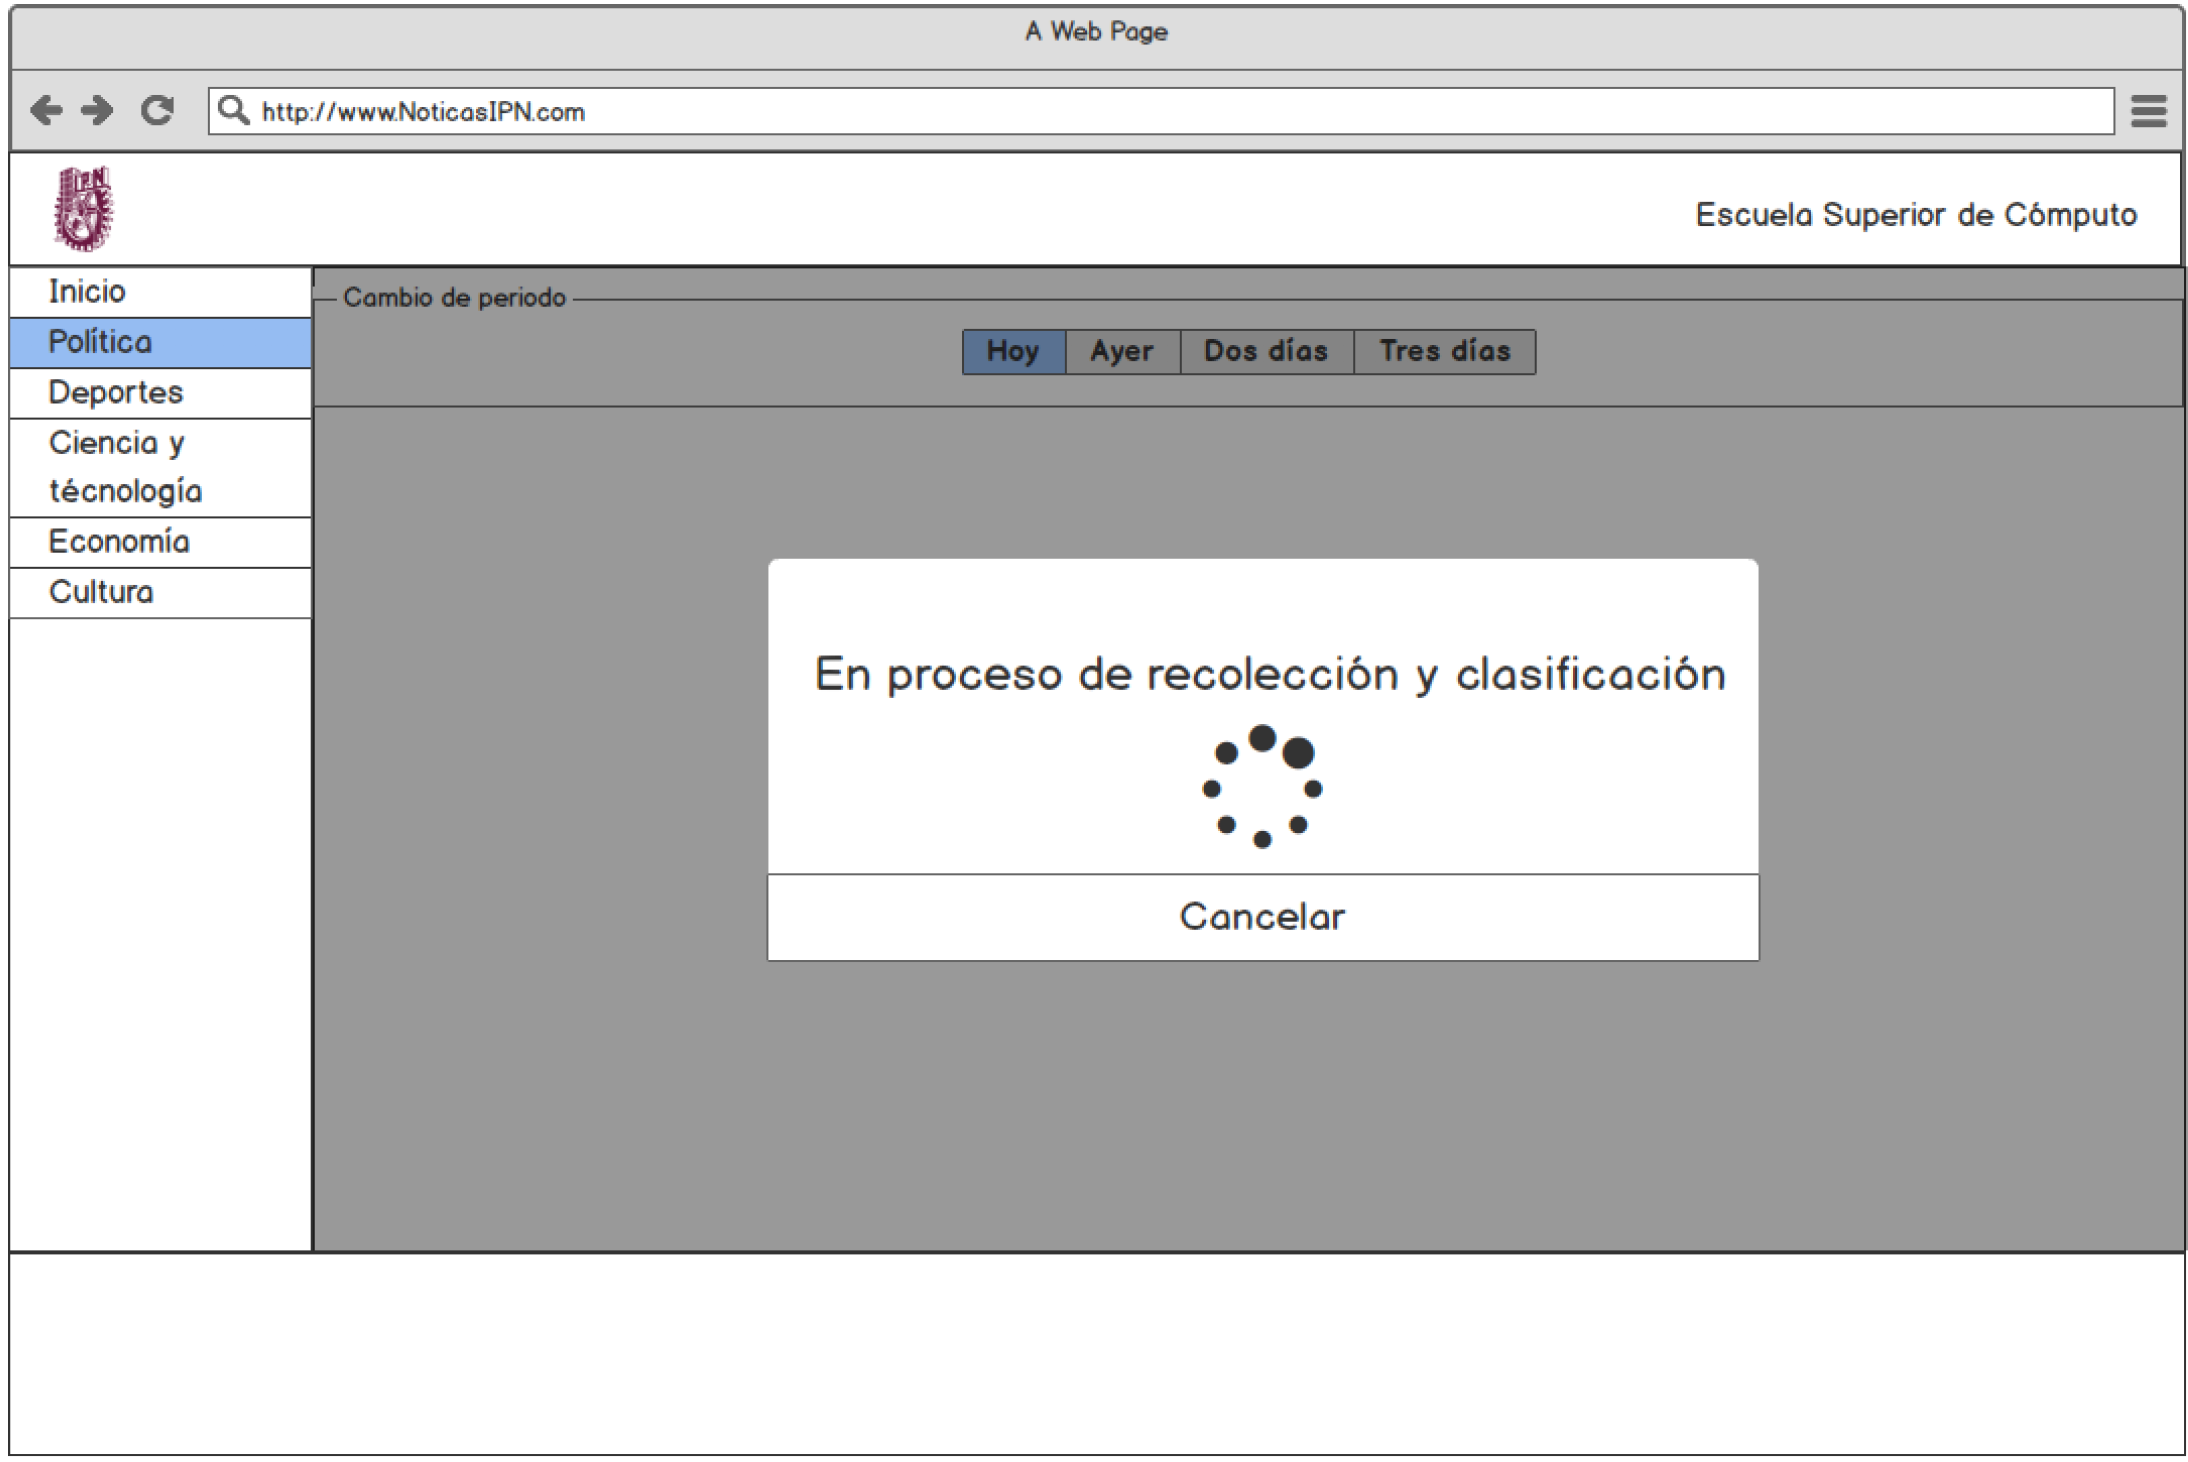
\includegraphics[scale=.32]{imagenes/Pantallas/UI2}
  \caption{Pantalla UI2 Espera de proceso}
  \label{fig:UI2}
\end{figure}

\Tsubsection{UI3 Proceso concluido} 
%------------------------------------Objetivo----------------------------------%
\begin{large}
  \textbf{Objetivo}\\
\end{large}


Informal al usuario que la recolección y clasificación ha concluido y brinda un punto de acceso para visualizar los resultados de la consulta.\\

%------------------------------------Descripción---------------------------------%
\begin{large}
  \textbf{Descripción}\\
\end{large}

La Pantalla \ref{fig:UI3} muestra un mensaje flotante con la siguiente redacción: \textbf{Noticias listas para ser mostradas}, el cual informa al usuario que el proceso de recolección y clasificación ha concluido, \textit{i.e} ya se pueden mostrar las noticias clasificadas de la sección elegida. En la parte inferior se muestra el botón \textbf{Cancelar} y \textbf{Continuar}.  \\

%-----------------------------------Salidas------------------------------------%
\begin{large}
  \textbf{Salidas}
\end{large}

\begin{itemize}

  \item Ninguno

\end{itemize}

%------------------------------------Comandos----------------------------------%

\textbf{Comandos}

\begin{enumerate}

  \item \textbf{Cancelar}: Detiene el proceso de recolección y clasificación, re-direcciona a la pantalla \Tref{UI1}{UI1 Inicio}.
  \item \textbf{Continuar}: Permite avanzar para visualizar las noticias clasificadas de la sección elegida en la pantalla \Tref{UI4}{UI4 Resultados de consulta}

\end{enumerate}

%------------------------------------Referencia----------------------------------%
\begin{large}
  \textbf{Referenciado por}
\end{large}

\begin{itemize}

  \item \Tref{CU1}{CU1 Recolectar noticias}
  \item \Tref{CU4}{CU4 Mostrar resultados}

\end{itemize}  

%----------------------------------------Pantalla--------------------------------%

\begin{figure}\Tlabel{UI3}
  \centering
	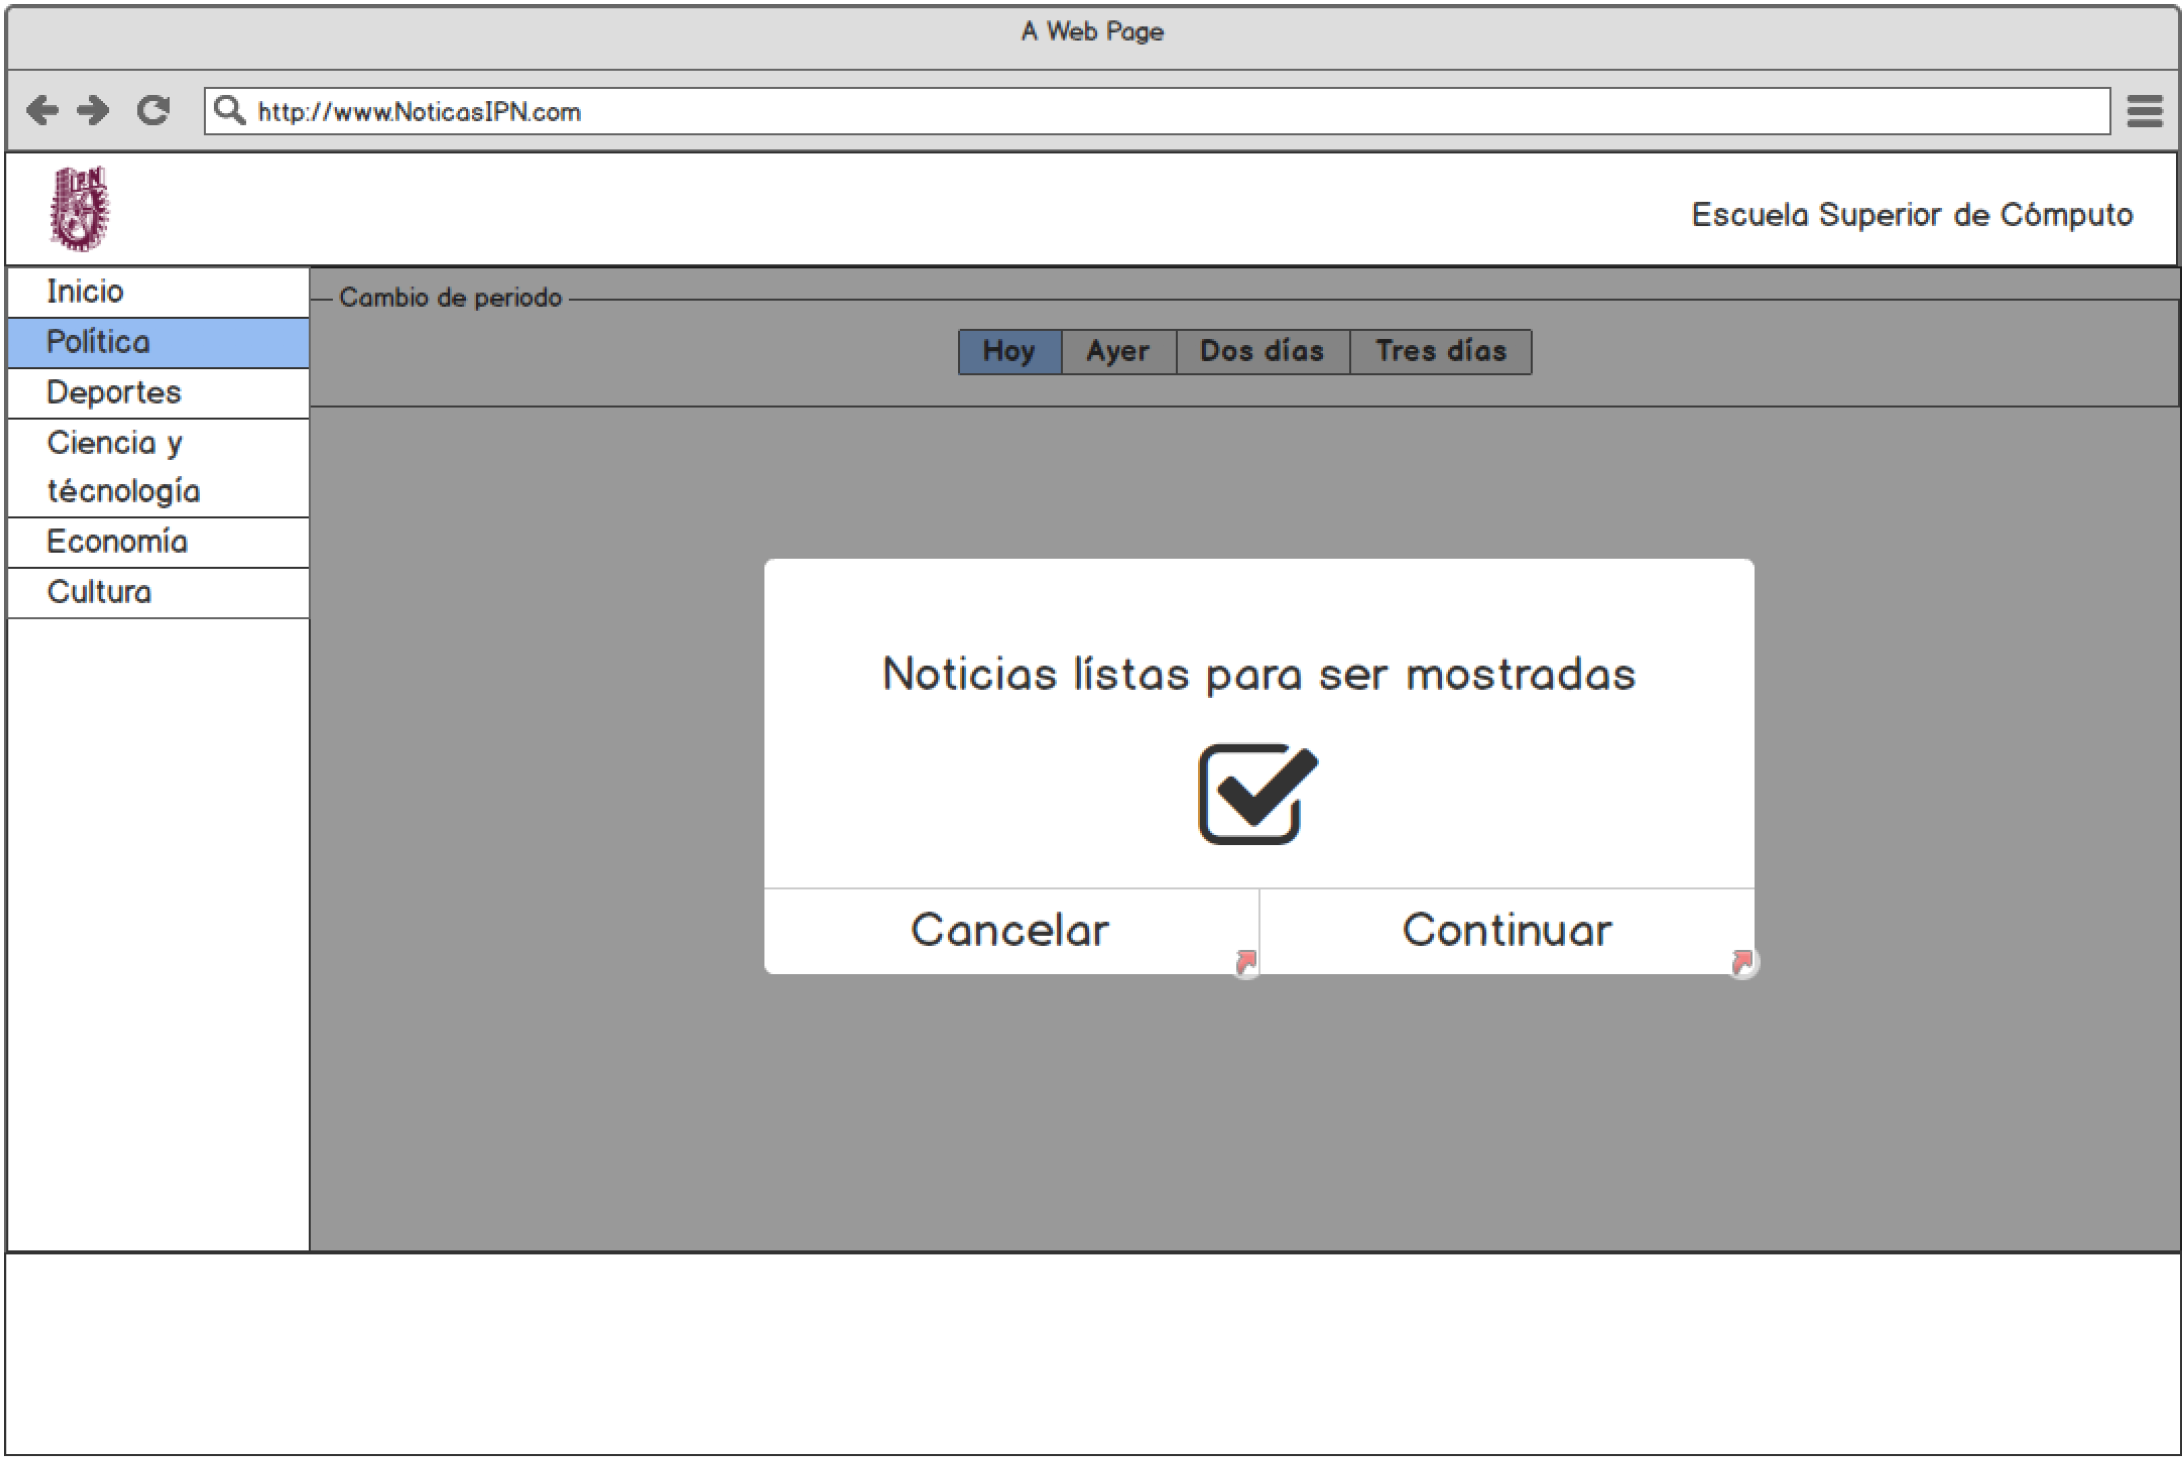
\includegraphics[scale=.35]{imagenes/Pantallas/UI3}
  \caption{Pantalla UI3 Proceso concluido}
  \label{fig:UI3}
\end{figure}

\Tsubsection{UI4 Resultados de consulta} 
%------------------------------------Objetivo----------------------------------%
\begin{large}
  \textbf{Objetivo}\\
\end{large}


Permite consultar las noticias clasificadas en la sección previamente elegida. Además brinda una forma de cambiar el periodo de búsqueda y permite entrar al sitio de origen de los artículos mostrados.\\

%------------------------------------Descripción---------------------------------%
\begin{large}
  \textbf{Descripción}\\
\end{large}

La Pantalla \ref{fig:UI4} muestra una sección con las noticias clasificadas, de cada noticia se muestra:

\begin{itemize}

  \item \textbf{Título}
  \item \textbf{URL al artículo}
  \item \textbf{Fecha de publicación}
  \item \textbf{Resumen}

\end{itemize}

En la parte superior de la pantalla se muestra el menú \textbf{Cambio de periodo} el cual permite cambiar le periodo de consulta de las noticias. Cabe señalar que la primera vez que se ingresa a esta pantalla se muestran los artículos con fecha de publicación del día actual.
La Pantalla \ref{fig:UI5} muestra un ejemplo de consulta en una fecha diferente.



%-----------------------------------Salidas------------------------------------%
\begin{large}
  \textbf{Salidas}
\end{large}

\begin{itemize}

  \item \Tref{MSG2}{MSG2 Petición vacía}

\end{itemize}

%------------------------------------Comandos----------------------------------%

\textbf{Comandos}

\begin{enumerate}

  \item \textbf{Hoy}: Realiza la consulta en la fecha actual
  \item \textbf{Ayer}: Realiza la consulta un día antes de la fecha actual
  \item \textbf{Dos días}: Realiza la consulta dos días antes de la fecha actual
  \item \textbf{Tres días}: Realiza la consulta tres días antes de la fecha actual
  \item \textbf{URL}: La url que muestra la noticia direcciona al sitio web de recolección


\end{enumerate}

%------------------------------------Referencia----------------------------------%
\begin{large}
  \textbf{Referenciado por}
\end{large}

\begin{itemize}

  \item \Tref{CU4}{CU4 Mostrar resultados}

\end{itemize}  

%----------------------------------------Pantalla--------------------------------%


%-----------------------------UI1--------------------------%
\begin{figure}\Tlabel{UI4}
  \centering
  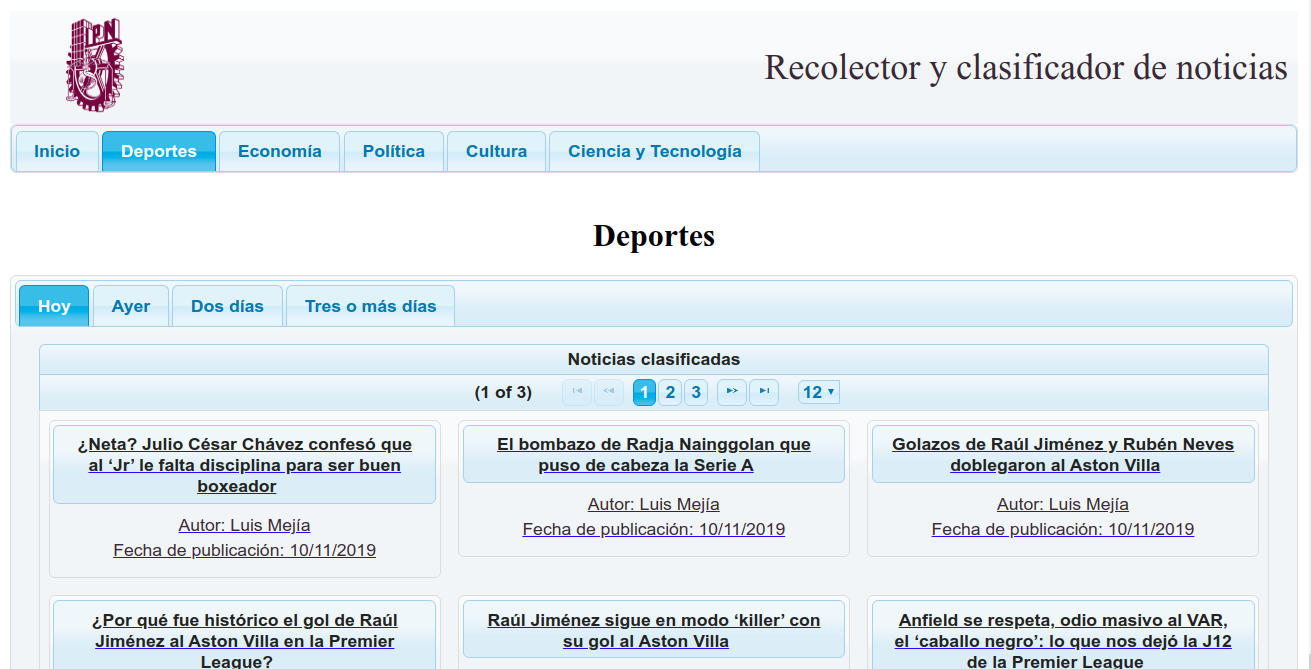
\includegraphics[scale=.32]{imagenes/Pantallas/UI4}
  \caption{Pantalla UI4 Resultados de consulta}
  \label{fig:UI4}
\end{figure}

%-----------------------------UI2--------------------------%
\begin{figure}\Tlabel{UI5}
  \centering
  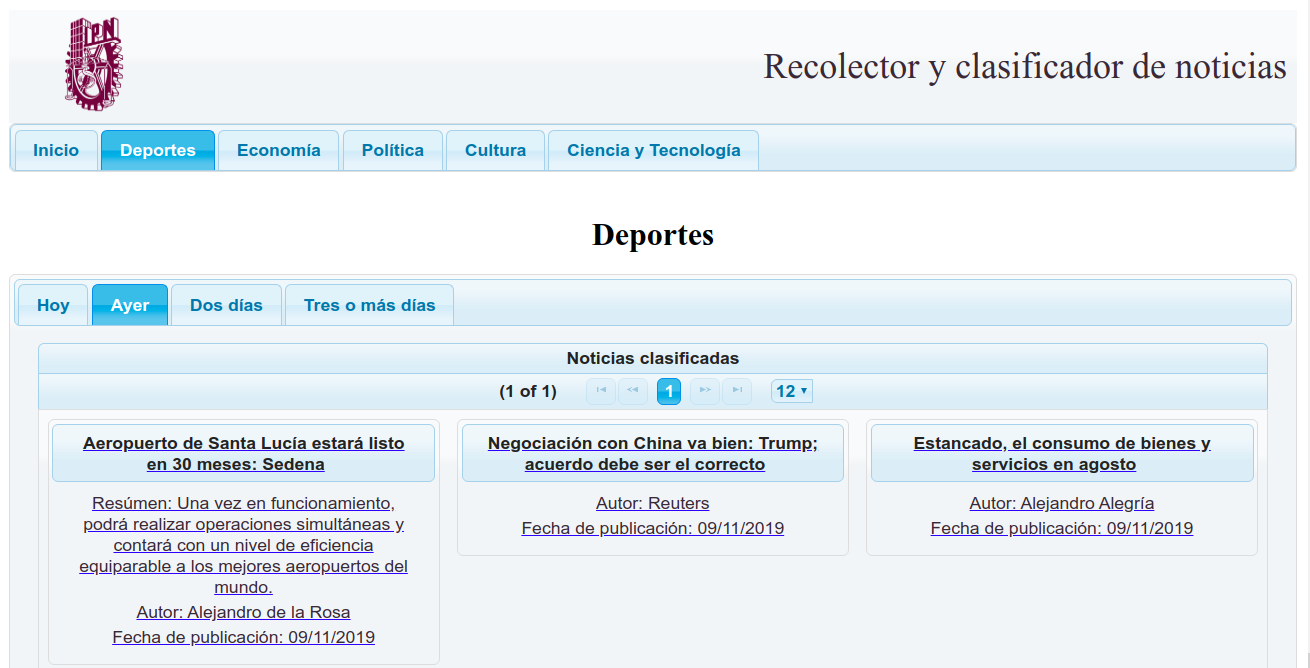
\includegraphics[scale=.32]{imagenes/Pantallas/UI5}
  \caption{Pantalla UI5 Cambio de periodo}
  \label{fig:UI5}
\end{figure}



\newpage


%-------------------------------Diagrama de secuencia

\section{Diagrama de secuencia}




La figura \textbf{\ref{fig:DSE}} muestra el diagrama de secuencia de la aplicación. 

\begin{figure}[H]
  \centering
  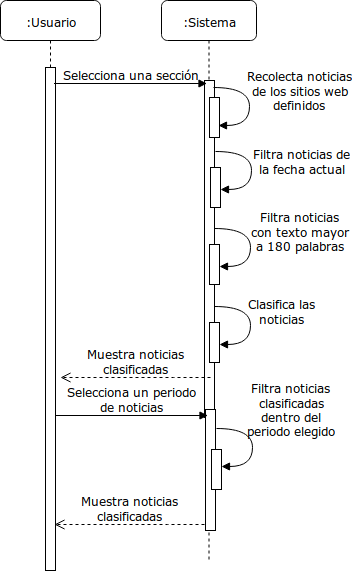
\includegraphics[scale=.75]{imagenes/Diagramas/Secuencia/Diagrama}
  \caption{Diagrama de secuencia}
  \label{fig:DSE}
\end{figure}

\newpage


  \newpage
   \TChapter{Avances}{epsilon}
\ \\\\
En esta sección se mostrarán los avances que hasta el día de hoy se tienen.

%-----------------------------------------------------------------------------------------%
\section{Herramientas utilizadas}
Para el desarrollo de los avances en el presente trabajo, se utilizó el lenguaje de programación Python\footnote{https://www.python.org/} 
en la distribución Anaconda\footnote{https://www.anaconda.com/distribution/}, ya que gestiona las 
versiones de las librerías utilizadas para el análisis de datos, y para el recolector web (Crawler) se utilizó Scrapy\footnote{https://scrapy.org/}, 
un framework que permite la extracción de información de sitios web.

%-----------------------------------------------------------------------------------------%

\section{Estudio previo}
Una vez elegidas las herramientas que permiten la extracción de la información, se procedió con la selección de los 
sitios web para extraer noticias.
\\
El sitio web El Economista\footnote{https://www.eleconomista.com.mx/} contiene una sección llamada 
\textbf{Ranking de Medios Nativos Digitales}\footnote{https://www.eleconomista.com.mx/Ranking-de-Medios-Nativos-Digitales}, 
el cual muestra las estadísticas que realiza mes con mes acerca de los sitios de noticias web más consultados como se muestra 
en la Figura \textbf{\ref{fig:rank}}
\begin{figure}[H]
  \centering
  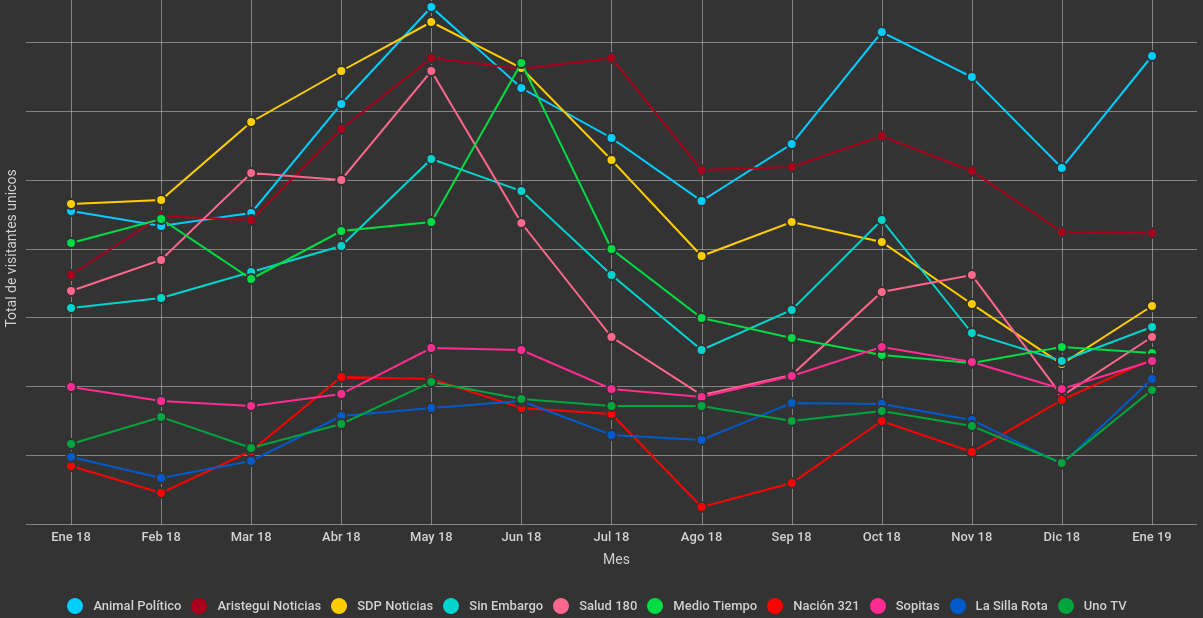
\includegraphics[scale=.28]{imagenes/Capitulo5/ranking}
  \caption{Ranking de sitios de noticias del periódo de enero del 2018 a enero del 2019.}
  \label{fig:rank}
\end{figure}
 

Para la selección final de los sitios de noticias que se utilizarán en estre trabajo, se revisaron los los medios mostrados en la Figura 5.1. Después de esta revisión se encontró que los sitios Salud 180 y Medio Tiempo muestran noticias relacionadas únicamente con salud y deportes respectivamente. En este trabajo se desean obtener noticias de diversas secciones por lo que estos sitios se descartaron. También para este trabajo es importante incluir información de otros medios como diarios y  sitios de televisón, por lo tanto se incluyeron sitios relacionados con estos medios.

\begin{itemize}
    \item 3 Sitios de foros de noticias: 
    \begin{itemize}
      \item \textbf{Aristegui Noticias}: https://aristeguinoticias.com/
      \item \textbf{SDP Noticias}: https://www.sdpnoticias.com/
      \item \textbf{Sopitas}: https://www.sopitas.com/
    \end{itemize}
    \item 3 Sitios de diarios:
    \begin{itemize}
      \item \textbf{El Universal}: https://www.eluniversal.com.mx/
      \item \textbf{La Jornada}: https://www.jornada.com.mx/
      \item \textbf{Exélsior}: https://www.excelsior.com.mx/
    \end{itemize}
    \item 3 Sitios de televisión:
    \begin{itemize}
      \item \textbf{TV Azteca}: https://www.aztecanoticias.com.mx/
      \item \textbf{Televisa}: https://noticieros.televisa.com/
      \item \textbf{Once Noticias}: https://www.oncenoticias.tv/
    \end{itemize}
\end{itemize}

Los sitios organizan las noticias en secciones. Una vez seleccionados los sitios, se procedió con el análisis de las secciones que contienen los portales, como 
lo muestra la Tabla \textbf{\ref{tabla:sitios}}.

\begin{table}[htbp]
    \centering
    \resizebox{\columnwidth}{!}{%
    \begin{tabular}[H]{|l|l|l|l|l|l|l|l|l|}


 \multicolumn{1}{| >{\columncolor{myBlueChapter}}l|}{ \textcolor{myWhite}{\textbf{El}} }
&\multicolumn{1}{| >{\columncolor{myBlueChapter}}l|}{ \textcolor{myWhite}{\textbf{La}} }
&\multicolumn{1}{| >{\columncolor{myBlueChapter}}l|}{ \textcolor{myWhite}{\textbf{Milenio}} }
&\multicolumn{1}{| >{\columncolor{myBlueChapter}}l|}{ \textcolor{myWhite}{\textbf{Aristegui}} }
&\multicolumn{1}{| >{\columncolor{myBlueChapter}}l|}{ \textcolor{myWhite}{\textbf{SDP}} }
&\multicolumn{1}{| >{\columncolor{myBlueChapter}}l|}{ \textcolor{myWhite}{\textbf{Sopitas}} }
&\multicolumn{1}{| >{\columncolor{myBlueChapter}}l|}{ \textcolor{myWhite}{\textbf{Azteca}} }
&\multicolumn{1}{| >{\columncolor{myBlueChapter}}l|}{ \textcolor{myWhite}{\textbf{Televisa}} }
&\multicolumn{1}{| >{\columncolor{myBlueChapter}}l|}{ \textcolor{myWhite}{\textbf{Once}} }
  \\ \cline{1-9}
%---------------------------------------------------------------------------------------%

 \multicolumn{1}{| >{\columncolor{myBlueChapter}}l|}{ \textcolor{myWhite}{\textbf{Universal}} }
&\multicolumn{1}{| >{\columncolor{myBlueChapter}}l|}{ \textcolor{myWhite}{\textbf{Jornada}} }
&\multicolumn{1}{| >{\columncolor{myBlueChapter}}l|}{ }
&\multicolumn{1}{| >{\columncolor{myBlueChapter}}l|}{ \textcolor{myWhite}{\textbf{Noticias}} }
&\multicolumn{1}{| >{\columncolor{myBlueChapter}}l|}{ \textcolor{myWhite}{\textbf{Noticias}} }
&\multicolumn{1}{| >{\columncolor{myBlueChapter}}l|}{ }
&\multicolumn{1}{| >{\columncolor{myBlueChapter}}l|}{ \textcolor{myWhite}{\textbf{Noticias}} }
&\multicolumn{1}{| >{\columncolor{myBlueChapter}}l|}{ }
&\multicolumn{1}{| >{\columncolor{myBlueChapter}}l|}{ \textcolor{myWhite}{\textbf{Noticias}} }
\\ \cline{1-9}

%---------------------------------------------------------------------------------------%

        Nacional      & -            & Nacional      & México                & Nacional      & Noticias  & -                 & Nacional      & Nacional      \\ 
        \hline
%---------------------------------------------------------------------------------------%

       	Mundo         & Mundo        & Mundo         & Destacado o       & Internacional & -         & Internacional     & Internacional & Internacional \\ 
        & & & Mundo & & & & & \\ 
        \hline
%---------------------------------------------------------------------------------------%

        Metrópoli     & Capital      & CDMX          & -                     & -             & -         & -                 & CDMX          & CDMX      \\ 
        \hline
%---------------------------------------------------------------------------------------%

        Estados       & Estados      & Estados       & Sociedad o       & Estados       & -         & Estados           & Estados       & Nacional   \\ 
        & & & México & & & & & \\ 
        \hline
%---------------------------------------------------------------------------------------%

        Cartera       & Economía     & Negocios      & Economía              & Economía      & -         & Finanzas          & Economía      & Economía   \\ 
        \hline
%---------------------------------------------------------------------------------------%

        Deportes      & Deportes     & La Afición    & Deportes              & Deportes      & Deportes  & -                 & Deportes      & Deportes   \\ 
        \hline
%---------------------------------------------------------------------------------------%

        Espectáculos  & Espectáculos & Hey           & -                     & En el show    & Entretenimiento & -           & Entretenimiento & Deportes    \\ 
        \hline
%---------------------------------------------------------------------------------------%

        Cultura       & Cultura      & Cultura       & -                     & -             & -         & -                 & Arte y cultura & Cultura   \\ 
        \hline
%---------------------------------------------------------------------------------------%

        Nación o & Política   & Política      & Poderes               & -             & -         & Política          & Política      & -   \\ 
        & política & & & & & & & \\ 
        \hline
%---------------------------------------------------------------------------------------%

        Ciencia y & Tecnología & Tecnología    &                       & Geek          & Geek      & -                 & Tecnología*      & Ciencia\\
        salud & & & & & & & & \\ 
        \hline        

    \end{tabular}%
}
\caption[Tabla]{Secciones existentes en los sitios web}
\label{tabla:sitios}
\end{table}

Una vez que se analizarón las secciones con las que contaba cada sitio se procedió a homologar las secciones en las cuales la mayoría de los sitios coincidian, por lo cual se quedarón definidas 5 secciones para clasificación de las noticia:

\begin{itemize}
    \item Política
    \item Deportes
    \item Ciencia y tecnología
    \item Economía
    \item Cultura
\end{itemize}

Para llevar a cabo el proceso de extracción de las noticias, se realizó el estudio 
de la estructura XML (\textit{Extensible Markup Language}), por sus siglas en inglés de cada sitio web seleccionado, con 
el objetivo de definir las etiquetas que poseen la información de las noticias, las cuales son:

\begin{itemize}
  \item URL
  \item Sección
  \item Título
  \item Autor
  \item Fecha
  \item Descripción
  \item Noticia
\end{itemize} 

%-----------------------------------------------------------------------------------------%
\section{Recolección de noticias}
En la siguiente Figura \textbf{\ref{fig:diagrama}}. se describe el proceso de recolección:

\begin{figure}[H]
  \centering
  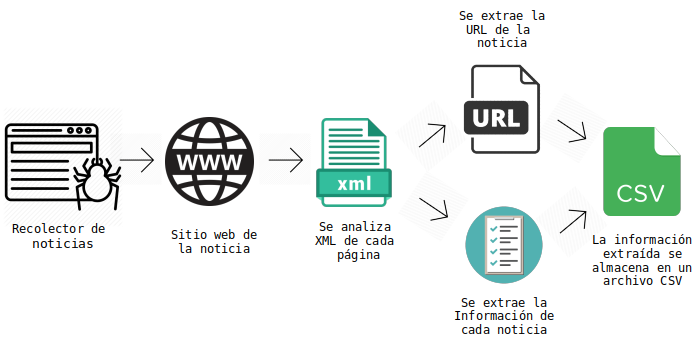
\includegraphics[scale=.50]{imagenes/Capitulo5/diagrama}
  \caption{Proceso de recolección de noticias.}
  \label{fig:diagrama}
\end{figure}

%-----------------------------------------------------------------------------------------%
\subsection{Desarrollo}

Con base en la información obtenida de los sitios web, se diseño un recolector de noticias para cada sitio, procede con 
los siguientes pasos para realizar la extracción de noticias.

\begin{itemize}
  \item Se ingresa a la URL definida como inicio y se analiza la etiqueta definida que redirecciona a cada noticia del sitio web
  \item Una vez que se ha ingresado a la noticia se procede con el análisis de las etiquetas definidas
  \item Se extrae la información de cada noticia, así como su URL
  \item Posteriormente la información recolectada se guarda en un archivo csv
\end{itemize}
La siguiente figura muestra el comando que realiza el proceso de recolección de las noticias.

%Para el proceso de extracción se abre una terminal con la ruta donde se guardará la información recolectada Figura \textbf{\ref{fig:uno}} 
%Se va a redactar los pasos del proceso de recolección

%-----------------------------------------------------------------------------------------%
\subsection{Resultados}

%-----------------------------------------------------------------------------------------%
\subsubsection{Secciones recolectadas}

De los nueve sitios web definidos se obtuvieros las siguientes secciones mostrados en la Tabla \textbf{\ref{tabla:secciones}}:
\\
\begin{table}[htbp]
  \centering
  \resizebox{\columnwidth}{!}{%
  \begin{tabular}{|c|c|c|c|c|c|c|c|c|c|}

 \multicolumn{1}{| >{\columncolor{myBlueChapter}}l|}{ \textcolor{myWhite}{\textbf{Sección}} }
&\multicolumn{1}{| >{\columncolor{myBlueChapter}}l|}{ \textcolor{myWhite}{\textbf{El}} }
&\multicolumn{1}{| >{\columncolor{myBlueChapter}}l|}{ \textcolor{myWhite}{\textbf{La}} }
&\multicolumn{1}{| >{\columncolor{myBlueChapter}}l|}{ \textcolor{myWhite}{\textbf{Milenio}} }
&\multicolumn{1}{| >{\columncolor{myBlueChapter}}l|}{ \textcolor{myWhite}{\textbf{Aristegui}} }
&\multicolumn{1}{| >{\columncolor{myBlueChapter}}l|}{ \textcolor{myWhite}{\textbf{SDP}} }
&\multicolumn{1}{| >{\columncolor{myBlueChapter}}l|}{ \textcolor{myWhite}{\textbf{Sopitas}} }
&\multicolumn{1}{| >{\columncolor{myBlueChapter}}l|}{ \textcolor{myWhite}{\textbf{Azteca}} }
&\multicolumn{1}{| >{\columncolor{myBlueChapter}}l|}{ \textcolor{myWhite}{\textbf{Televisa}} }
&\multicolumn{1}{| >{\columncolor{myBlueChapter}}l|}{ \textcolor{myWhite}{\textbf{Once}} }
  \\ \cline{1-10}
%---------------------------------------------------------------------------------------%
 \multicolumn{1}{| >{\columncolor{myBlueChapter}}l|}{ }
&\multicolumn{1}{| >{\columncolor{myBlueChapter}}l|}{ \textcolor{myWhite}{\textbf{Universal}} }
&\multicolumn{1}{| >{\columncolor{myBlueChapter}}l|}{ \textcolor{myWhite}{\textbf{Jornada}} }
&\multicolumn{1}{| >{\columncolor{myBlueChapter}}l|}{ }
&\multicolumn{1}{| >{\columncolor{myBlueChapter}}l|}{ \textcolor{myWhite}{\textbf{Noticias}} }
&\multicolumn{1}{| >{\columncolor{myBlueChapter}}l|}{ \textcolor{myWhite}{\textbf{Noticias}} }
&\multicolumn{1}{| >{\columncolor{myBlueChapter}}l|}{ }
&\multicolumn{1}{| >{\columncolor{myBlueChapter}}l|}{ \textcolor{myWhite}{\textbf{Noticias}} }
&\multicolumn{1}{| >{\columncolor{myBlueChapter}}l|}{ }
&\multicolumn{1}{| >{\columncolor{myBlueChapter}}l|}{ \textcolor{myWhite}{\textbf{Noticias}} }
\\ \cline{1-10}


  %---------------------------------Economía--------------------------------------%  
  Economía & \Checkmark & \Checkmark & \Checkmark & \Checkmark & \Checkmark & \XSolidBrush & \Checkmark & \Checkmark & \Checkmark \\
  \hline
  %-----------------------------------Deportes------------------------------------%  

  Deportes & \Checkmark & \Checkmark & \Checkmark & \Checkmark & \Checkmark & \Checkmark & \XSolidBrush & \Checkmark & \Checkmark \\
  \hline

  %-----------------------------------Cultura------------------------------------%  
  Cultura & \Checkmark & \Checkmark & \Checkmark & \XSolidBrush & \XSolidBrush & \XSolidBrush & \XSolidBrush & \Checkmark & \Checkmark \\
  \hline

  %-----------------------------------Política------------------------------------%  
  Política  & \Checkmark & \Checkmark & \Checkmark & \Checkmark & \XSolidBrush & \XSolidBrush & \Checkmark & \Checkmark & \XSolidBrush \\
  \hline

  %-------------------------------Ciencia y tecnología-----------------------------------%  
  Ciencia y& \Checkmark & \Checkmark & \Checkmark & \XSolidBrush & \Checkmark & \Checkmark & \XSolidBrush & \Checkmark & \Checkmark \\
  tecnología  & & & & & & & & & \\
  \hline

    \end{tabular}%
}
\caption{Secciones contenidas en los sitios web definidos}
\label{tabla:secciones}
\end{table}

%-----------------------------------------------------------------------------------------%
\subsubsection{Resultados de las etiquetas}
En la Tabla \textbf{\ref{tabla:etiquetas}}, muestra los campos que pueden ser extraídos por cada sitio.
%Expresar la idea de que se intento recolectar toda la información sin embargo no se pueo 
\begin{table}[htbp]
  \centering
  \resizebox{\columnwidth}{!}{%
  \begin{tabular}{|c|c|c|c|c|c|c|c|c|c|}

 \multicolumn{1}{| >{\columncolor{myBlueChapter}}l|}{ \textcolor{myWhite}{\textbf{Etiqueta}} }
&\multicolumn{1}{| >{\columncolor{myBlueChapter}}l|}{ \textcolor{myWhite}{\textbf{El}} }
&\multicolumn{1}{| >{\columncolor{myBlueChapter}}l|}{ \textcolor{myWhite}{\textbf{La}} }
&\multicolumn{1}{| >{\columncolor{myBlueChapter}}l|}{ \textcolor{myWhite}{\textbf{Milenio}} }
&\multicolumn{1}{| >{\columncolor{myBlueChapter}}l|}{ \textcolor{myWhite}{\textbf{Aristegui}} }
&\multicolumn{1}{| >{\columncolor{myBlueChapter}}l|}{ \textcolor{myWhite}{\textbf{SDP}} }
&\multicolumn{1}{| >{\columncolor{myBlueChapter}}l|}{ \textcolor{myWhite}{\textbf{Sopitas}} }
&\multicolumn{1}{| >{\columncolor{myBlueChapter}}l|}{ \textcolor{myWhite}{\textbf{Azteca}} }
&\multicolumn{1}{| >{\columncolor{myBlueChapter}}l|}{ \textcolor{myWhite}{\textbf{Televisa}} }
&\multicolumn{1}{| >{\columncolor{myBlueChapter}}l|}{ \textcolor{myWhite}{\textbf{Once}} }
  \\ \cline{1-10}
%---------------------------------------------------------------------------------------%
 \multicolumn{1}{| >{\columncolor{myBlueChapter}}l|}{ }
&\multicolumn{1}{| >{\columncolor{myBlueChapter}}l|}{ \textcolor{myWhite}{\textbf{Universal}} }
&\multicolumn{1}{| >{\columncolor{myBlueChapter}}l|}{ \textcolor{myWhite}{\textbf{Jornada}} }
&\multicolumn{1}{| >{\columncolor{myBlueChapter}}l|}{ }
&\multicolumn{1}{| >{\columncolor{myBlueChapter}}l|}{ \textcolor{myWhite}{\textbf{Noticias}} }
&\multicolumn{1}{| >{\columncolor{myBlueChapter}}l|}{ \textcolor{myWhite}{\textbf{Noticias}} }
&\multicolumn{1}{| >{\columncolor{myBlueChapter}}l|}{ }
&\multicolumn{1}{| >{\columncolor{myBlueChapter}}l|}{ \textcolor{myWhite}{\textbf{Noticias}} }
&\multicolumn{1}{| >{\columncolor{myBlueChapter}}l|}{ }
&\multicolumn{1}{| >{\columncolor{myBlueChapter}}l|}{ \textcolor{myWhite}{\textbf{Noticias}} }
\\ \cline{1-10}

  %-----------------------------------URL------------------------------------%  
      URL         & \Checkmark & \Checkmark & \Checkmark & \Checkmark & \Checkmark & \Checkmark & \Checkmark & \Checkmark & \Checkmark \\
      \hline

  %-----------------------------------Sección------------------------------------%  
      Sección     & \Checkmark & \Checkmark & \Checkmark & \Checkmark & \Checkmark & \Checkmark & \Checkmark & \Checkmark & \Checkmark \\ 
      \hline

  %-----------------------------------Título------------------------------------%  
      Título      & \Checkmark & \Checkmark & \Checkmark & \Checkmark & \Checkmark & \Checkmark & \Checkmark & \Checkmark & \Checkmark \\ 
      \hline

  %----------------------------------Autor-----------------------------------%  
      Autor       & \Checkmark & \Checkmark & \Checkmark & \Checkmark & \Checkmark & \Checkmark & \Checkmark & \Checkmark & \Checkmark \\ 
      \hline
  %------------------------------------Fecha--------------------------------------%  
      Fecha       & \Checkmark & \Checkmark & \Checkmark & \Checkmark & \Checkmark & \Checkmark & \Checkmark & \Checkmark & \Checkmark \\ 
      \hline
  %-----------------------------------Descripción------------------------------------%  
      Descripción & \Checkmark & \XSolidBrush & \Checkmark & \XSolidBrush & \XSolidBrush & \Checkmark & \Checkmark & \Checkmark & \Checkmark \\ 
      \hline
  %-----------------------------------Noticia------------------------------------%  
      Noticia     & \Checkmark & \Checkmark & \Checkmark & \Checkmark & \Checkmark & \Checkmark & \Checkmark & \Checkmark & \Checkmark \\ 
      \hline

    \end{tabular}%
}
\caption{Etiquetas extraídos de cada sitio web}
\label{tabla:etiquetas}
\end{table}

%-----------------------------------------------------------------------------------------%
\subsubsection{Archivo obtenido}

De cada sitio web se extrajeron los artículos y URLs (noticias asociadas) contenidos en la página principal, 
almacenados en un archivo CSV\footnote{Un documento CSV es un archivo de formato simple utilizado para almacenar información tabular} como se muestra 
en la Figura \textbf{\ref{fig:nueve}}. Cabe destacar que posteriormente la información recolectada será utilizada 
como parte del corpus de entrenamiento del clasificador.

\begin{figure}[H]
  \centering
  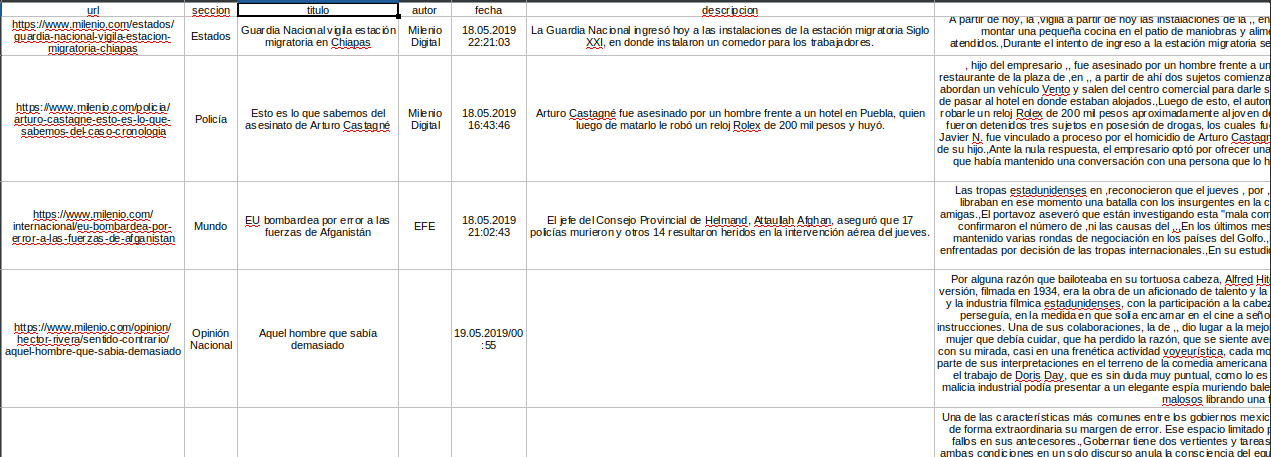
\includegraphics[scale=.3]{imagenes/Capitulo5/9}
  \caption{Resultados obtenidos de la extracción del sitio web almacenado en un archivo CSV.}
  \label{fig:nueve}
\end{figure}

%-----------------------------------------------------------------------------------------%
\subsection{Consideraciones}
\begin{itemize}
  \item Se debe tener conocimiento de XML para poder realizar las etiquetas que extraen información de la cada sitio web
  \item Cuando la noticia consta de un video, no se obtiene ninguna información adicional de la noticia
  \item Se debe tomar en cuenta que las secciones no están homologadas, es decir a pesar de que de la misma página existan varias secciones 
en la cual una noticia puede ser clasificada.
  \item La distribución de la información de una noticia varia dependiendo a la sección y sitio web.
  \item Se acotó el periodo de búsqueda de noticias ya que algunos sitios web muestran las noticias más recientes.
\end{itemize}

%-----------------------------------------------------------------------------------------%
\subsection{Conclusiones}
%Conclusiones
%A pesar de extraer la mayoría de etiquetas requeridas, existen algunos datos que se encuentran en una sola etiqueta.
El 75\% de los sitios web seleccionados contienen las secciones definidas. sin embargo
los sitios web de foros de noticias (Aristegui Noticias, SDP Noticias y Sopitas) tienen muy pocas secciones. A demás 
se logró desarrollar un recolector de noticias que permite extraer el contenido deseado de cada portal como las secciones de los artículos y las URLs que dirigen a noticias asociadas.

%Escribirlo de manera más precisa

%-----------------------------------------------------------------------------------------%
\section{Trabajo a futuro}
\begin{itemize}
  \item Una vez que se obtuvo la extracción de las noticias, analizarán para su integración al corpus
  \item Corregir las reglas para la extracción de la información de los sitios web, y así evitar extraer información con código HTML
  \item Agregar reglas para cada etiqueta, de manera tal manera que se obtenga la información necesaria
  \item Realizar el clasificador de noticias aplicando las técnicas de clasificación previamente definidas
\end{itemize}



  \newpage
   \TChapter{Implementacion y Pruebas}{epsilon}
\ \\\\

\section{Recolección}

%-------------------------------Recolección----------------------------------------------%

El proceso de recolección es parte fundamental del presente trabajo terminal, ya que permitió conformar el corpus necesario para llevar a cabo la etapa de entrenamiento, este proceso se llevo a cabo por etapas.

\begin{itemize}
	\item Seleccionar los sitios web
	\item Información a recolectar
	\item Análisis del sitio web
	\item Proceso de recolección
\end{itemize}

\subsection{Selección de sitios web}

Se han seleccionado los diarios Aristegui Noticias, El Economista, La Jornada, La Prensa, Proceso, Sopitas y TV Azteca para recolectar noticias, fueron seleccionados debido a que forman parte de los sitios web más consultados, sin embargo durante la etapa de recolección se descartaron ciertos sitios debido a que ya no permiten realizar \textit{web scraping}


\subsection{Información recolectada}

Se llevó a cabo un análisis acerca de la información que contiene cada una de las noticias y con base en ello se determinó recolectar la siguiente información:

\begin{itemize}
	\item URL de la noticia
	\item Título
	\item Fecha
	\item Sección
	\item Autor
	\item Descripción
	\item Noticia
\end{itemize}

Cabe destacar que no toda la información recuperada fue utilizada en el proceso de entrenamiento, sin embargo se considerarón los puntos anteriores ya que la mayor parte de las noticias cuentan con esa información.


\subsection{Análisis de sitios web}

Una vez definida la información requerida de cada noticia se realizó un análisis sobre la estructura HTML de cada sitio web, con el fin de realizar expresiones \textit{XPath} que nos permitieran recorrer y procesar un documento XML, dado que cada sitio web cuenta con una estructura diferente, fue necesario realizar el análisis de manera individual, cabe mencionar que existen sitios los cuales realizan actualizaciones a sus páginas por lo cual era necesario realizar el análisis cada dos meses.

Una expresión \textit{XPath} de ruta nos permite buscar y seleccionar los distintos nodos de un documento XML, en el siguiente Cuadro \ref{box:xmlEjemplo} se muestra un ejemplo de un documento XML.

\begin{mygraybox}[label={box:xmlEjemplo}]{Documento XML} 
<nota>\\
	<para>Daniel</para>\\
	<de>Andres</de>\\
	<titulo>Recordatorio</titulo>\\
	<texto>Don't forget me this weekend!</texto>\\
</nota>
\end{mygraybox}

\subsection{Proceso de recolección de noticias}

Existen diversas técnicas y herramientas para la recolección de información, sin embargo en el presente trabajo han sido utilizadas técnicas de \textit{web scraping}.

La siguiente Figura \ref{Fig:recoleccion} muestra el proceso que se lleva a cabo durante la recolección utilizando web scraping.

\begin{figure}[H]
	\centering
	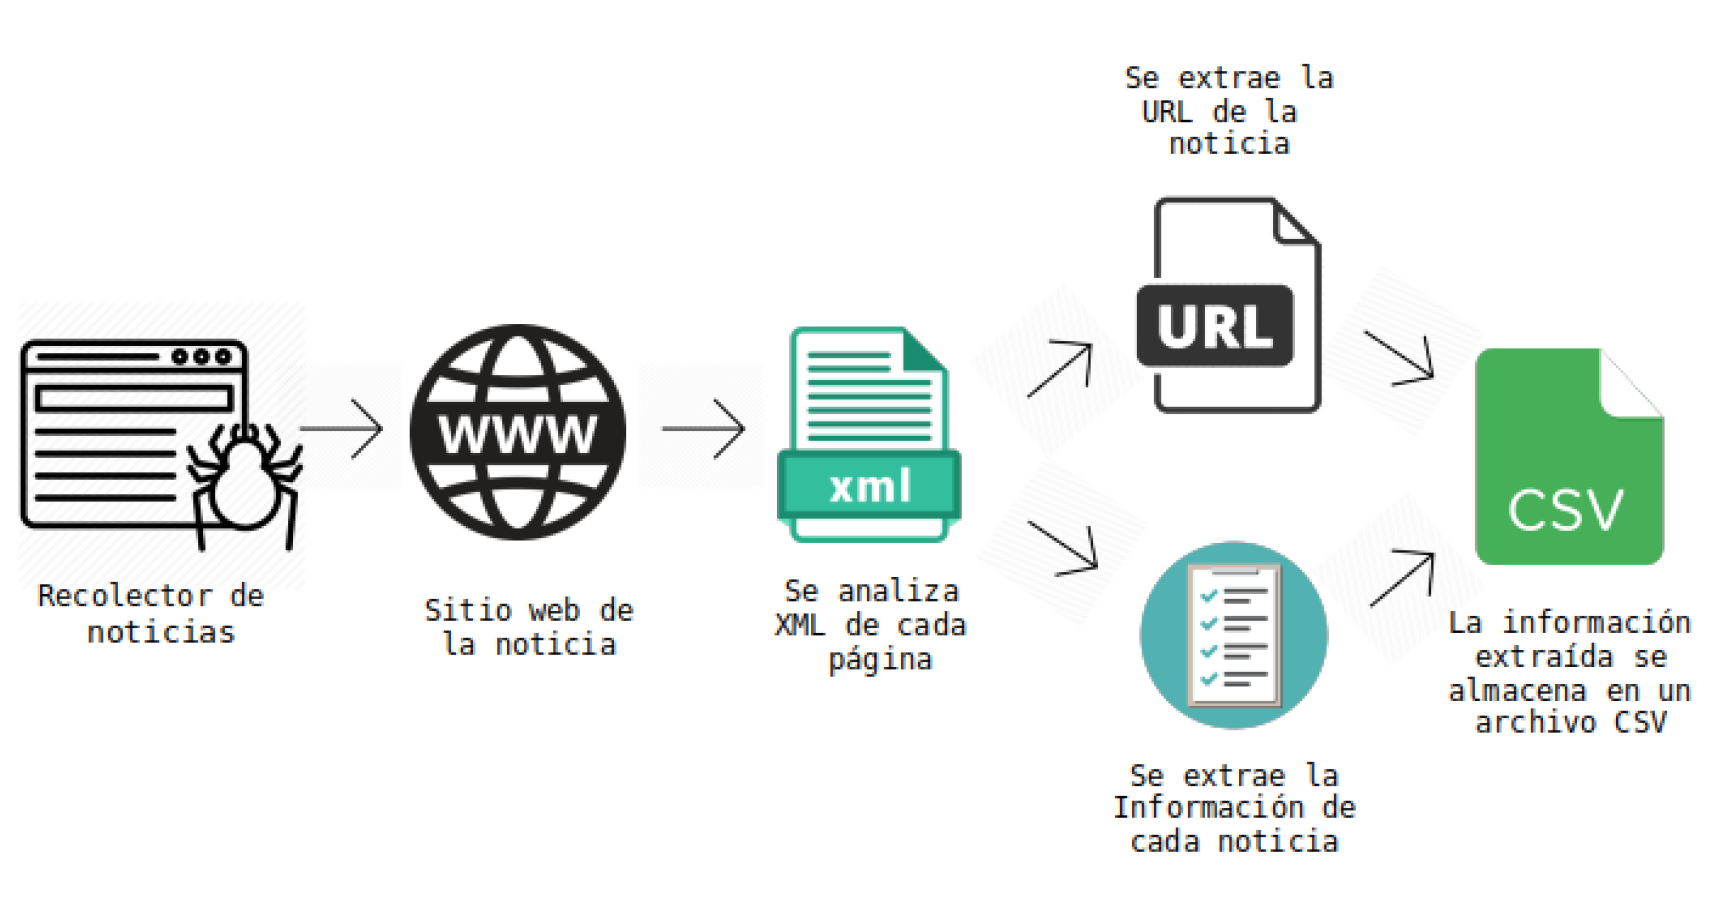
\includegraphics[scale=.2]{imagenes/Capitulo5/recoleccion.png}
	\caption{Proceso de recolección}
	\label{Fig:recoleccion}
\end{figure}

Es necesario contar con noticias de las secciones (Ciencia y Tecnología, Cultura, Deportes, Economía y Política), por lo cual se realizó un crawler por sección, con el fin enriquecer el número de noticias de cada sección, permitiendo obtener mejores resultados en la práctica.
\\
Para generar nuestro corpus, se recolectaron noticias durante el periodo de julio a septiembre con un intervalo de dos días, con el fin de no tener noticias repetidas y evitar ser bloqueados debido alnúmero de peticiones realizadas al sitio web. 
\\
Una vez finalizado el proceso de recolección los resultados obtenidos por sección se muestra en la Figura  \ref{Fig:notseccionV1}.

\begin{figure}[H]
	\centering
	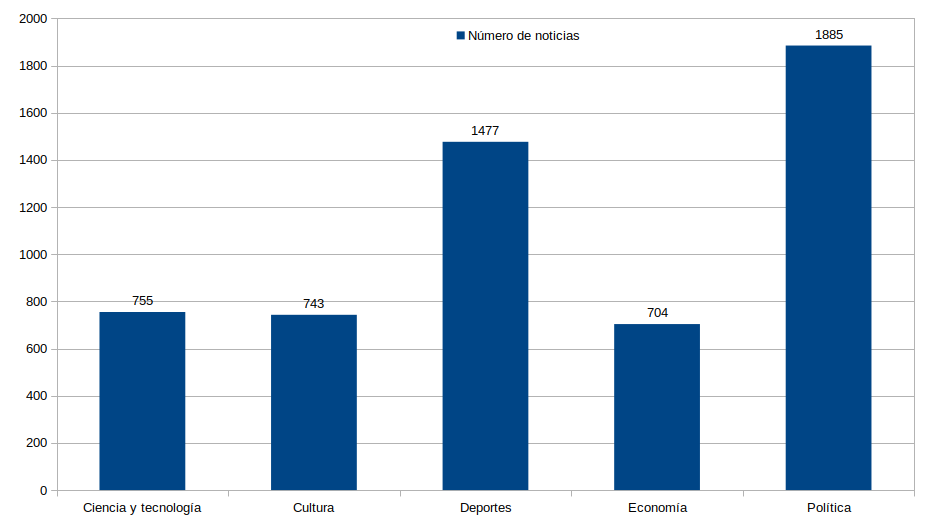
\includegraphics[scale=.6]{imagenes/Capitulo5/noticiasPorSeccionV1.png}
	\caption{Noticias recolectadas durante el primer corte.}
	\label{Fig:notseccionV1}
\end{figure}

Cabe destacar que el número de noticias por sección no se encontraba balanceado debido a que no existía un gran número de sitios que publicarán noticias de cultura, por ello se decidió continuar con el proceso de recolección de noticias, con el fin de balancear el corpus y así nuestros resultados obtenidos en la práctica fueran mejores.
\\
Una vez finalizada la segunda etapa de recolección los nuevos resultados se muestran en la Figura \ref{Fig:notseccion}

\begin{figure}[H]
	\centering
	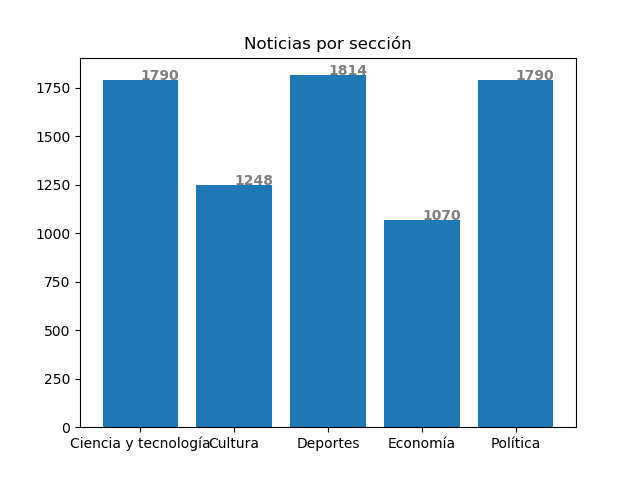
\includegraphics[scale=.6]{imagenes/Capitulo5/noticiasPorSeccion.png}
	\caption{Numero total de noticias recolectadas por sección.}
	\label{Fig:notseccion}
\end{figure}

Las resultados obtenidos por cada sitio web, se muestran en las siguientes Figuras.
\\
\begin{figure}[H]
	\centering
	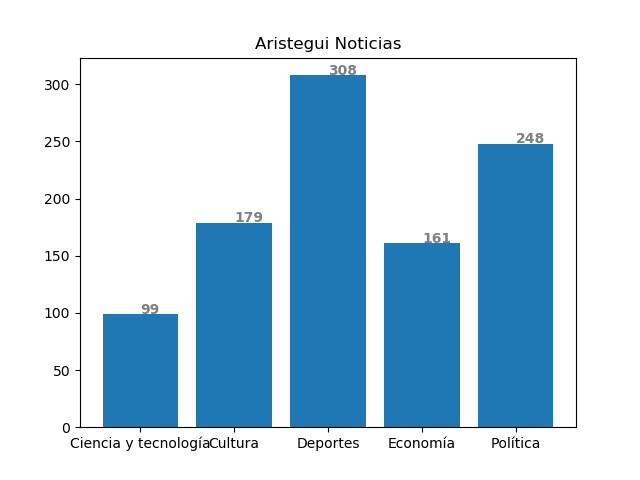
\includegraphics[scale=.45]{imagenes/Capitulo5/aristegui.png}
	\caption{Total de noticias recolectadas del sitio web de Aristegui Noticias}
	\label{Fig:notsitioaristegui}
\end{figure}

\begin{figure}[H]
	\centering
	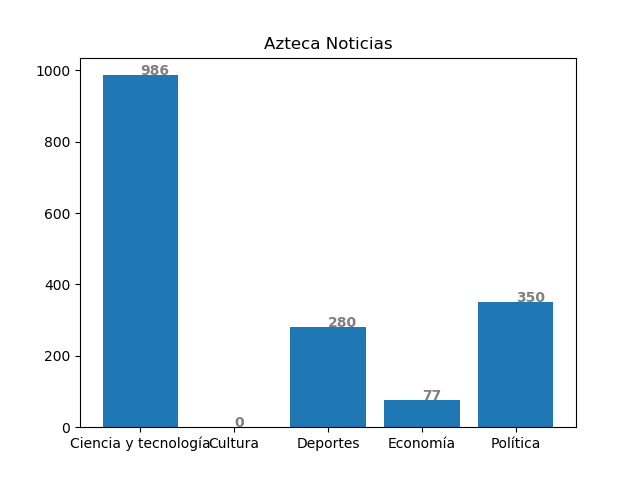
\includegraphics[scale=.45]{imagenes/Capitulo5/azteca.png}
	\caption{Total de noticias recolectadas del sitio web de Azteca Noticias}
	\label{Fig:notsitioazteca}
\end{figure}

\begin{figure}[H]
	\centering
	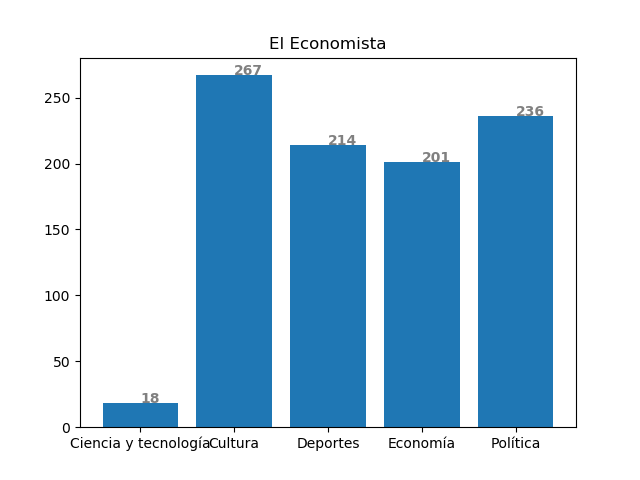
\includegraphics[scale=.45]{imagenes/Capitulo5/economista.png}
	\caption{Total de noticias recolectadas del sitio web de El Economista}
	\label{Fig:notsitioeconomista}
\end{figure}

\begin{figure}[H]
	\centering
	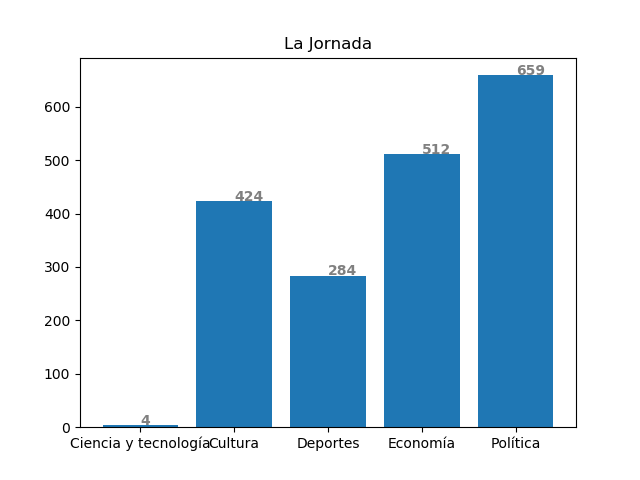
\includegraphics[scale=.45]{imagenes/Capitulo5/jornada.png}
	\caption{Total de noticias recolectadas del sitio web de La Jornada}
	\label{Fig:notsitiojornada}
\end{figure}

\begin{figure}[H]
	\centering
	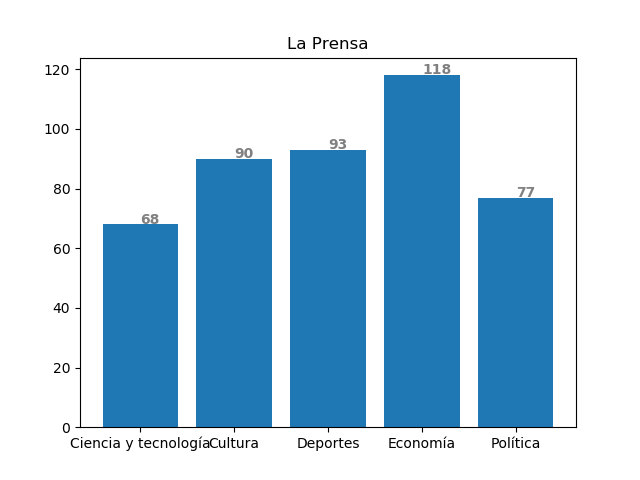
\includegraphics[scale=.45]{imagenes/Capitulo5/prensa.png}
	\caption{Total de noticias recolectadas del sitio web de La Prensa}
	\label{Fig:notsitioprensa}
\end{figure}

\begin{figure}[H]
	\centering
	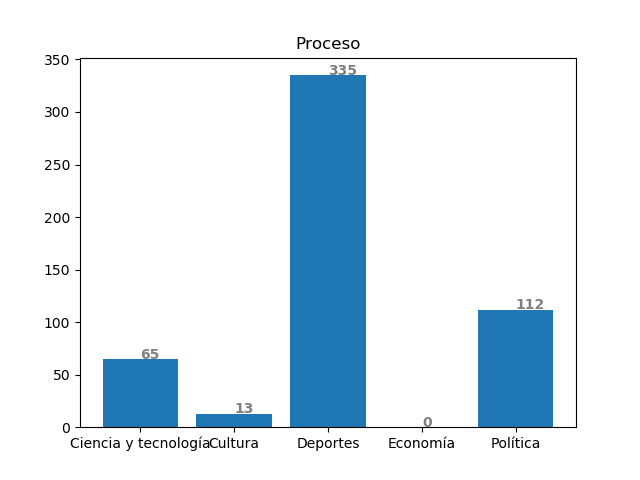
\includegraphics[scale=.45]{imagenes/Capitulo5/proceso.png}
	\caption{Total de noticias recolectadas del sitio web de Proceso}
	\label{Fig:notsitioproceso}
\end{figure}

\begin{figure}[H]
	\centering
	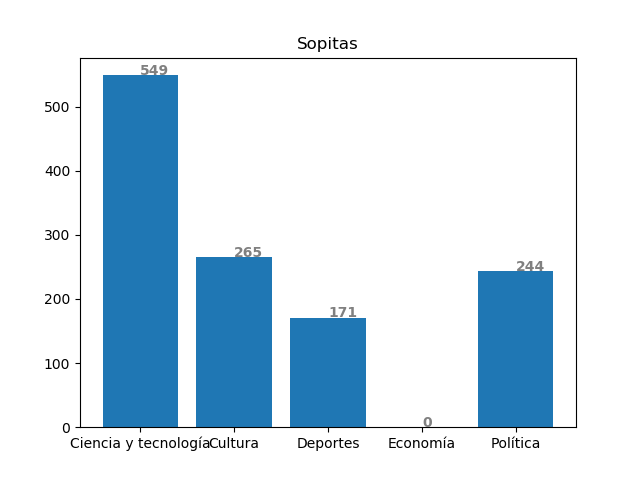
\includegraphics[scale=.45]{imagenes/Capitulo5/sopitas.png}
	\caption{Total de noticias recolectadas del sitio web de Sopitas}
	\label{Fig:notsitiosopitas}
\end{figure}

Una vez concluida la recolección de noticias se procedió con el balanceo de noticias quedando un total de 700 noticias por sección.
\newpage
\section{Entrenamiento de clasificador}
%\HSection{ENTRENAMIENTO}

El segundo pilar del trabajo terminal es entrenar un algoritmo (de aprendizaje automático), para clasificar las noticias en las secciones \textbf{Ciencia y tecnología}, \textbf{Política}, \textbf{Deportes}, \textbf{Economía} y \textbf{Cultura}. Cabe destacar que el clasificador resolverá un problema multiclase (ver \Tref{cp3:multinomial}{Clasificación multiclase}) debido a que la entrada es una artículo y como salida brinda la pertenencia a una sección  de 5 posibilidades. El proceso de entrenamiento se muestra en la Figura \ref{fig:cp5:procesoE}.\\



En este punto es importante mencionar que existe un trabajo terminal previo (TT 2017-A042) el cual ha generado un modelo para clasificar noticias por secciones, sin embargo existen diferencias importantes entre el TT 2017-A042 y el propuesto en este documento, las cuales son mostradas en la Figura \ref{cp5:diferenciastt}.



\begin{figure}[h]
\centering
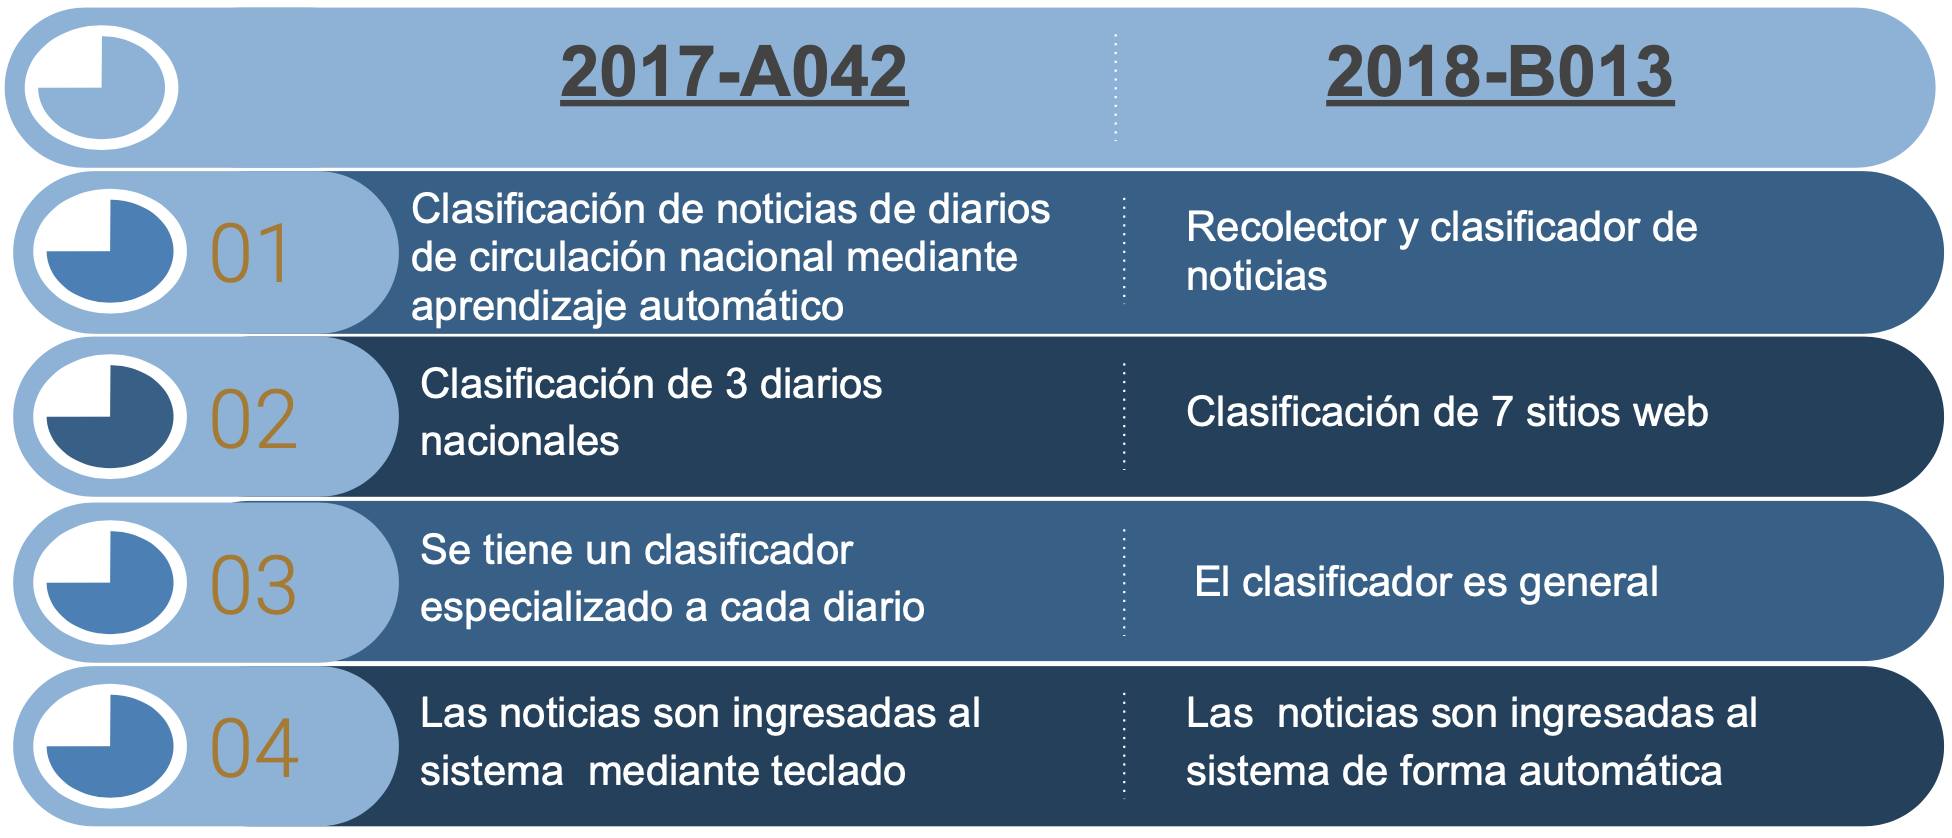
\includegraphics[scale=0.35]{imagenes/capitulo5/entrenamiento/diferenciastt.png}
\caption{Diferencias del clasificador en el TT 2017-A042 y 2018-B013}
\label{cp5:diferenciastt}
\end{figure} 

Como se puede observar en la Figura \ref{cp5:diferenciastt} el modelo del TT 2017-A042 está orientado en la clasificación de noticias de 3 diarios de circulación nacional (\textbf{El Universal}, \textbf{La Jornada} y \textbf{Excélsior}), además de estar enfocado en las secciones particulares de cada periódico y de haber entrenado un algoritmo por cada diario. Por otra parte, este trabajo terminal (TT 2018-B013) tiene como objetivo clasificar noticias en 5 secciones (\textbf{deportes}, \textbf{economía}, \textbf{política}, \textbf{cultura}, \textbf{ciencia y tecnología}), de 7 diferentes sitios web. Es importante mencionar que se entrenará un solo modelo el cual generalice la tarea de clasificación de todas las fuentes noticiosas.\\  

Dada las diferencias se decidió utilizar un nuevo corpus, así como entrenar un nuevo clasificador que se ajuste mejor al objetivo de este trabajo terminal.\\


Como se mencionó en la etapa de recolección, el corpus obtenido contiene 7,707 noticias en total. Sin embargo este contenido debe ser procesado y solo seleccionar los artículos que aporten información para el entrenamiento, al final de la etapa de pre\-procesamiento el corpus será dividió en dos conjuntos: entrenamiento con el 90\% de los artículos y prueba con el 10\%. A continuación se explica la etapa de \textbf{Pre-procesamiento}.\\

\begin{figure}[h]
\centering
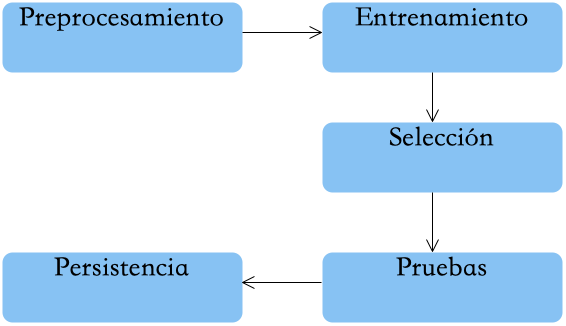
\includegraphics[scale=.55]{imagenes/capitulo5/Entrenamiento/Esquema.png}
\caption{Proceso de entrenamiento}
\label{fig:cp5:procesoE}
\end{figure}



%------------------------------------------------------------------%
\subsection{Preprocesamiento}

Como primera instancia, el corpus creado debe ser procesado, con el fin de crear vectores que representan el contenido de cada artículo de forma ordenada (ver \Tref{cp3:representaciont}{Representación del texto}), de esta manera los algoritmos de clasificación son capaces de entender la información. En cuanto a los datos que son procesados de la noticia cabe mencionar que solo se usa el título y la redacción del artículo, los demás datos (como url, fecha, sección) no son necesarios para el entrenamiento. Este proceso consta de 6 etapas, las cuales son mostradas en la Figura \ref{fig:cp5:preprocesamiento}. \\

Cabe destacar que estas etapas están desarrolladas en un script escrito en el lenguaje \textbf{python 3}, en cada sección se hará mención de las bibliotecas ocupadas.\\

\begin{figure}[h]
\centering
\includegraphics[scale=.55]{imagenes/capitulo5/Entrenamiento/preprocesamiento.png}
\caption{Etapas de preprocesamiento}
\label{fig:cp5:preprocesamiento}
\end{figure}

%----------------------------------%
%\begin{large}
\Tlabel{cp5:limpieza}
\subsubsection{Limpieza}
%\end{large}

Esta etapa consiste en eliminar texto que no brinda información útil para el entrenamiento como, hipertexto (ver \Tref{cp3:html}{HTML}), símbolos especiales (como \# $\dagger$ $\sqrt{ }$), \textit{emojis} (como \dSmiley \dCooley \dNinja). Por ejemplo el texto \ref{box:cp5:texto} muestra la redacción de una noticia con la información descargada de una pagina web. El resultado de limpiar la noticia se muestra en el texto \ref{box:cp5:limpio}. Se puede observar que se han eliminado los elementos $<p>\ </p>\ <!--\ -->$ \# $\dagger$ \dSmiley \dCooley \dInnocey.\\

Para realizar esta tarea se han utilizado las bibliotecas: \textbf{pandas} como medio de lectura de archivos tipo \textbf{CSV} (\textit{comma separeted values}, por sus siglas en ingles); \textbf{re} la cual permite evaluar expresiones regulares con el objetivo de eliminar símbolos; \textbf{demoji} quien permite eliminar \textit{emojis} dentro del texto.\\

\begin{mygraybox}[label={box:cp5:texto}]{Texto de entrada} 
$<p>\dagger$$\ \ \ $ El número 343 de El Trimestre Económico,$\otimes$ revista emblemática del Fondo de Cultura 
$<!--\ -->$
Económica (FCE), será * * * presentado por David Ibarra Muñoz \dSmiley , Carlos Tello Macías \dCooley , Alicia Puyana \dInnocey y Pablo Ruiz Nápoles el martes 27 de agosto a las 6 de la tarde, en la librería Rosario Castellanos, ubicada en avenida Tamaulipas \# 202, en la colonia Condesa de la capital mexicana.$</p>$
\end{mygraybox}

\ \\

\begin{mygraybox}[label={box:cp5:limpio}]{Texto limpio} 
El número 343 de El Trimestre Económico, revista emblemática del Fondo de Cultura 
Económica (FCE), será presentado por David Ibarra Muñoz, Carlos Tello Macías , Alicia Puyana y Pablo Ruiz Nápoles el martes 27 de agosto a las 6 de la tarde, en la librería Rosario Castellanos, ubicada en avenida Tamaulipas 202, en la colonia Condesa de la capital mexicana.
\end{mygraybox}
%----------------------------------%
%\begin{large}
\subsubsection{Filtro de longitud}
%\end{large}

Con base en la regla de negocio \RNref{RN1}{Número de palabras} se ha definido 180 palabras como longitud mínima de las noticias, incluyendo en la definición de palabra números, signos de puntuación y exclamación.
Para esto después de haber concluido el proceso de limpieza se pregunta por la longitud de la cadena (sin contar los espacios) y si esta es mayor o igual a 180, entonces es un artículo válido para utilizar en el entrenamiento de lo contrario no es tomado en cuenta.\\


%----------------------------------%
%\begin{large}
\subsubsection{Delimitación del corpus}
%\end{large}

En este punto del proceso, la cantidad de artículos ha disminuido (como se observa en la Figura \ref{fig:cp5:noticiasSecciones}), sin embargo la distribución por sección no es homogénea, esta situación crea un sesgo en el corpus y después en la etapa de \textbf{Entrenamiento} los algoritmos pueden desarrollar una preferencia por la categoría con mas datos. Por está razón se debe acotar la cantidad de noticias.\\

Como se muestra en la Figura \ref{fig:cp5:noticiasSecciones} cada sección contiene al menos 700 noticias, por lo tanto este es el número definido para delimitar el número de artículos. De esta manera el corpus se ha definido como se muestra en la Figura \ref{fig:notBalanceadas}, obteniendo un total de 3,500 noticias.\\

\begin{figure}[H]
	\centering
	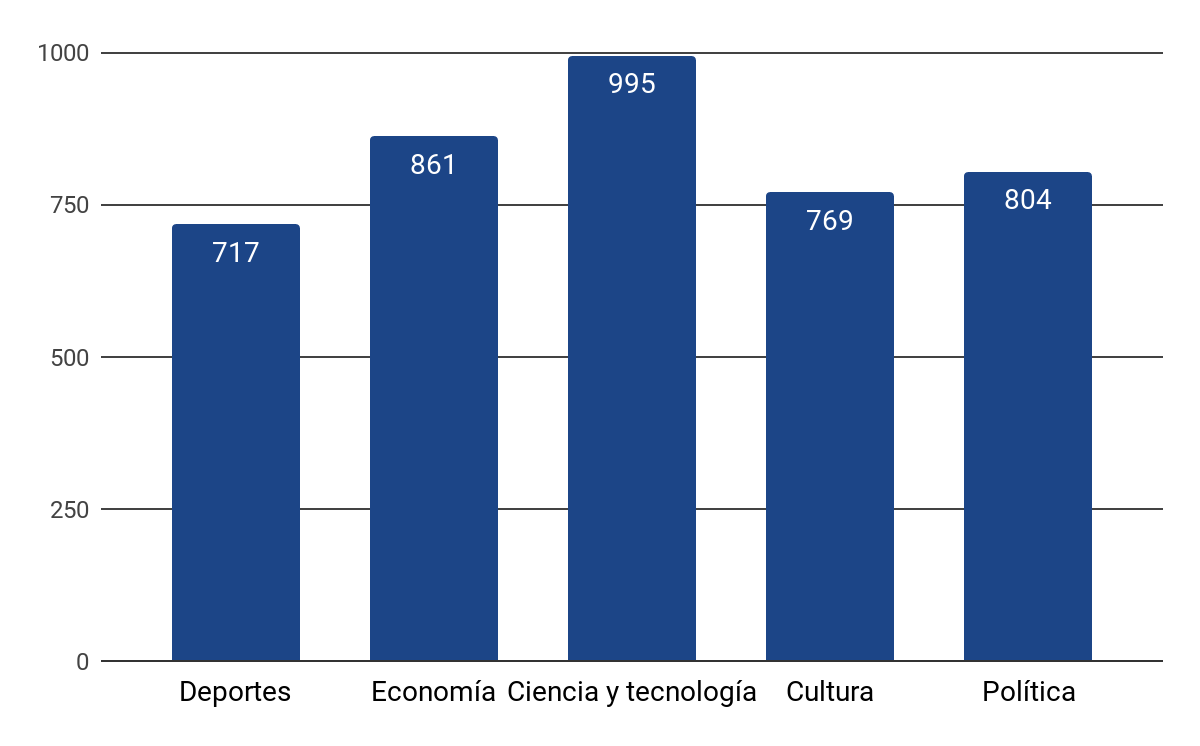
\includegraphics[scale=.33]{imagenes/Capitulo5/Entrenamiento/noticiasSecciones.png}
	\caption{Noticias por sección}
	\label{fig:cp5:noticiasSecciones}
\end{figure}


\begin{figure}[H]
	\centering
	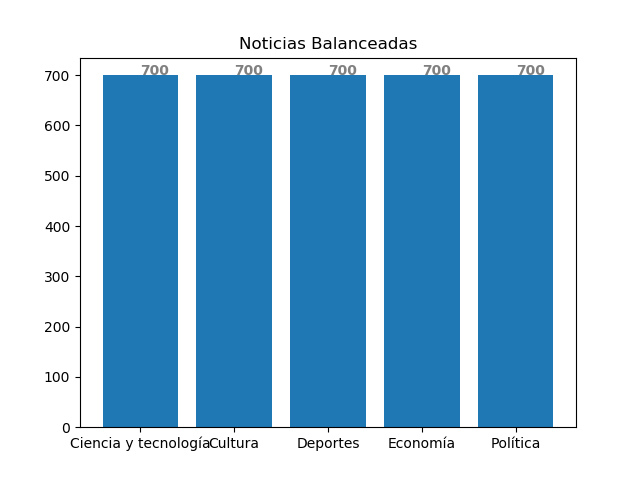
\includegraphics[scale=.5]{imagenes/Capitulo5/noticiasBalanceadas.png}
	\caption{Noticias por sección}
	\label{fig:notBalanceadas}
\end{figure}

%----------------------------------%
%\begin{large}
\subsubsection{Tokenizar}
%\end{large}
\Tlabel{cp5:tokenizacion}
La etapa de tokenización consiste en separar el texto en sus elementos mínimos llamados tokens, donde se separan palabras, signos de puntuación, llaves y números mediante un espacio. Continuando con el ejemplo \ref{box:cp5:limpio} donde el texto se encuentra limpio, se procede a su tokenización. El resultado es mostrado en el Cuadro \ref{box:cp5:tokenizar}. Para remarcar el ejemplo observe la palabra entre paréntesis \textbf{(FCE)} la cual es separada en \textbf{( FCE )} mostrando que ahora cada elemento representa un token individual. Para el desarrollo de esta tarea se utilizó la biblioteca \textbf{RegexpTokenizer}.\\

\begin{mygraybox}[label={box:cp5:tokenizar}]{Texto tokenizado} 
El número 343 de El Trimestre Económico , revista emblemática del Fondo de Cultura 
Económica ( FCE ) , será presentado por David Ibarra Muñoz , Carlos Tello Macías , Alicia Puyana y Pablo Ruiz Nápoles el martes 27 de agosto a las 6 de la tarde , en la librería Rosario Castellanos , ubicada en avenida Tamaulipas 202 , en la colonia Condesa de la capital mexicana .
\end{mygraybox}

%----------------------------------%
%\begin{large}
\subsubsection{Lematizar}
%\end{large}
\Tlabel{cp5:lematizacion}
Lematizar es el proceso de reducir cada palabra a su lema, con el fin de disminuir la dispersión en el texto, por ejemplo las palabras correrás, corriendo, corrí, tienen como lema el verbo correr, el plural niños tiene como lema niño (ver \Tref{cp3:lematizacion}{Lematización}). Para realizar esta tarea se ha usado \textbf{spacy} el cual es una librería de código abierto, con el diccionario \textit{es\_core\_news\_sm} quien permite analizar el léxico del lenguaje español.\\

Siguiendo con las etapas del proceso se toma el texto \ref{box:cp5:tokenizar} como entrada al programa y este da como salida el texto que se muestra en el Cuadro \ref{box:cp5:lematizado}.\\

\begin{mygraybox}[label={box:cp5:lematizado}]{Texto lematizado} 
el número 343 de el trimestre económico , revista emblemático del fondo de cultura económica ( fce ) , ser presentar por david ibarra muñoz , carlos tello macías , alicia puyana y pablo ruiz nápoles el martes 27 de agostar a los 6 de lo tardar , en lo librería rosario castellanos , ubicar en avenir tamaulipas 202 , en lo colonia condesa de lo capital mexicano .
\end{mygraybox}
\ \\

Cuando el proceso de lematización concluye se genera un identificador único para cada noticia el cual se define de la siguiente forma 

\begin{equation*}
id=<Identificador\ de\ sitio\ web><Numero\ de\ noticias>
\end{equation*}
 
donde \textbf{Identificador de sitio web} define un número único para hacer referencia a los sitios web (ver Tabla \ref{tab:cp5:sitioweb}) y  \textbf{Número de noticias} es el número del artículo.

\begin{table}[h]
\centering
	\begin{tabular}{|l|l|}
	%-----------------------Ecanbezado-----------------------------------%
		\hline
		\multicolumn{1}{| >{\columncolor{white!30!black}}l|}{ \textcolor{myWhite}{\textbf{Número}} }&
		\multicolumn{1}{| >{\columncolor{white!30!black}}l|}{ \textcolor{myWhite}{\textbf{Página web}} }\\
		\hline
	%------------------------------------------------%

		\textbf{100} & Aristegui noticias\\
		\hline
		\textbf{200} & Tv azteca\\
		\hline

		\textbf{300} & El economista\\
		\hline

		\textbf{400} & La jornada\\	
		\hline

		\textbf{500} & La prensa\\
		\hline

		\textbf{600} & Proceso\\
		\hline

		\textbf{700} & Sopitas\\
		\hline

	\end{tabular}\\
\caption{Identificador de sito web}
\label{tab:cp5:sitioweb}
\end{table}


Como segundo paso las noticias son almacenadas en un archivo con extensión \textbf{TXT}, los elementos por almacenar son \textbf{id}, \textbf{titulo}, \textbf{noticia} y \textbf{sección}, los cuales son separados por los caracteres \&\&\&\&\&. El Cuadro \ref{box:cp5:archivo} muestra un ejemplo de la estructura del archivo.\\

\begin{mygraybox}[label={box:cp5:archivo}]{Estructura de archivo} 
\textbf{id}\&\&\&\&\&\textbf{titulo}\&\&\&\&\&\textbf{noticia}\&\&\&\&\&\textbf{seccion}\\
1001\&\&\&\&\&Titulo 1\&\&\&\&\&Contenido noticia 1\&\&\&\&\&0\\
...\\
5003500\&\&\&\&\&Titulo 3500\&\&\&\&\&Contenido noticia 3500\&\&\&\&\&4
\end{mygraybox}

%----------------------------------%

%\begin{large}
\Tlabel{cp5:divisionC}
\subsubsection{División del corpus}
%\end{large}


Para el correcto diseño y evaluación del algoritmo clasificador se requiere dividir el corpus en dos conjuntos: \textbf{entrenamiento} y \textbf{prueba}, con un 90\% y 10\% del total del corpus respectivamente. En cada grupo deben estar repartidas noticias de las 5 secciones definidas, sin embargo los artículos almacenados están ordenados de forma descendente como: \textbf{Deportes}, \textbf{Economía}, \textbf{Política}, \textbf{Cultura}, \textbf{Ciencia y tecnología}, para seleccionar de forma distribuida los datos se ha utilizado una técnica llamada \textit{Shuffle}.\\

\textit{Shuffle} consiste en brindar un arreglo con los identificadores de las noticias y un número (nombrado usualmente como semilla), quien generar un nuevo orden en los identificadores de acuerdo a los números pseudo aleatorios que retorna esta función, tomando este como el nueva orden de los textos en el archivo de almacenamiento. Para el desarrollo de esta etapa se ha utilizado la biblioteca \textbf{Shuffle} con una semilla de 5.\\

Para ilustrar un ejemplo, en el cuadro \ref{box:cp5:ids} se muestra un conjunto de identificadores ordenados por el último número del $id$, al utilizar la función \textit{Shuffle} con una semilla de 2, se genera un nuevo orden el cual es mostrado en el Cuadro \ref{box:cp5:shuffle}.\\


\begin{mygraybox}[label={box:cp5:ids}]{Identificadores de noticias} 
\begin{equation*}
\begin{bmatrix}
1001 & 2002 & 3003 & 4004 & 5005 & 6006 & 7007 & 1008\\ 
\end{bmatrix}
\end{equation*}
\end{mygraybox}


\begin{mygraybox}[label={box:cp5:shuffle}]{Nuevo orden de ID's} 
\begin{equation*}
\begin{bmatrix}
5005 & 2002 & 7007 & 3003 & 4004 & 1008 & 6006 & 1001\\
\end{bmatrix}
\end{equation*}
\end{mygraybox}

La distribución generada por esta función es almacenada en un archivo, y como último paso se han tomado las primeras 350 noticias de forma manual y se han colocado en un archivo diferente, definido así las noticias de entrenamiento (con 3,150) y de prueba (con 350).\\

La cantidad de noticias por sección del conjunto de entrenamiento se muestran en la Figura \ref{fig:cp5:seccionE} y del conjunto de prueba en la Figura \ref{fig:cp5:seccionP}.



\begin{figure}[H]
\centering
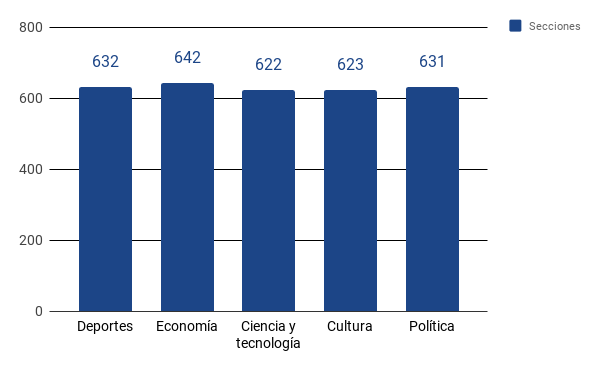
\includegraphics[scale=.67]{imagenes/capitulo5/Entrenamiento/SeccionesE.png}
\caption{Corpus de entrenamiento}
\label{fig:cp5:seccionE}
\end{figure}

\begin{figure}[H]
\centering
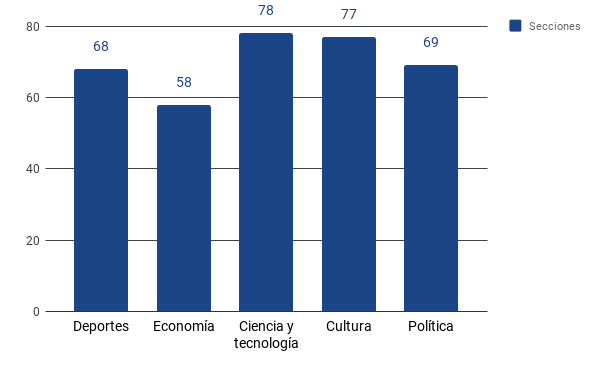
\includegraphics[scale=.67]{imagenes/capitulo5/Entrenamiento/SeccionesP.png}
\caption{Corpus de prueba}
\label{fig:cp5:seccionP}
\end{figure}

%\begin{figure}[h]
%\centering
%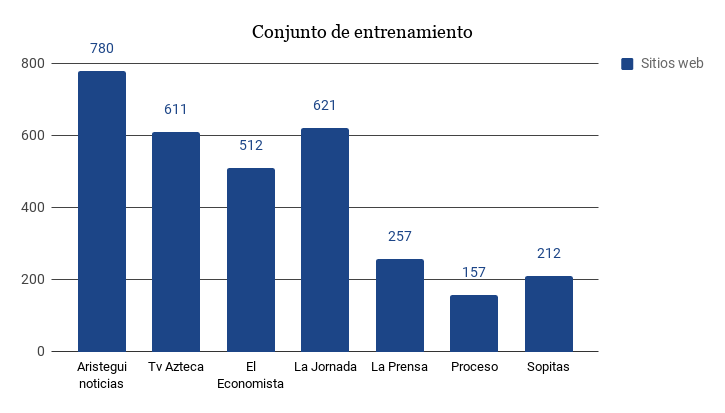
\includegraphics[scale=.6]{imagenes/capitulo5/Entrenamiento/SitiosE.png}
%\caption{Número de noticias pertenecientes a los sitios web}
%\label{fig:cp5:sitiosE}
%\end{figure}



%------------------------------------------------------------------%
\subsection{Entrenamiento}

Para crear un modelo clasificador usando aprendizaje supervisado (ver \Tref{cp3:asupervisado}{Aprendizaje supervisado}), se debe construir dos conjuntos etiquetados: entrenamiento para el proceso de aprendizaje y otro de prueba, para medir su precisión. En la sección anterior estos grupos se han formado con noticias de 5 secciones: \textbf{Deportes}, \textbf{Economía}, \textbf{Política}, \textbf{Cultura}, \textbf{Ciencia y tecnología}. Ambos conjuntos de datos serán usados por 4 algoritmos (seleccionados con base en el estado del arte ver \Tref{cp2:estadodelarte}{Estado del arte}), los cuales son:

\begin{itemize}
	\item \textbf{Naive Bayes} (ver \Tref{cp3:naive}{Naive Bayes})
	\item \textbf{Regresión logística} (ver \Tref{cp3:regresion}{Regresión logística})
	\item \textbf{Máquina de soporte vectorial} (ver \Tref{cp3:msv}{MSV})
	\item \textbf{Random Forest} (ver \Tref{cp3:random}{Random Forest})
\end{itemize}

El proceso de entrenamiento consta de 5 pasos los cuales se muestran en la Figura \ref{fig:cp5:entrenamiento}.

\begin{figure}[h]
\centering
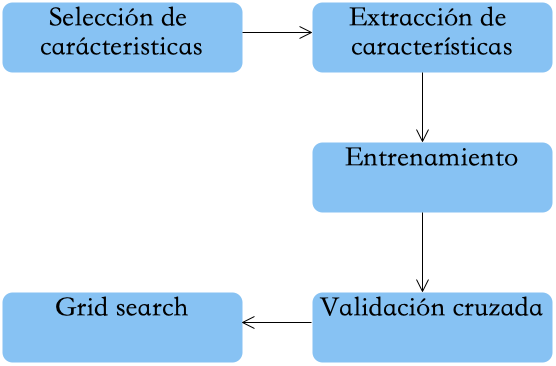
\includegraphics[scale=.55]{imagenes/capitulo5/Entrenamiento/Entrenamiento.png}
\caption{Etapas de entrenamiento}
\label{fig:cp5:entrenamiento}
\end{figure}

El desarrollo se ha implementado en el lenguaje de programación \textbf{Python 3}, utilizando la biblioteca \textbf{scikit learn} quien permite crear instancias de los algoritmos mencionados.\\

Como primer paso del entrenamiento, el corpus debe ser representado mediante conjuntos de vectores numéricos, esta es llamada representación vectorial (ver \Tref{cp3:representaciont}{Representación del texto}). Para lograr este objetivo, del corpus se deben seleccionar características que definan los elementos del vector numérico.\\

%----------------------------------%
%\begin{large}
\Tlabel{cp5:extraccion}
\subsubsection{Extracción de características}
%\end{large}

La extracción de características cuenta con dos tareas importantes: extraer el vocabulario y crear un vector de características.\\

Cada clase de noticias contiene un conjunto de palabras que son comunes en su ámbito, al analizar el léxico usado se observa los tecnicismos usados, por ejemplo en la sección deportes se ocupa, fútbol, jugador, ganador; en política, presidente, corrupción, PRI; en ciencia y tecnología, investigación, descubrimiento, publicación y así sucesivamente, por lo tanto estos vocablos pueden ser definidos como características que identifican a una sección. En este sentido la extracción de características es el proceso de tomar las palabras de las noticias para formar un vocabulario.\\

Para ejemplificar esta tarea observe el Cuadro \ref{box:cp5:corpus} el cual es un corpus de 4 oraciones. Una vez realizado el proceso de extracción de características se obtiene el vocabulario el cual el mostrado en el Cuadro \ref{box:cp5:caracteristicas}.\\

\begin{mygraybox}[label={box:cp5:corpus}]{Corpus} 
\begin{equation*}
\begin{bmatrix}
Este&es&la&primera&noticia&noticia\\
Esta&noticia&es&la&segunda&noticia&???\\
Y&este&es&la&tercera\\
Es&este&la&primera&noticia&????\\
\end{bmatrix}
\end{equation*}
\end{mygraybox}
\ \\
\begin{mygraybox}[label={box:cp5:caracteristicas}]{Selección de características} 
\begin{equation*}
\begin{bmatrix}
es & esta & este & la & noticia & primera & segunda & tercera & y & ?
\end{bmatrix}
\end{equation*}
\end{mygraybox}

%----------------------------------%



Después de extraer el  vocabulario, se crea un espacio vectorial por cada noticia donde cada elemento del vector representa la presencia o ausencia de una característica (palabra). Cabe mencionar que las características son extraídas de 2 formas, binario (donde 1 representa la presencia de la característica y 0 la ausencia ) y por frecuencia (donde se cuenta el número de veces que cada característica aparece). Continuando con el ejemplo del Cuadro \ref{box:cp5:corpus} se extraen las características por frecuencia y el resultado se muestra en el Cuadro \ref{box:cp5:frecuencia}, mientras que el Cuadro \ref{box:cp5:binario} muestra las características extraídas de forma binaria.\\

Para el desarrollo de esta etapa se ha utilizado la biblioteca \textbf{CountVectorizer} quien permite generar la selección y extracción de características, ademas esta es la representación vectorial (de cada noticia) que los algoritmos de clasificación pueden entender y por ende ser entrenados. Cabe destacar que la representación vectorial usada en este trabajo ha sido de forma binaria.\\

\begin{mygraybox}[label={box:cp5:frecuencia}]{Representación por frecuencia} 
\begin{equation*}
\begin{bmatrix}
1 & 0 & 1 & 1 & 2 & 1 & 0 & 0 & 0 & 0\\
1 & 1 & 0 & 1 & 2 & 0 & 1 & 0 & 0 & 3\\
1 & 0 & 1 & 1 & 1 & 0 & 0 & 1 & 1 & 0\\
1 & 0 & 1 & 1 & 1 & 1 & 0 & 0 & 0 & 4\\
\end{bmatrix}
\end{equation*}
\end{mygraybox}

\ \\

\begin{mygraybox}[label={box:cp5:binario}]{Representación binaría} 
\begin{equation*}
\begin{bmatrix}
1 & 0 & 1 & 1 & 1 & 1 & 0 & 0 & 0 & 0\\
1 & 1 & 0 & 1 & 1 & 0 & 1 & 0 & 0 & 1\\
1 & 0 & 1 & 1 & 1 & 0 & 0 & 1 & 1 & 0\\
1 & 0 & 1 & 1 & 1 & 1 & 0 & 0 & 0 & 1\\
\end{bmatrix}
\end{equation*}
\end{mygraybox}

\ \\
%----------------------------------%

%\begin{large}
\subsubsection{Entrenamiento}
%\end{large}


El corpus contiene noticias de varias fuentes, en  las cuales la redacción, coherencia, semántica varía, incluso en la edición de una misma noticia, por lo tanto en el entrenamiento se busca generalizar la clasificación de los artículos, analizando el texto como un conjunto de palabras, sin tomar en cuenta la semántica, esta técnica es llamada bolsa de palabras (ver \Tref{cp3:bolsap}{Bolsa de palabras}).\\

En este punto del trabajo las noticias están representadas en un espacio vectorial, y serán usadas en el proceso de entrenamiento de los algoritmos: \textbf{Naive Bayes}, \textbf{Regresión logística}, \textbf{Máquina de soporte vectorial}, \textbf{Random Forest}. Cada clasificador recibe como entrada un conjunto de vectores etiquetados y como salida se genera un modelo el cual predice la sección de nuevas noticias.\\ 

Para este trabajo se han definido las etiquetas como se muestra en la Tabla \ref{tab:cp5:etiquetas}, esta correspondencia es de secciones de noticias a un número único.\\


\begin{table}[h]
\centering
	\begin{tabular}{|l|l|}
	%-----------------------Ecanbezado-----------------------------------%
		\hline
		\multicolumn{1}{| >{\columncolor{white!30!black}}l|}{ \textcolor{myWhite}{\textbf{Sección}} }&
		\multicolumn{1}{| >{\columncolor{white!30!black}}l|}{ \textcolor{myWhite}{\textbf{Etiqueta}} }\\
		\hline
	%------------------------------------------------%

		\textbf{Deportes} & 0 \\
		\hline

		\textbf{Economía} & 1 \\
		\hline
		\textbf{Política} & 2 \\
		\hline

		\textbf{Cultura} & 3 \\
		\hline

		\textbf{Ciencia y tecnología} & 4 \\	
		\hline

	\end{tabular}\\
\caption{Etiquetas de secciones}
\label{tab:cp5:etiquetas}
\end{table}


El desarrollo ha utilizado una instancia de cada algoritmo, para esto se incluye la biblioteca correspondiente de \textbf{sciktlearn}, las cuales se muestran en la Tabla \ref{tab:cp5:librerias}, la entrada al clasificador es el conjunto de características y las etiquetas correspondientes, esto regresa como resultado un modelo que es capaz de predecir la sección de noticias, sin que estas estén etiquetadas.

\begin{table}[h]
\centering
	\begin{tabular}{|l|l|}
	%-----------------------Ecanbezado-----------------------------------%
		\hline
		\multicolumn{1}{| >{\columncolor{white!30!black}}l|}{ \textcolor{myWhite}{\textbf{Sección}} }&
		\multicolumn{1}{| >{\columncolor{white!30!black}}l|}{ \textcolor{myWhite}{\textbf{Etiqueta}} }\\
		\hline
	%------------------------------------------------%

		\textbf{Naive Bayes} & MultinomialNB \\
		\hline

		\textbf{Máquina de soporte vectorial} & SVC\\
		\hline

		\textbf{Regresión logísitica} &LogisticRegression\\
		\hline

		\textbf{Random Forest} &  RandomForestClassifier\\
		\hline

	\end{tabular}\\
\caption{Biblioteca de algoritmo}
\label{tab:cp5:librerias}
\end{table}




%----------------------------------%

%\begin{large}
\subsubsection{Validación cruzada}
%\end{large}

En el proceso de entrenamiento, los clasificadores reciben un conjunto noticias para ser entrenados y otro para realizar pruebas, sin embargo la selección de los artículos puede ser manipulada para obtener un resultado a conveniencia, siendo esto una mala práctica, por esta razón y en con el objetivo de obtener resultados mas robustos se ha implementado un técnica llamada Validación cruzada (ver \Tref{cp3:validacionc}{Validación cruzada}).\\

Este método consiste en tres pasos: el primero es dividir el corpus en entrenamiento y prueba (este conjunto es llamado pliegue); después se calcula la exactitud de la prueba y es almacenado; como último etapa los dos primeros paso son repetidos $n$ veces y para terminar  se calcula el promedio de la exactitud. En términos generales este promedio nos brinda mayor confianza en el resultado del entrenamiento de cada clasificador.\\

%----------------------------------%

%\begin{large}
\subsubsection{Ajuste de parámetros}
%\end{large}

Como se ha visto, los resultados de la clasificación son medidos por la cantidad de noticias correctas clasificadas, no obstante estos resultados pueden incrementar o decrementar con base a los parámetros ingresados a cada algoritmo.\\

Esta etapa consiste en observar el mejor resultado en la clasificación con los diferentes algoritmos, variando los parámetros y aplicar validación cruzada para medir la precisión. Para ejemplificar este tarea la Figura \ref{fig:cp5:gridbayes} muestra la variación del parámetro \textbf{alpha} en el algoritmo \textbf{Naive bayes} (este parámetro será explicado mas adelante) tomando los valores: 0.5, 1.0, 1.5 y 2.0, aplicando 2 pliegues en la validación cruzada.\\

\begin{figure}[h]
\centering
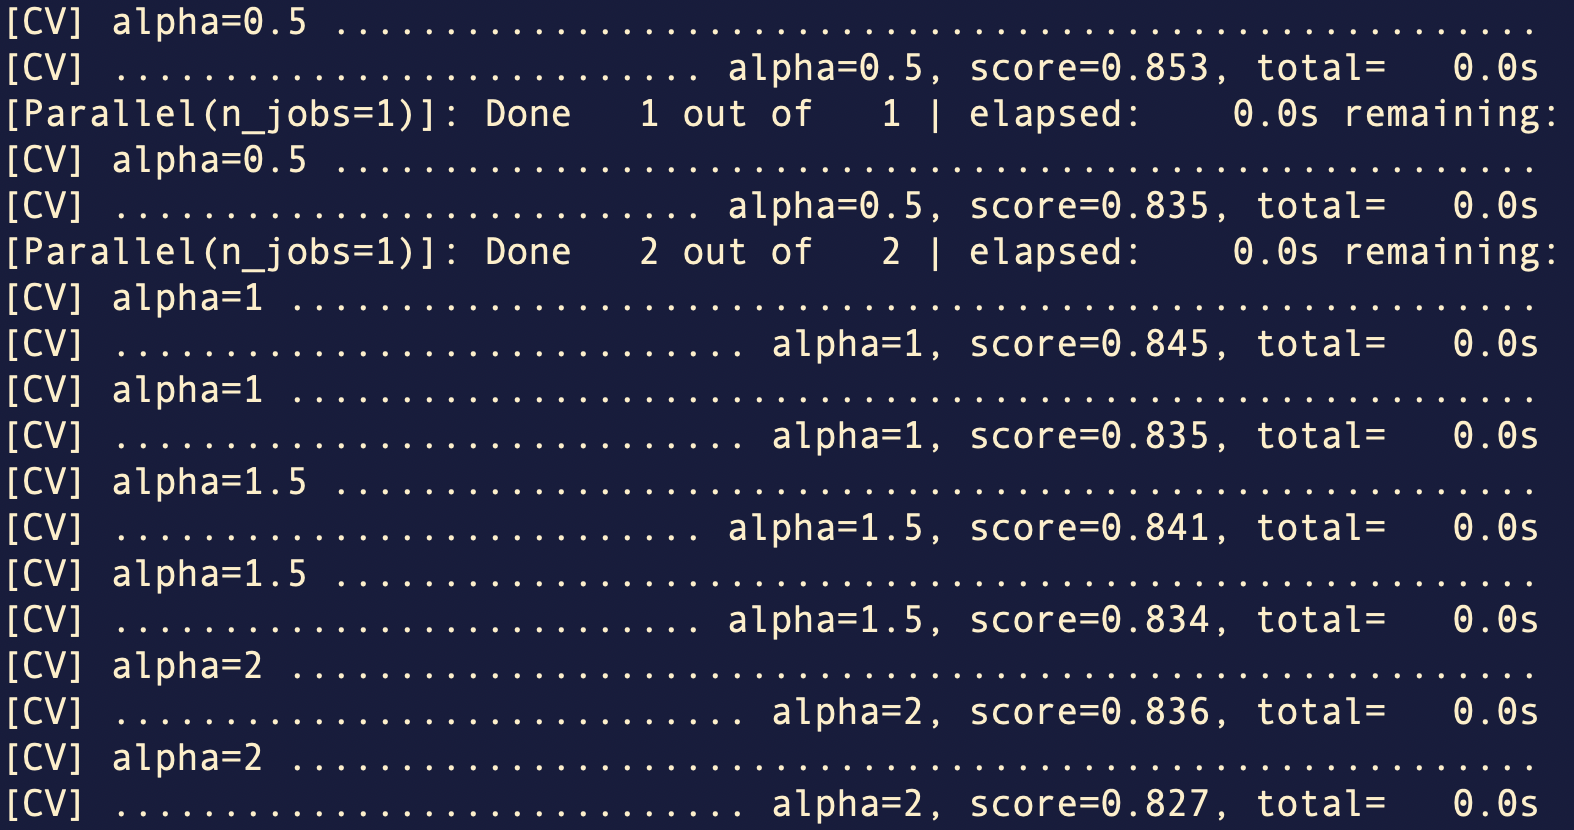
\includegraphics[scale=.5]{imagenes/capitulo5/Entrenamiento/gridbayes.png}
\caption{Corpus de entrenamiento}
\label{fig:cp5:gridbayes}
\end{figure}

Se observa que por cada parámetro implementado en la validación cruzada se muestra el resultado \textbf{score}, el cual es el promedio de la precisión de dicha prueba, se puede observar que el mejor resultado ha sido hecha con el $\alpha=0.5$, con un 85\% de precisión.\\


A continuación se explican los parámetros de cada clasificador: \\

%----------------%
%\begin{Text}
\textbf{Naive Bayes}\\
%\end{Text}
 
El parámetro en el cual se varía en este algoritmo, es un escalar llamado \textbf{Alpha} ($\alpha$). Este es un valor numérico asignado a cada palabra en el corpus con respecto a la frecuencia de aparición en un clase. El valor $\alpha$ evita que la importancia de una palabra se haga cero, \textbf{Alpha} es variado en los valores [$0.5, 1.0, 1.5, 2$].\\


%----------------%
%\begin{Text}
\textbf{Regresión logística}\\
%\end{Text}

%Referencia: https://www.kaggle.com/joparga3/2-tuning-parameters-for-logistic-regression
 Este algoritmo está basado en una regresión lineal y el calculo de probabilidades como se explica en el capitulo 3 (ver \Tref{cp3:regresion}{Regresión logística}). Existen 2  parámetros importantes en este clasificador, optimizando la función $l_1$  y minimizando el costo de la función $l_2$, en el cual existe un escalar $C$, donde: para valores pequeños de este número, los valores de los pesos $w$ (la importancia de cada palabra) se decrementa, teniendo así un modelo muy simple (se pierde información), de lo contrario para valores grandes de $C$ la complejidad del modelo aumenta pero se incrementa el ruido.\\

Los parámetros de este algoritmo son: $l_1$ y $l_2$ que es la forma de entrenar el algoritmo; $C$ que es el equilibrio entre la simplicidad del algoritmo y la tolerancia de ruido, el cual toma los valores :$[1e-6, 1e-05, 1e-04, 1e-03, 1e-02, 1e-01]$.\\





%----------------%
%\begin{Text}
\textbf{Random forest}\\
%\end{Text}

Este algoritmo está basado en la construcción de conjuntos de arboles de decisión como se explica en el capitulo 3 (ver \Tref{cp3:random}{Random Forest}), donde se tienen que controlar la cantidad de árboles a crear y la profundidad. Cabe señalar que a mas profundidad las características son separadas con mas homogénidad, sin embargo este es un problema, si el árbol creado es completamente homogéneo sufrirá de sobre\-entrenamiento, es decir hará un buen trabajo clasificando el conjunto de entrenamiento pero lo hará mal con el conjunto de prueba.\\

Los parámetros utilizados en ese algoritmo son; \textbf{n\_estimators} es la cantidad de árboles creados, el cual esta en el rango de : $[50, 100, 500, 1000]$; \textbf{max\_depth} es la profundidad del árbol y ha sido establecida en los rangos: $[50, 100, 500, 1000]$.\\

%----------------%
%\begin{Text}
\textbf{Máquina de soporte vectorial}\\
%\end{Text}

Este algoritmo clasifica los datos con un margen que equidiste de los tipos de clases (secciones), sin embargo en el caso de que los datos no son separables en la dimensión inicial, se busca encontrar la solución con hiperplanos en dimensiones superiores (ver \Tref{cp3:msv}{MSV}).\\

Para dividir los datos de forma correcta se busca usar funciones de división la cual es denominada el kernel de la función. En este trabajo se han probado 3 tipos de kernel: 

\begin{itemize}

	\item \textbf{Lineal}: $<x,x^{'}>$ (Figura \ref{fig:cp5:klineal})

	\item \textbf{Polinomial}: $(\gamma <x,x^{'}>+r)^{d}$ (Figura Figura \ref{fig:cp5:kpoli})

	\item \textbf{Radial}: $exp(-\gamma {\left|\left| x-x^{'} \right|\right|}^2)$ (Figura \ref{fig:cp5:krbf})

\end{itemize}

Los parámetros de este clasificador son definidos por el kernel utilizado, para el kernel \textbf{polinomial} y \textbf{Radial} se usó el parámetro $\gamma$ con los valores: $[1e-4, 1e-5, 1e-6]$. Ademas como se explicó en \textbf{regresión logística} se varía el escalar $C$, el cual ajusta la variación y el bías de los datos, a mayor bías se sobreentrena el modelo, es decir que el modelo se ajusta demasiado a los datos de entrenamiento, a mayor varianza los datos de entrenamiento se ajustan menos, en ambos casos el desempeño con nuevos datos se vuelve deficiente. Por está razón se tiene que encontrar un equilibrio en estos datos.\\



\begin{figure}[H]
\centering
	\begin{subfigure}{.5\textwidth}
	\centering
	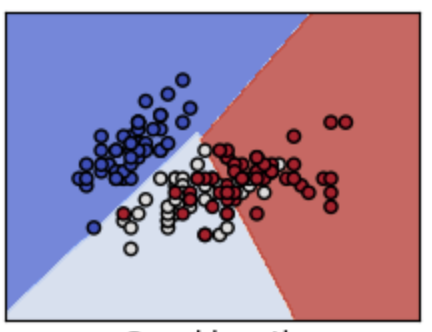
\includegraphics[scale=0.8]{imagenes/capitulo5/Entrenamiento/klineal.png}
	\caption{Kernel lineal}
	\label{fig:cp5:klineal}
	\end{subfigure}%
	\begin{subfigure}{.5\textwidth}
	\centering
	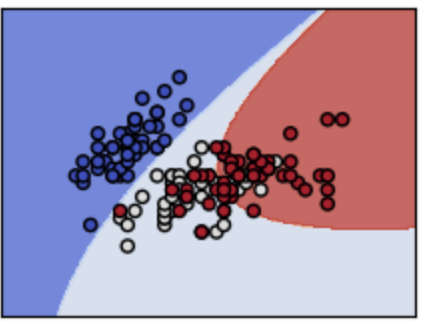
\includegraphics[scale=0.8]{imagenes/capitulo5/Entrenamiento/kpoli.png}
	\caption{Kernel polinomial}
	\label{fig:cp5:kpoli}
	\end{subfigure}%
\caption{Kernel de la función \citep{CC1}}
\end{figure}

\begin{figure}[H]
\centering
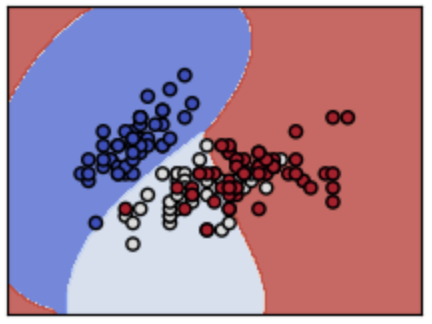
\includegraphics[scale=0.8]{imagenes/capitulo5/Entrenamiento/krbf.png}
\caption{Kernel radial \citep{CC1}}
\label{fig:cp5:krbf}
\end{figure}


Ahora se han explicado todos los parámetros de los algoritmos. Para las pruebas de este trabajo terminal han implementado 5 pliegues en la validación cruzada y se ha usado el corpus con 3150 noticias. Los resultados son visualizados en las siguientes tablas, donde la primera columna \textbf{Parámetros} contiene los parámetros variados de cada prueba, las columnas siguientes \textbf{P1}, \textbf{P2}, \textbf{P3}, \textbf{P4} y \textbf{P5} muestran el \textbf{exactitud} obtenido en cada pliegue, la columna \textbf{Promedio} muestra la suma de los \textbf{exactitud} obtenidos divido entre 5 (número de pliegues) y la última columna \textbf{Rank} muestra un número entero el cual indica el \textit{Ranking} de cada prueba, es decir la prueba con rank 1 es el mejor resultado, la prueba con rank 2 es el segundo mejor y así sucesivamente.\\

\begin{table}[H]
\centering
\resizebox{\columnwidth}{!}{%
	\begin{tabular}{|l|l|l|l|l|l|l|l|}
	%-----------------------Ecanbezado-----------------------------------%
		\hline
\multicolumn{1}{| >{\columncolor{myBlueChapter}}l|}{ \textcolor{myWhite}{\textbf{Parámetros}} }&
\multicolumn{1}{| >{\columncolor{myBlueChapter}}l|}{ \textcolor{myWhite}{\textbf{P 1}} }&
\multicolumn{1}{| >{\columncolor{myBlueChapter}}l|}{ \textcolor{myWhite}{\textbf{P 2}} }&
\multicolumn{1}{| >{\columncolor{myBlueChapter}}l|}{ \textcolor{myWhite}{\textbf{P 3}} }&
\multicolumn{1}{| >{\columncolor{myBlueChapter}}l|}{ \textcolor{myWhite}{\textbf{P 4}} }&
\multicolumn{1}{| >{\columncolor{myBlueChapter}}l|}{ \textcolor{myWhite}{\textbf{P 5}} }&
\multicolumn{1}{| >{\columncolor{myBlueChapter}}l|}{ \textcolor{myWhite}{\textbf{Promedio}} }&
\multicolumn{1}{| >{\columncolor{myBlueChapter}}l|}{ \textcolor{myWhite}{\textbf{Rank}} }
\\  \cline{1-8}
	%--------------

alpha: 0.5&0.8610&0.8576&0.8458&0.8487&0.8424&0.8511&1\\
\hline
alpha: 1&0.8531&0.8497&0.8426&0.8408&0.8360&0.8444&2\\
\hline
alpha: 1.5&0.8531&0.8434&0.8410&0.8392&0.8312&0.8416&3\\
\hline
alpha: 2&0.8531&0.8418&0.8410&0.8392&0.8296&0.8409&4\\
\hline

	\end{tabular}
}
\caption{Naive bayes}
\label{tab:cp5:naive}
\end{table}


\begin{table}[H]
\centering
\resizebox{\columnwidth}{!}{%
	\begin{tabular}{|l|l|l|l|l|l|l|l|}
	%-----------------------Ecanbezado-----------------------------------%
		\hline
\multicolumn{1}{| >{\columncolor{myBlueChapter}}l|}{ \textcolor{myWhite}{\textbf{Parámetros}} }&
\multicolumn{1}{| >{\columncolor{myBlueChapter}}l|}{ \textcolor{myWhite}{\textbf{P 1}} }&
\multicolumn{1}{| >{\columncolor{myBlueChapter}}l|}{ \textcolor{myWhite}{\textbf{P 2}} }&
\multicolumn{1}{| >{\columncolor{myBlueChapter}}l|}{ \textcolor{myWhite}{\textbf{P 3}} }&
\multicolumn{1}{| >{\columncolor{myBlueChapter}}l|}{ \textcolor{myWhite}{\textbf{P 4}} }&
\multicolumn{1}{| >{\columncolor{myBlueChapter}}l|}{ \textcolor{myWhite}{\textbf{P 5}} }&
\multicolumn{1}{| >{\columncolor{myBlueChapter}}l|}{ \textcolor{myWhite}{\textbf{Promedio}} }&
\multicolumn{1}{| >{\columncolor{myBlueChapter}}l|}{ \textcolor{myWhite}{\textbf{Rank}} }
\\  \cline{1-8}
	%--------------
C: 0.1, penalty: l2, solver: liblinear&0.8768&0.8655&0.8521&0.8710&0.8758&0.8682&1\\
\hline
C: 0.01, penalty: l2, solver: liblinear&0.8705&0.8655&0.8474&0.8742&0.8615&0.8638&2\\
\hline
C: 0.1, penalty: l1, solver: liblinear&0.8515&0.8544&0.8442&0.8424&0.8376&0.8460&3\\
\hline
C: 0.001, penalty: l2, solver: liblinear&0.8436&0.8560&0.8299&0.8392&0.8169&0.8371&4\\
\hline
C: 0.0001, penalty: l2, solver: liblinear&0.7836&0.7832&0.7806&0.7739&0.7723&0.7787&5\\
\hline
C: 0.01, penalty: l1, solver: liblinear&0.6477&0.6297&0.5946&0.6099&0.6099&0.6184&6\\
\hline
C: 1e-05, penalty: l2, solver: liblinear&0.6051&0.6044&0.6057&0.5924&0.5796&0.5974&7\\
\hline
C: 1e-06, penalty: l2, solver: liblinear&0.5261&0.5316&0.5564&0.5223&0.5048&0.5282&8\\
\hline
C: 1e-06, penalty: l1, solver: liblinear&0.2006&0.2009&0.2003&0.2006&0.2006&0.2006&9\\
\hline
C: 1e-05, penalty: l1, solver: liblinear&0.2006&0.2009&0.2003&0.2006&0.2006&0.2006&9\\
\hline
C: 0.0001, penalty: l1, solver: liblinear&0.2006&0.2009&0.2003&0.2006&0.2006&0.2006&9\\
\hline
C: 0.001, penalty: l1, solver: liblinear&0.2006&0.2009&0.2003&0.2006&0.2006&0.2006&9\\
\hline
	\end{tabular}
}
\caption{Regresión logística}
\label{tab:cp5:regresion}
\end{table}


\begin{table}[H]
\centering
\resizebox{\columnwidth}{!}{%
	\begin{tabular}{|l|l|l|l|l|l|l|l|}
	%-----------------------Ecanbezado-----------------------------------%
		\hline
\multicolumn{1}{| >{\columncolor{myBlueChapter}}l|}{ \textcolor{myWhite}{\textbf{Parámetros}} }&
\multicolumn{1}{| >{\columncolor{myBlueChapter}}l|}{ \textcolor{myWhite}{\textbf{P 1}} }&
\multicolumn{1}{| >{\columncolor{myBlueChapter}}l|}{ \textcolor{myWhite}{\textbf{P 2}} }&
\multicolumn{1}{| >{\columncolor{myBlueChapter}}l|}{ \textcolor{myWhite}{\textbf{P 3}} }&
\multicolumn{1}{| >{\columncolor{myBlueChapter}}l|}{ \textcolor{myWhite}{\textbf{P 4}} }&
\multicolumn{1}{| >{\columncolor{myBlueChapter}}l|}{ \textcolor{myWhite}{\textbf{P 5}} }&
\multicolumn{1}{| >{\columncolor{myBlueChapter}}l|}{ \textcolor{myWhite}{\textbf{Promedio}} }&
\multicolumn{1}{| >{\columncolor{myBlueChapter}}l|}{ \textcolor{myWhite}{\textbf{Rank}} }
\\  \cline{1-8}
	%--------------
max\_depth: 50, n\_estimators: 1000&0.8720&0.8592&0.8537&0.8631&0.8615&0.8619&1\\
\hline
max\_depth: 1000, n\_estimators: 1000&0.8689&0.8639&0.8585&0.8583&0.8583&0.8616&2\\
\hline
max\_depth: 100, n\_estimators: 1000&0.8752&0.8592&0.8569&0.8599&0.8551&0.8613&3\\
\hline
max\_depth: 100, n\_estimators: 500&0.8784&0.8608&0.8601&0.8535&0.8519&0.8609&4\\
\hline
max\_depth: 1000, n\_estimators: 500&0.8720&0.8528&0.8585&0.8551&0.8599&0.8597&5\\
\hline
max\_depth: 50, n\_estimators: 500&0.8705&0.8544&0.8601&0.8535&0.8599&0.8597&6\\
\hline
max\_depth: 500, n\_estimators: 1000&0.8720&0.8655&0.8506&0.8487&0.8583&0.8590&7\\
\hline
max\_depth: 500, n\_estimators: 500&0.8689&0.8544&0.8553&0.8519&0.8615&0.8584&8\\
\hline
max\_depth: 500, n\_estimators: 100&0.8610&0.8608&0.8506&0.8487&0.8662&0.8575&9\\
\hline
max\_depth: 50, n\_estimators: 100&0.8641&0.8528&0.8601&0.8503&0.8455&0.8546&10\\
\hline
max\_depth: 1000, n\_estimators: 100&0.8594&0.8528&0.8474&0.8392&0.8439&0.8485&11\\
\hline
max\_depth: 100, n\_estimators: 100&0.8657&0.8560&0.8394&0.8471&0.8280&0.8473&12\\
\hline
max\_depth: 50, n\_estimators: 50&0.8626&0.8402&0.8267&0.8583&0.8471&0.8470&13\\
\hline
max\_depth: 100, n\_estimators: 50&0.8420&0.8402&0.8283&0.8503&0.8535&0.8429&14\\
\hline
max\_depth: 500, n\_estimators: 50&0.8531&0.8418&0.8331&0.8424&0.8312&0.8403&15\\
\hline
max\_depth: 1000, n\_estimators: 50&0.8578&0.8212&0.8315&0.8392&0.8280&0.8355&16\\
\hline
	\end{tabular}
}
\caption{Random Forest}
\label{tab:cp5:random}
\end{table}


\begin{table}[H]
\centering
\resizebox{\columnwidth}{!}{%
	\begin{tabular}{|l|l|l|l|l|l|l|l|}
	%-----------------------Ecanbezado-----------------------------------%
		\hline
\multicolumn{1}{| >{\columncolor{myBlueChapter}}l|}{ \textcolor{myWhite}{\textbf{Parámetros}} }&
\multicolumn{1}{| >{\columncolor{myBlueChapter}}l|}{ \textcolor{myWhite}{\textbf{P 1}} }&
\multicolumn{1}{| >{\columncolor{myBlueChapter}}l|}{ \textcolor{myWhite}{\textbf{P 2}} }&
\multicolumn{1}{| >{\columncolor{myBlueChapter}}l|}{ \textcolor{myWhite}{\textbf{P 3}} }&
\multicolumn{1}{| >{\columncolor{myBlueChapter}}l|}{ \textcolor{myWhite}{\textbf{P 4}} }&
\multicolumn{1}{| >{\columncolor{myBlueChapter}}l|}{ \textcolor{myWhite}{\textbf{P 5}} }&
\multicolumn{1}{| >{\columncolor{myBlueChapter}}l|}{ \textcolor{myWhite}{\textbf{Promedio}} }&
\multicolumn{1}{| >{\columncolor{myBlueChapter}}l|}{ \textcolor{myWhite}{\textbf{Rank}} }
\\  \cline{1-8}
	%------------------------------------------------%
C: 100, gamma: 0.0001, kernel: rbf&0.8736&0.8639&0.8537&0.8726&0.8822&0.8692&1\\
\hline
C: 1000, gamma: 1e-05, kernel: rbf&0.8752&0.8623&0.8537&0.8710&0.8822&0.8689&2\\
\hline
C: 1000, gamma: 0.0001, kernel: rbf&0.8689&0.8608&0.8506&0.8694&0.8790&0.8657&3\\
\hline
C: 1, gamma: 0.0001, kernel: linear&0.8657&0.8592&0.8410&0.8710&0.8742&0.8622&4\\
\hline
C: 1, gamma: 1e-05, kernel: linear&0.8657&0.8592&0.8410&0.8710&0.8742&0.8622&4\\
\hline
C: 1, gamma: 1e-06, kernel: linear&0.8657&0.8592&0.8410&0.8710&0.8742&0.8622&4\\
\hline
C: 10, gamma: 0.0001, kernel: linear&0.8657&0.8592&0.8394&0.8710&0.8742&0.8619&5\\
\hline
C: 10, gamma: 1e-05, kernel: linear&0.8657&0.8592&0.8394&0.8710&0.8742&0.8619&5\\
\hline
C: 10, gamma: 1e-06, kernel: linear&0.8657&0.8592&0.8394&0.8710&0.8742&0.8619&5\\
\hline
C: 100, gamma: 0.0001, kernel: linear&0.8657&0.8592&0.8394&0.8710&0.8742&0.8619&5\\
\hline
C: 100, gamma: 1e-05, kernel: linear&0.8657&0.8592&0.8394&0.8710&0.8742&0.8619&5\\
\hline
C: 100, gamma: 1e-06, kernel: linear&0.8657&0.8592&0.8394&0.8710&0.8742&0.8619&5\\
\hline
C: 1000, gamma: 0.0001, kernel: linear&0.8657&0.8592&0.8394&0.8710&0.8742&0.8619&5\\
\hline
C: 1000, gamma: 1e-05, kernel: linear&0.8657&0.8592&0.8394&0.8710&0.8742&0.8619&5\\
\hline
C: 1000, gamma: 1e-06, kernel: linear&0.8657&0.8592&0.8394&0.8710&0.8742&0.8619&5\\
\hline
C: 10, gamma: 0.0001, kernel: rbf&0.8641&0.8576&0.8490&0.8678&0.8503&0.8578&6\\
\hline
C: 100, gamma: 1e-05, kernel: rbf&0.8641&0.8576&0.8490&0.8662&0.8519&0.8578&6\\
\hline
C: 1000, gamma: 1e-06, kernel: rbf&0.8641&0.8576&0.8490&0.8662&0.8519&0.8578&6\\
\hline
C: 100, gamma: 1e-06, kernel: rbf&0.6524&0.6772&0.6073&0.6449&0.6608&0.6485&7\\
\hline
C: 10, gamma: 1e-05, kernel: rbf&0.6493&0.6741&0.6073&0.6401&0.6561&0.6454&8\\
\hline
C: 1, gamma: 0.0001, kernel: rbf&0.6193&0.6440&0.5946&0.6115&0.6306&0.6200&9\\
\hline
C: 1, gamma: 0.0001, kernel: poly&0.2038&0.2041&0.2035&0.2038&0.2038&0.2038&10\\
\hline
C: 1, gamma: 1e-05, kernel: poly&0.2038&0.2041&0.2035&0.2038&0.2038&0.2038&10\\
\hline
C: 1, gamma: 1e-05, kernel: rbf&0.2038&0.2041&0.2035&0.2038&0.2038&0.2038&10\\
\hline
C: 1, gamma: 1e-06, kernel: poly&0.2038&0.2041&0.2035&0.2038&0.2038&0.2038&10\\
\hline
C: 1, gamma: 1e-06, kernel: rbf&0.2038&0.2041&0.2035&0.2038&0.2038&0.2038&10\\
\hline
C: 10, gamma: 0.0001, kernel: poly&0.2038&0.2041&0.2035&0.2038&0.2038&0.2038&10\\
\hline
C: 10, gamma: 1e-05, kernel: poly&0.2038&0.2041&0.2035&0.2038&0.2038&0.2038&10\\
\hline
C: 10, gamma: 1e-06, kernel: poly&0.2038&0.2041&0.2035&0.2038&0.2038&0.2038&10\\
\hline
C: 10, gamma: 1e-06, kernel: rbf&0.2038&0.2041&0.2035&0.2038&0.2038&0.2038&10\\
\hline
C: 100, gamma: 0.0001, kernel: poly&0.2038&0.2041&0.2035&0.2038&0.2038&0.2038&10\\
\hline
C: 100, gamma: 1e-05, kernel: poly&0.2038&0.2041&0.2035&0.2038&0.2038&0.2038&10\\
\hline
C: 100, gamma: 1e-06, kernel: poly&0.2038&0.2041&0.2035&0.2038&0.2038&0.2038&10\\
\hline
C: 1000, gamma: 0.0001, kernel: poly&0.2038&0.2041&0.2035&0.2038&0.2038&0.2038&10\\
\hline
C: 1000, gamma: 1e-05, kernel: poly&0.2038&0.2041&0.2035&0.2038&0.2038&0.2038&10\\
\hline
C: 1000, gamma: 1e-06, kernel: poly&0.2038&0.2041&0.2035&0.2038&0.2038&0.2038&10\\
\hline

	\end{tabular}
}
\caption{Máquina de soporte vectorial}
\label{tab:cp5:msv}
\end{table}




%------------------------------------------------------------------%
\subsection{Selección}


Los resultados de la sección anterior ha mostrado que no existe una brecha muy grande en el \textbf{exactitud} obtenido de los mejores parámetros, como se muestra en la siguiente Tabla (\ref{tab:cp5:resultados}).

\begin{table}[H]
\centering
	\begin{tabular}{|l|c|c|}
	%-----------------------Ecanbezado-----------------------------------%
		\hline
\multicolumn{1}{| >{\columncolor{myBlueChapter}}l|}{ \textcolor{myWhite}{\textbf{Algoritmo}} }&
\multicolumn{1}{| >{\columncolor{myBlueChapter}}l|}{ \textcolor{myWhite}{\textbf{Exactitud}} }&
\multicolumn{1}{| >{\columncolor{myBlueChapter}}l|}{ \textcolor{myWhite}{\textbf{Ranking}} }
\\  \cline{1-3}
	%--------------

MSV&0.8692&1\\
\hline
Regresión Logística&0.8682&2\\
\hline
Random Forest&0.8619&3\\
\hline
Naive Bayes&0.8511&4\\
\hline
	\end{tabular}
\caption{Precisión de los mejores parámetros}
\label{tab:cp5:resultados}
\end{table}


El mejor resultado se ha conseguido con el algoritmo \textbf{Máquina de soporte vectorial} con los parámetros ;$C$=100, $gamma$=0.0001 y $kernel$= $rbf$ (radial) obteniendo 0.8619 de \textbf{exactitud}, por esta razón se ha elegido como el clasificador final de este trabajo terminal.

%------------------------------------------------------------------%
\subsection{Pruebas}

Con base en el algoritmo elegido y los parámetros que han conseguido obtener el mejor resultado, se ha hecho una prueba final, la cual consiste en clasificar el corpus de prueba con 350 noticias, creado al final de la sección de pre-procesamiento (ver \Tref{cp5:divisionC}{División del corpus}  ), para calcular la matriz de confusión y obtener las métricas de evaluación. La tabla \ref{tab:cp5:numnoticias} muestra el número de noticias por sección contenidas en el corpus.\\

\begin{table}[H]
\centering
	\begin{tabular}{|l|c|}
	%-----------------------Ecanbezado-----------------------------------%
		\hline
\multicolumn{1}{| >{\columncolor{myBlueChapter}}l|}{ \textcolor{myWhite}{\textbf{Sección}} }&
\multicolumn{1}{| >{\columncolor{myBlueChapter}}l|}{ \textcolor{myWhite}{\textbf{Número de noticias}} }
\\  \cline{1-2}
	%--------------

Deportes& 68\\
\hline
Economía& 58\\
\hline
Política& 69\\
\hline
Cultura& 77\\
\hline
Ciencia y Tecnología& 78\\
\hline
	\end{tabular}
\caption{Número de noticias}
\label{tab:cp5:numnoticias}
\end{table}


La matriz de confusión obtenida se muestra en la tabla \ref{tab:cp5:matriz}, donde las filas representan la clasificación real de la noticia y las columnas lo predicho por el clasificador. Por ejemplo se observa que en la sección \textbf{Deportes} de 68 noticias etiquetadas, 65 fueron clasificadas correctamente, y 3 fueron mal clasificadas en la sección \textbf{ciencia y tecnología} (1 noticia), \textbf{economía} (1 noticia) y \textbf{política} (1 noticia). En la sección de ciencia y tecnología de 78 noticias solo 67 fueron clasificadas de forma acertada, y 11 fueron clasificadas en las distintas secciones: 1 en \textbf{Deportes}, 5 en \textbf{Economía}, 3 en \textbf{Política} y 2 en \textbf{Cultura}.\\

\begin{table}[H]
\centering
\resizebox{\columnwidth}{!}{%
	\begin{tabular}{|l|c|c|c|c|c|}
	%-----------------------Ecanbezado-----------------------------------%
		\hline
\multicolumn{1}{| >{\columncolor{myBlueChapter}}l|}{ \textcolor{myWhite}{\textbf{Sección}} }&
\multicolumn{1}{| >{\columncolor{myBlueChapter}}l|}{ \textcolor{myWhite}{\textbf{Deportes}} }&
\multicolumn{1}{| >{\columncolor{myBlueChapter}}l|}{ \textcolor{myWhite}{\textbf{Economía}} }&
\multicolumn{1}{| >{\columncolor{myBlueChapter}}l|}{ \textcolor{myWhite}{\textbf{Política}} }&
\multicolumn{1}{| >{\columncolor{myBlueChapter}}l|}{ \textcolor{myWhite}{\textbf{Cultura}} }&
\multicolumn{1}{| >{\columncolor{myBlueChapter}}l|}{ \textcolor{myWhite}{\textbf{Cienci y T}} }
\\  \cline{1-6}
	%--------------

Deportes& 65 & 1 & 1 & 0 & 1\\
\hline
Economía& 1 & 51 & 4 & 1 & 1\\
\hline
Política& 2 & 5 & 59 & 3 & 0\\
\hline
Cultura& 1 & 1 & 1 & 70 & 4\\
\hline
Ciencia y T& 1 & 5 & 3 & 2 & 67\\
\hline
	\end{tabular}
}
\caption{Matriz de confusión}
\label{tab:cp5:matriz}
\end{table}


Con base en la matriz de confusión se ha calculado \textbf{Recall}, \textbf{Fmeasure}, \textbf{Precision} (ver \Tref{cp3:metricase}{Métricas de evaluación}). Las métricas son obtenidas por cada sección, como se muestra en la tabla \ref{tab:cp5:metricas}.

\begin{table}[H]
\centering
	\begin{tabular}{|l|c|c|c|}
	%-----------------------Ecanbezado-----------------------------------%
		\hline
\multicolumn{1}{| >{\columncolor{myBlueChapter}}l|}{ \textcolor{myWhite}{\textbf{Sección}} }&
\multicolumn{1}{| >{\columncolor{myBlueChapter}}l|}{ \textcolor{myWhite}{\textbf{Precision}} }&
\multicolumn{1}{| >{\columncolor{myBlueChapter}}l|}{ \textcolor{myWhite}{\textbf{Recall}} }&
\multicolumn{1}{| >{\columncolor{myBlueChapter}}l|}{ \textcolor{myWhite}{\textbf{F-measuere}} }
\\  \cline{1-4}
	%--------------

Deportes & 0.93 & 0.96 & 0.94\\
\hline
Economía & 0.81 & 0.88 & 0.84\\
\hline
Política & 0.87 & 0.86 & 0.86\\
\hline
Cultura & 0.92 & 0.91 & 0.92\\
\hline
Ciencia y Tecnología & 0.92 & 0.86 & 0.89\\
\hline
	\end{tabular}
\caption{Metricas de evaluación}
\label{tab:cp5:metricas}
\end{table}


Como se puede observar en la tabla \ref{tab:cp5:metricas} las sección con mejor \textbf{Fmeasure} (este valor sostiene una relación entre \textbf{Precision} y \textbf{Recall}) es \textbf{Deportes} obteniendo 0.94 en la clasificación. Este resultado se puede explicar con base en el vocabulario manejado en la categoría, ya que es muy específico, por ejemplo se usan palabras como: gol, jugador, resultado, anotación. Por lo contrario el \textbf{Fmeasure} mas bajo lo obtuvo \textbf{Economía} con 0.84 (el cual no es un mal resultado), las palabras manejadas por esta sección pueden ser encontradas en otras categorías, generando así confusión en la clasificación.\\

Finalmente, considerando la exactitud de de todas las secciones, el modelo entrenado obtuvo una exactitud promedio de 0.89. Este resultado es muy bueno considerando que los trabajos descritos en el estado del arte (ver \Tref{cp2:estadodelarte}{Estado del arte}) obtienen una exactitud entre 0.80 y 0.90




%------------------------------------------------------------------%
\Tlabel{cp5:persistencia}
\subsection{Persistencia}


Como última etapa de la clasificación, el modelo \textbf{Máquina de soporte vectorial} debe ser almacenado así como las características del corpus. Para esta tarea se ha utilizado el corpus completo de 3500 noticias, del cual se extraen las características, se entrena el modelo y estos conjuntos son almacenados en un archivo ocupando la biblioteca \textbf{pickle}, de esta forma en la siguiente sección el modelo es utilizado como parte de la \textbf{Aplicación web}.



%\subsection{Tokenizar}
%\subsection{Lematizar}
%\subsection{Validación cruzada}
%\subsection{Shuffle}
%\subsection{Grid search}
%\subsection[Resultados]{Selección y resultado del mejor clasificador}
%\subsection[Persistencia]{Persistencia del clasificador}
\newpage
\section{Aplicación web}

La siguiente Figura \ref{fig:procesoApp} muestra las etapas que se llevarán a cabo por parte de la aplicación web.
\begin{figure}[ht]
\centering
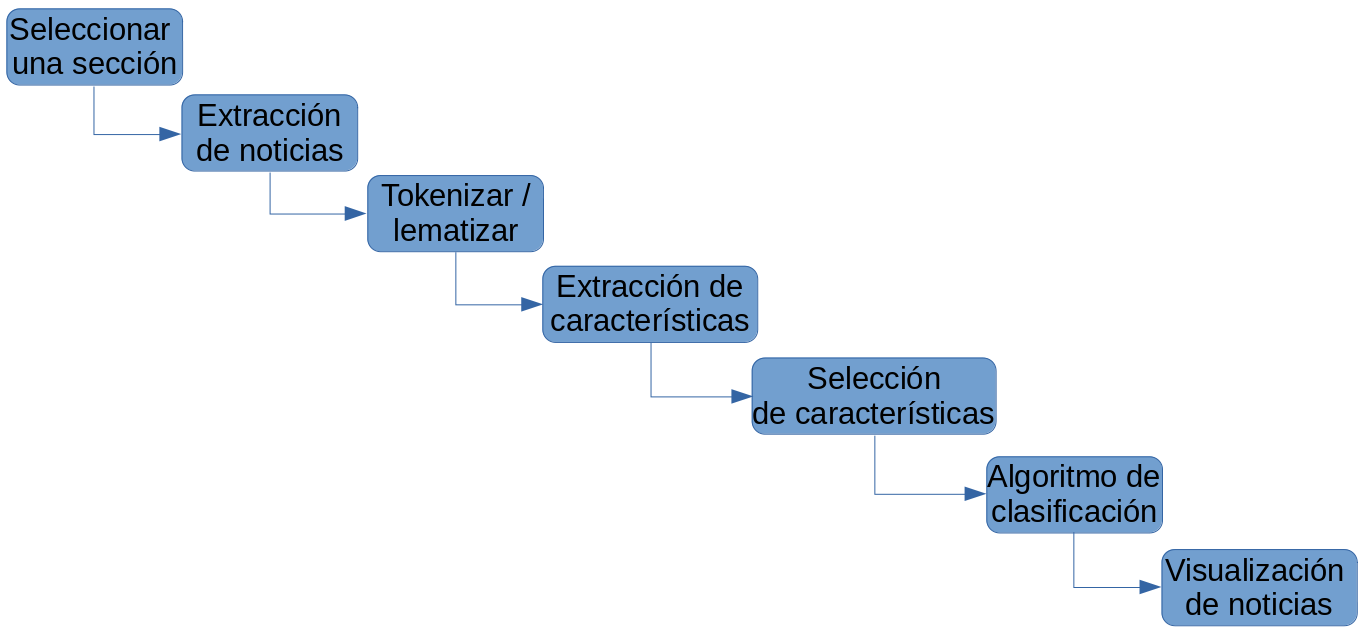
\includegraphics[scale=0.3]{imagenes/Capitulo5/procesoAplicacionWeb.png}
\caption{Etapas de la aplicación web}
\label{fig:procesoApp}
\end{figure}

\subsection{Proceso de recolección}
La aplicación web tiene como objetivo recolectar y clasificar noticias, por ello la primera parte que se debe realizar es la recolección de noticias, como se mencionó en el apartado 5.1 se han definido los sitios web de donde las noticias serán recolectadas, la información recuperada śerá:

\begin{itemize}
	\item URL de la noticia
	\item Título
	\item Fecha
	\item Autor
	\item Descripción \footnote{Existen sitios web, donde no todas las noticias cuentan con una descripción}
	\item Noticia
\end{itemize}

Cabe destacar que en este punto, ya no será necesario extraer el nombre de la sección a la cual pertenece la noticia.
\\
\subsection{Proceso de clasificación}
Una vez que las noticias han sido recolectadas, deberán pasar por dos pasos fundamentales, como primer paso la noticia debe ser tokenizada y lematizada, posteriormente se deben extraer las características de cada noticia, esto permitirá al algoritmo seleccionado tener una mejor precisión en el momento de realizar la clasificación, 
para finalizar las noticias serán clasificadas.

\subsection{Frontend}

Para la realización de la aplicación web es necesario utilizar herramientas que nos permitan visualizar las noticias clasificadas, por ello las interfaces de usuario se desarrollarón en utilizando el Framework Java Server Faces.

La Figura \ref{fig:PantallaInicio} muestra la vista que tendrá el usuario al ingresar a la aplicación web

\begin{figure}[ht]
\centering
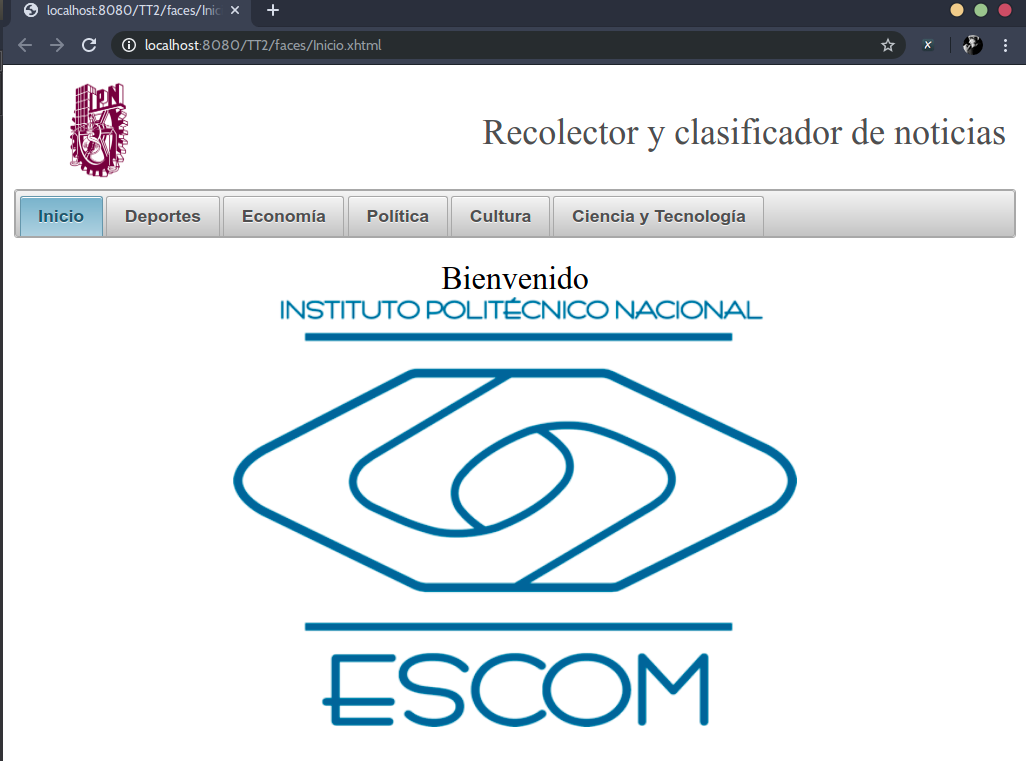
\includegraphics[scale=0.3]{imagenes/Capitulo5/inicio.png}
\caption{Pantalla de Inicio.}
\label{fig:PantallaInicio}
\end{figure}

El usuario tiene la posibilidad de elegir la sección de la cual desee visualizar noticias. La Figura \ref{fig:loading} muestra la vista que tendrá el usuario dar click en una sección.

\begin{figure}[ht]
\centering
\includegraphics[scale=0.3]{imagenes/Capitulo5/cargando.png}
\caption{Pantalla de espera}
\label{fig:loading}
\end{figure}

Una vez finalizado el proceso de recolección de noticias


El proceso que se llevará a cabo para poder visualizar 
Para visualizar
	Aplicación web
		Archivo físico
		ya no se busca por sección 
		hacer menció de casos de uso






  
  %-------------------------------Bibliografía----------%
  \bibliography{Capitulos/Referencia}


\end{document}
